%!TEX TS-program = xelatex
%!TEX encoding = UTF-8 Unicode
\documentclass[School=Harvard]{Dissertate}


\usepackage{algpseudocode}
\usepackage{algorithm2e}
\usepackage{float}
\usepackage{subcaption}
\usepackage{graphicx}
\usepackage{wrapfig}
\usepackage{minted}
\usepackage{xurl}
\usepackage{microtype}
\usepackage{rotating}
\usepackage{enumitem}
\raggedbottom
\usepackage[export]{adjustbox}
\usepackage[column=0]{cellspace}
\setlength{\cellspacetoplimit}{\tabcolsep}
\setlength{\cellspacebottomlimit}{\tabcolsep}

% \usepackage[footnote]{acronym}
\usepackage[symbol]{footmisc}

\usepackage{perpage}
\MakePerPage{footnote}
\renewcommand{\thefootnote}{\fnsymbol{footnote}}

\begin{document}

% the front matter
% Some details about the dissertation.
\title{Title of the dissertation}
\author{Maciej W. Majewski}
\advisor{dr hab. inż. Tomasz Szumlak}

% ... about the degree.
% \degree{Doctor of Philosophy}
% \field{Psychology}
% \degreeyear{2024}
% \degreemonth{May}
% \department{Psychology}

% % ... about the candidate's previous degrees.
% \pdOneName{B.S.}
% \pdOneSchool{Boston University}
% \pdOneYear{2018}

% \pdTwoName{M.A.}
% \pdTwoSchool{Monster's Univeristy}
% \pdTwoYear{2021}

\setmintedinline{fontsize=\footnotesize}

\maketitle
% \copyrightpage
\abstractpage
%\listoffigures
% \dedicationpage
\acknowledgments
% \authorcontribution
\tableofcontents


\onehalfspacing

% include each chapter...
\setcounter{chapter}{-1}  % start chapter numbering at 0
\begin{savequote}[75mm]
In the beginning there was nothing, which exploded.
\qauthor{Terry Pratchett}
\end{savequote}

\chapter{Introduction}
\label{introduction}

In a brief moment, a universe happened.
After the Big Bang, the matter (leptons and quarks that form protons and neutrons) came to life following a brief period known as inflation.
The currently known physics says that an equal amount of antimatter (to compliment the matter) should be produced as well.
Yet, we do not observe the universe to be symmetrical, cosmic yin-yang; equal parts matter and antimatter.
This is one of the greatest riddles of current physics.
One of the goals of the LHCb experiment at CERN is to find and study the processes that can contribute to this asymmetry.

The grand promise of the modern physics is the theory of everything; a universe boiled down to a single theory, perhaps even to a single equation.
This dream is partially realised by the Standard Model, the theory that describes three fundamental forces (interactions) in physics.
Weak nuclear, strong nuclear, and electromagnetic force, come together into a single equation.
To some, it may be surprising that all of the mechanics in the known universe can be rooted just in a single theory based on the principle of local gauge invariance.
But the emergence of complex mechanisms from simple rules is prevalent in science.
Game of Life - a cellular automata simulation, although containing a small set of rules can make increasingly complex structures.
Most of the known chemistry that guides the biological processes, can be explained almost exclusively "just" using the electrical potential and probability.

As particle physicists, we see this emergence of complexity even at a very basic level.
By colliding two protons, we see a multitude of emergent possibilities, many different particles, and a vast sea of probable combinations of fundamental building blocks.
Studying those combinations of possibilities is the bread and butter of modern particle physics.
One of the misconceptions about High Energy Physics is that it is like a grandiose hunt through a murky and empty Forrest for one big prey.

In reality, it is more like being an explorer of new land.
Every day we check new jungle parts, expecting to find the trees and maybe some new species of the forest flora, and we see precisely that.
On some days, we revisit some parts to see if we notice anything extraordinary.
But still, we hope that we will find an ancient city of unknown civilisation with unimaginable treasure that will change everything that we know.
And we can't deny it does not exist until we search through all of the continent.
For particle physicists, this treasure is physics beyond the Standard Model.

This steady, monotone and patient work of checking all of the branches of physics is facilitated by the international community of scientists, of which CERN scientists constitute by far the largest group, with the biggest particle accelerator - LHC (Large Hadron Collider).
The LHC is a circular accelerator located in the underground tunnel under the Swiss-French border.
A large portion of the physicist working at CERN are parts of four main experiments Alice, Atlas, CMS and LHCb.
During my PhD studies, I was privileged to be one of the collaborators in the LHCb experiment.
The LHCb experiment discovered so far 54 new particles while analysing the collected data samples.
Such extraordinary science done with the LHCb spectrometer couldn't be possible without years of preparation and without overcoming technical challenges posed by the physics and the hardware.
Cooling systems, electronics, mechanic design, software, tracking, particle identification, all of the subsystems, and parts of the detector spawn new problems to be solved by the collaboration and the greater scientific community.
I am glad to introduce the reader to my thesis, describing some solutions to those problems.

\begin{savequote}[75mm]
  There is no unique picture of reality.
  \qauthor{Stephen Hawking}
\end{savequote}

\chapter{High Energy Physics}

The idea of atoms - building blocks of nature stretches back as far as ancient Greece, to Leucippus and Democritus \cite{10.3138/9781442671102}, and prevailed through the ages until the beginning of the 20th century, when it was solidified. In 1897 J.J.Thompson discovered an electron using a cathode ray and noticed its negative charge \cite{thomson1901bodies}.
Later in 1911, Rutherford discovered the nucleus using the gold foil scattering experiment \cite{doi:10.1080/14786440508637080}.
Shortly after that, in 1932, the model of the nucleus containing neutron and proton was developed \cite{Iwanenko1932TheNH, 1932ZPhy...77....1H}.
These events, along with the development of quantum mechanics, laid a foundation for the development of modern physics.
The deeper we wanted to look inside the matter, and the deeper it  was probed by the physics, the more different particles were found.
This ``particle zoo'' was later explained with Quantum Field Theory and a small number of fundamental particles.
Those fundamental particles and the rules that guide their interactions are combined into Standard Model - the best theory developed by our civilisation so far.

\section{Standard Model}

\begin{figure}
  \centering
  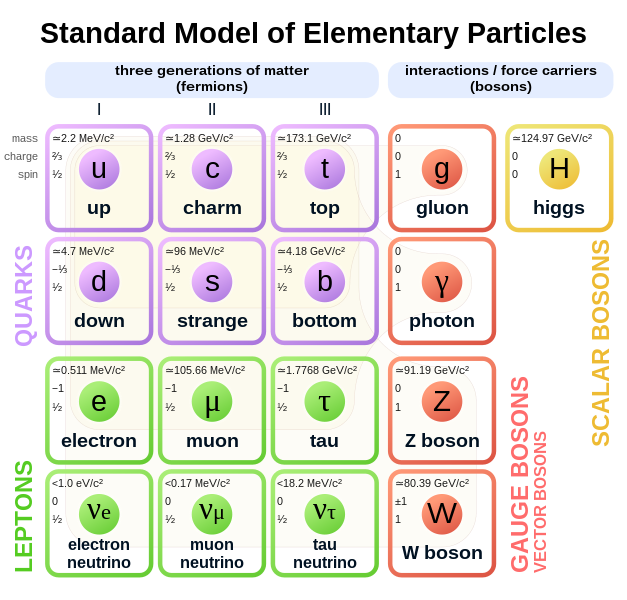
\includegraphics[width=0.7\linewidth]{figures/chapter1/Standard_Model_of_Elementary_Particles.svg.png}
  \caption[caption for LOF]{Standard model of Elementary Particles \footnotemark}
  \label{fig:standard_model}
\end{figure}
\footnotetext{ Source \url{https://en.wikipedia.org/wiki/File:Standard_Model_of_Elementary_Particles.svg}}


Standard model (schematically depicted in Fig. \ref{fig:standard_model}) consists of two types of particles: bosons and fermions. Bosons are responsible for the interactions, and fermions constitute matter (Neutrons, Protons, Atoms).
Furtherly, the fermions consist of three generations of leptons and quarks.
There are six quarks: up, down, charm, strange, top, and beauty. Two up quarks and one down quark combine into a proton, and one up quark and two down quarks combine into a neutron.
The combinations of quarks create the particle zoo. In fact, the quarks have never been observed as free particles, which is explained by the colour confinement.
The most popular combinations of quarks consist of two (mesons - quark and antiquark pair) and three quarks, with other combinations like pentaquarks much less probable but still possible.
Half of the fermions are leptons and have been observed as free particles, unlike quarks. The three charged leptons are electron, muon, and tau; all have an electric charge of -1.
The other three are three flavours of neutrinos: electron neutrino, muon neutrino, tau neutrino.
The neutrinos are charge-less and have a negligibly small mass. Due to that, they are very elusive and hard to study.

The Bosons are the particles that carry the interactions. There are twelve gauge vector bosons and one scalar boson.
The gauge bosons consist of a photon, eight gluons, two charged W bosons and one neutral Z boson.
The photon is a carrier of electromagnetic force and is massless and chargeless.
The strong nuclear force is propagated by gluons, which, similarly to the photon, are mass and charge-less, but unlike a photon, they can't exist as a free particle and carry the colour charge.
The W and Z bosons are responsible for the weak nuclear force.
Their exchange can change the flavour of the interacting quark or lepton.
The one scalar boson - the Higgs boson, is famously the newest addition to Standard Model.
The Higgs boson is responsible for attributing mass to W and Z bosons and fermions.

Additionally to the particles described above, each fermion has a corresponding anti-matter partner. In case of bosons we assume, according to Standard Model, that they are their own antiparicles (apart from W bosons).

The Large Hadron Collider and its accompanying detectors were created to study various implications of Standard Model. A few of the LHCb experiment's primary goals are presented below.


% \section{proton proton collisions}
\section{CP symmetry violation}
One of the cosmology's greatest mysteries is the severe inequality between matter and anti-matter in the observable universe. The simple assumption would be that there should be equal amounts of matter and anti-matter if the rules of physics are the same for matter and anti-matter.
The most probable cause for such a state is that soon after the Big Bang, the C-, P- and CP-symmetries (\textbf{C} for the charge parity operation, \textbf{P} for the space parity operation) were broken what led to creation of significantly more matter than antimatter.
The CP violation study is conducted to explain this phenomenon.

The parity inversion operator, \textbf{P}, can be defined as a mirror inversion:

$$
P\psi(r) = \psi(-r)
$$

There used to be a belief that physics is invariant under this operation, which was verified in strong and electromagnetic interactions but was not verified in weak interactions \cite{PhysRev.104.254}.
This led to experiments showing that some of the reactions in beta decay do not occur as frequently as their mirror image.
The next idea was that although parity itself may not be conserved, the conjugation of the charge parity operator combined with the spatial parity one constitute an exact symmetry.
The charge parity operator can be defined as an operator which changes a particle into its anti-particle by changing the sign of its additive quantum numbers (e.g., the charge):
$$
C \, |\psi\rangle = | \bar{\psi}\rangle.
$$

The combined $CP$ symmetry is also broken \cite{PhysRevLett.13.138} in weak interactions. The LHCb reported a $CP$ violation in B meson \cite{PhysRevLett.110.221601} and charm decays \cite{PhysRevLett.122.211803}. The beauty decays can have the CP-asymmetry at the level of 80\%.

In the search for the invariant law of symmetry, an additional combination of $CPT$ symmetry ($T$ is the time-reversal operator) was proposed, which seems to be conserved in all known processes in Standard Model.

Although the studies have shown that there exist symmetry breaking processes in weak interactions of the quark sector, they do not explain the imbalance in matter and anti-matter in the universe.
An additional search for symmetry breaking in the lepton sector is also undergoing.


\section{Tree-level determination of the unitarity triangle angle γ - CKM matrix}

One of the most interesting hints of physics beyond the standard model comes from the weak force and its calculation of the CKM matrix values. The CKM (Cabibo-Kobayashi-Maskawa) matrix elements describe the strength of the flavour change in weak interactions. I.e. $V_{ud}$ is the probability of the down quark transforming into an up quark.
$$
\begin{bmatrix}  d'  \\  s'  \\  b'  \end{bmatrix} = \begin{bmatrix} V_\mathrm{ud} & V_\mathrm{us} & V_\mathrm{ub} \\ V_\mathrm{cd} & V_\mathrm{cs} & V_\mathrm{cb} \\ V_\mathrm{td} & V_\mathrm{ts} & V_\mathrm{tb} \end{bmatrix} \begin{bmatrix}  d  \\  s  \\  b  \end{bmatrix}
$$

The most recent approximation of the CKM matrix values \cite{10.1093/ptep/ptaa104}, is as follows:

$$
\begin{bmatrix}
|V_{ud}| & |V_{us}| & |V_{ub}| \\
|V_{cd}| & |V_{cs}| & |V_{cb}| \\
|V_{td}| & |V_{ts}| & |V_{tb}|
\end{bmatrix} = \begin{bmatrix}
0.97370 \pm 0.00014 & 0.2245 \pm 0.0008 & 0.00382 \pm 0.00024 \\
0.221 \pm 0.004 & 0.987 \pm 0.011 & 0.0410 \pm 0.0014 \\
0.0080 \pm 0.0003 & 0.0388 \pm 0.0011  & 1.013 \pm 0.030
\end{bmatrix}.
$$


The CKM matrix can be understood as a rotation matrix in 3D (SU(3)) and, therefore,e can be parametrised by independent angles.
It is helpful to use it with Wolfenstein parametrisation \cite{PhysRevLett.51.1945}, which allows parametrising the matrix in four independent values $\lambda$, $A$, $\rho$ , and $\nu$.

Such parametrisation allows for representation of the unitarity condition of the CKM $V_{ud}V*_{ub} + V_{cd}V*_{cb}+ * V_{td}V*_{tb} = 0$ as a triangle:


\begin{figure}
  \centering
  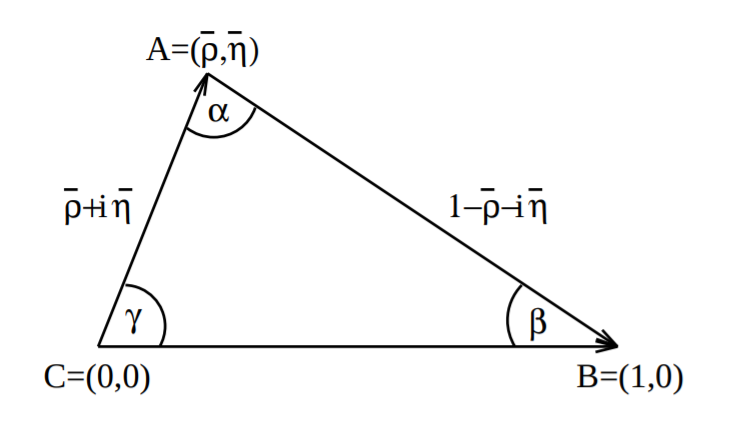
\includegraphics[width=0.6\linewidth]{figures/chapter1/UnitaryTriangle.png}
  \caption{A unitary triangle (source: \cite{buras2002unitarity})}
  \label{fig:unitary_triangle}
\end{figure}

Studies of various processes, mainly tree-level and loop processes, allow for calculating the constraints on the value of the $\gamma$ angle in the unitary triangle.


\begin{figure}[H]
\centering
\begin{subfigure}[b]{0.45\textwidth}
    \centering
    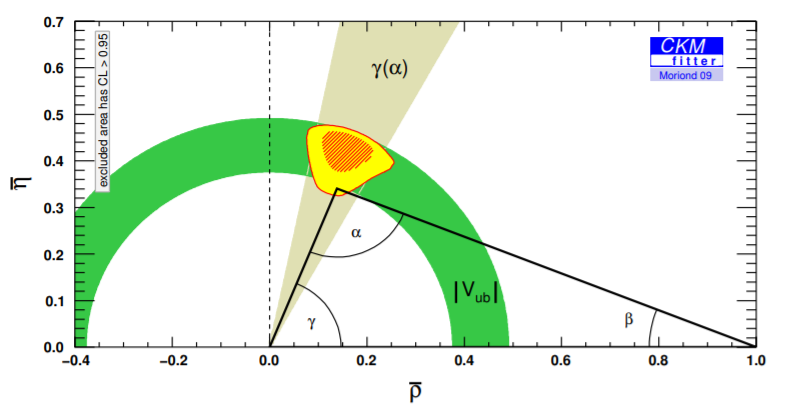
\includegraphics[width=\linewidth]{figures/chapter1/lhcb_goals_a.png}
\caption{}
   \label{plot:plot_triangle_a}
  \end{subfigure}
\begin{subfigure}[b]{0.45\textwidth}
    \centering
    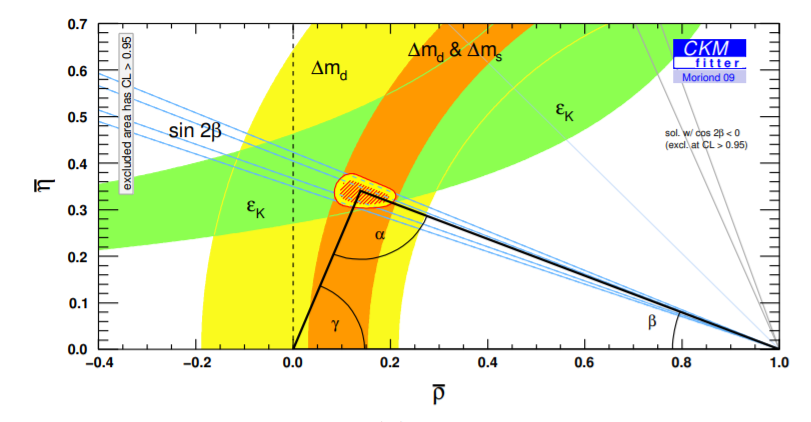
\includegraphics[width=\linewidth]{figures/chapter1/lhcb_goals_b.png}
\caption{Target (Y)}
   \label{plot:plot_triangle_b}
  \end{subfigure}
  \caption[Triangle constraints]{Constraints on the Unitarity Triangle from (a) tree and (b) loop processes, from 2009.}
    \label{plot:both_triangles}
\end{figure}

As can be seen in the \ref{plot:both_triangles}, the constraints on the tree-level before the LHC data taking periods \cite{thelhcbcollaboration2010roadmap} Run 1 and Rub 2  studies were much broader than for the loop processes, which established the need for research in this direction.
The angle calculated by the LHCb for the tree-level decays as of 2020 is $γ = (67 \pm 4)^{\circ}$ \cite{LHCb-CONF-2020-003}.

\section{Test for the lepton universality.}

\begin{figure}
\begin{subfigure}[t]{0.5\textwidth}
  \centering
  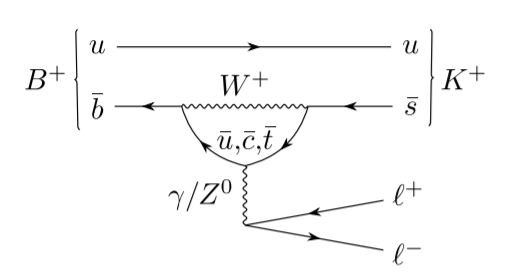
\includegraphics[width=\linewidth]{figures/chapter1/BKLL.png}
  \caption{A decay of $B^{+}$ into kaon and two leptons.}
\end{subfigure}
\begin{subfigure}[t]{0.5\textwidth}
  \centering
  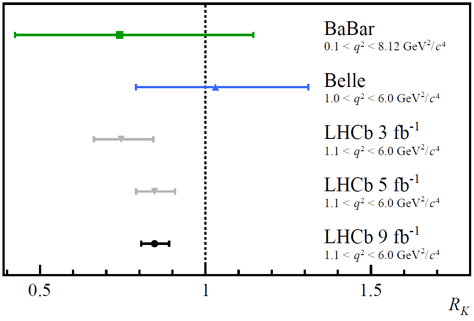
\includegraphics[width=\linewidth]{figures/chapter1/RK2021_s.png}
  \caption{Experimental results of the $R_{k}$ ration calculation.}
\end{subfigure}
 \caption[Experiments]{}
  \label{fig:bkll}
\end{figure}

The coupling of the leptons to the weak gauge bosons is expected to be identical. This is one of the consequences of the Standard Model.
This means that there should be similar decay ratios except for the different masses of the leptons.

The Lhcb collaboration tested this assumption using a $B^{+} \rightarrow  K^{+}\ell \ell $ decay.

As can be seen in the \ref{fig:bkll} process includes a change of the meson $B^{+}$ into kaon by weak force and change of $\bar{b}$ int $\bar{s}$.
The assumption coming from the Standard Model is that the ratios of electrons and muons produced in this process (leptons) should be close to 1. This ratio is called $R_{K}$ and is calculated as $R_{K} = BR(B^{+}\rightarrow K^{+}\mu^{+}\mu^{-})/BR(B^{+}\rightarrow e^{+}e^{-})$


The result of the studies at LHCb is $0.846^{+0.044}_{-0.041}$ \cite{lhcbcollaboration2021test} which is 3.1 standard deviations away from the Standard Model prediction, which hints at the breaking of the lepton universality.
If this result were confirmed with greater confidence, it would suggest new physics beyond the standard model.
%th

\begin{savequote}[75mm]
[..] to unite people from all over the world to push the frontiers of science and technology for the benefit of all.
\qauthor{Cern Mission Statement}
\end{savequote}

\chapter{The Large Hadron Collider beauty experiment}

One of the most famous equations of the modern science: $E = mc^{2}$ states that the energy equals mass (multiplied by the speed of light squared).
The true meaning behind that small equation is immense.
All matter can be changed into energy, and energy can be transformed into matter.
In studies of the elementary particles, this rule is, well, elementary.
If we want all of the different particles of the universe, we can make them, ``just'' by using immense energy.
This energy can take a form of a simple particle (like a single proton), being sped up to great velocities.
If we speed up the same particle but in the opposite direction and subjugate them to collide with each other, the total accessible energy is even greater.
Those collisions produce a vast number of possible particles.
Of course, the more energy there is in a system, the higher the probabilities of creating different states of matter.
This is the reason for the existence of the experimental High Energy Physics as a branch of science.
The Large Hadron Collider was created as a result of a race of reaching ever higher energies.
Furthermore, the Large Hadron Collider beauty \cite{Collaboration_2008} (LHCb) experiment is one of the main experiments that benefit from LHC's particle beam.

\section{Large Hadron Collider}

The LHC (Large Hadron Collider) is probably the biggest machine ever built by humans.
It lies in a circular tunnel beneath the border of France and Switzerland (Geneva).
It is a circular particle accelerator, 27 km in circumference.
The tunnel depth ranges from 60 to 100 meters.

\begin{figure}
  \centering
  \includegraphics[width=0.9\linewidth]{figures/chapter2/CERN_accelerator_complex.jpeg}
  \caption{The entirety of the CERN accelerator complex. (source: \cite{VandenBroeck:2693837})}
  \label{fig:cern_complex}
\end{figure}

The LHC was created in the same tunnel, which housed a Large Electron-Positron Collider.
The accelerator has two beams of particles, the particles used for the beams are usually protons, but heavy ions (i.e. lead ions) are used for some periods of time.
Its actual work was divided into years of runs or data taking periods. Runs 1 and 2 were undergoing in 2009-2013 and 2015-2018. The planned run three is supposed to start in 2022.
% https://news.fnal.gov/2021/11/lhc-is-making-a-splash-as-cms-prepares-for-run-3/#:~:text=On%20Oct.,in%20the%20spring%20of%202022.
There are four main detectors positioned along LHC; Alice, Atlas, CMS, and LHCb.
The entire accelerator complex is depicted in the Fig. \ref{fig:cern_complex}.
The maximal energy of the particles is dependent on the capability of the dipole magnets that are used to guide the particles on the circular path.
As of Run 1 and 2 of the LHC, the dipole magnets could generate 8.33 T  \cite{Evans_2008} for the 7 $TeV$ upper limit energy level of particles.
The maximum energy reached in LHC for a single proton was $6.5 TeV$.
The other set of quadruple magnets is used to create a lensing effect on the particles, which allows to focus the beam correctly.
The beam itself is comprised of bunches of particles.
In order to create collisions, these bunches cross at an approximately $200 \mu \text{rad}$ angle at LHCb \cite{Holzer:1541986}, depending on the energy and conditions.
As seen in the \ref{fig:cern_complex}, the LHC is part of the CERN accelerator complex.
Before the particles make it to the final LHC ring, they are accelerated in stages in pre-accelerators.
For the protons, the first system is a linear particle accelerator LINAC 4, then the Proton Synchrotron Booster (BOOSTER), next the Proton Synchrotron (PS), and finally the last pre-accelerator which is the Super Proton Synchrotron (SPS), which then directly feed the LHC ring.

\section{LHCb spectrometer}

The LHCb\cite{Collaboration_2008} experiment is the main focus of this thesis. It is a single-arm forward spectrometer. Unlike Atlas or CMS, it is not a general-purpose detector although it is sometimes called a general-purpose forward experiment. The initial design focused only on the beauty physics sector, which means studies of the hadrons containing the b-quark. Hence, the ``beauty'' part of the name stands for b quark. In time, its excellent tracking system and flexible high-level trigger allowed to expand significantly the initial physics programme. First, the studies of charmed particles were included, next a number of spectrometry and exotic states searches were added (54 new particles, including penta- and tetra-quarks states, were discovered by LHCb), finally ion and fixed target measurements were performed. The unprecedented precision of obtained results made the LHCb also one of the best place to search for New Physics phenomena. 
The LHCb detector is located underground, in the LHC tunnel, near the french-swiss border on the French side.

The LHCb detector has been undergoing a deep upgrade \cite{CERN-LHCC-2011-001, Bediaga:1443882}, and its composition for the future runs (3 and above) will be different than for runs 1 and 2.
As the scope of this work touches both versions of the detector, the text will mark which detector it refers to, either by date, run or using the word ``upgrade'' to denote the new version of the detector.
Overall, the detector's pseudo-rapidity range is 2 < η < 5, and it's momentum resolution: $Δ p / p = 0.5\%$at low momentum to 1.0\% at $200 GeV/c$ \cite{lhcb_performance_numbers} which is the best at LHC.

\begin{figure}
  \centering
  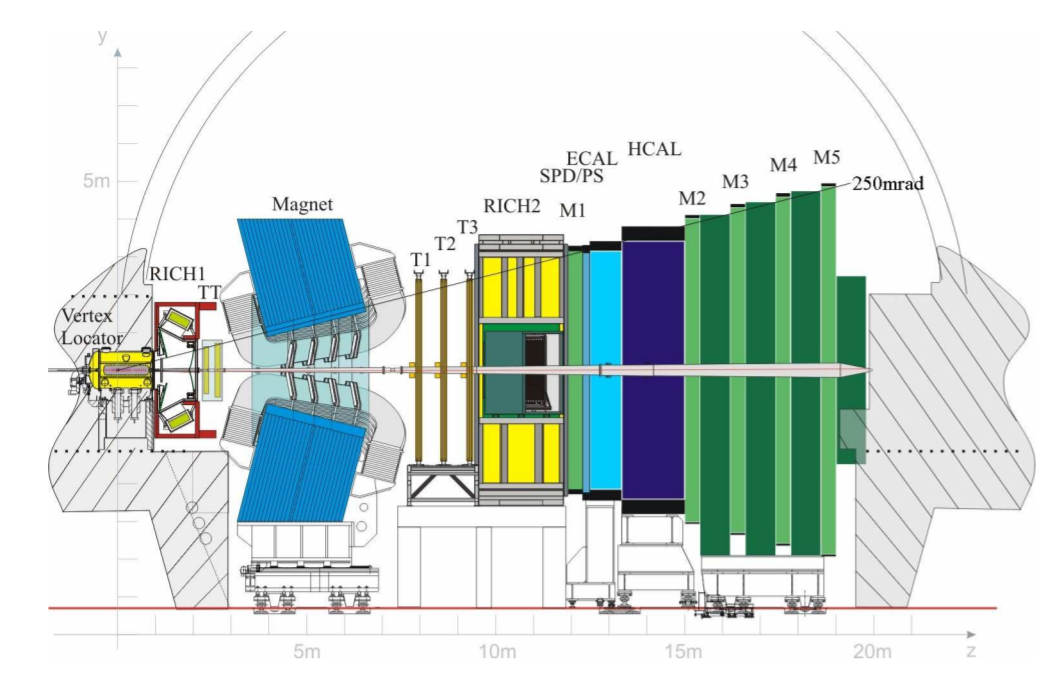
\includegraphics[width=0.9\linewidth]{figures/chapter2/LHCb.png}
  \caption{A cross-section of the LHCb spectrometer in runs 1 and 2, the Velo detector, is visible in the far left of the image.}
  \label{fig:lhcb}
\end{figure}

\section{LHCb subsystems}

This section will briefly discuss LHCb subsystems, apart from the Velo detector, which is discussed in detail in the next section.
The order of the presentation of the subsystems follows their position along the beam axis (see Fig. \ref{fig:lhcb}), that is also the z-axis of the LHCb global coordinate system.

\subsection{Rich}
Ring Imaging Cherenkov detectors (RICH-1 and RICH-2) uses the Cherenkov effect to identify charged hadrons.
RICH-1 is closer to the interaction point and detects lower momentum particles ($~1-60GeV/c$). RICH-2 is downstream after the magnet and is optimised to detect hadrons with momenta in the range ($~15-100GeV/c$)
Both detectors are using different radiation mediums for Cherenkov effect. RICH-1 is using aerogel and $C_{4}F_{10}$, RICH-2 is using $CF_{4}$.
The different media and different Cherenkov angles produced by the particles, with a combination of the momentum information of particle, allow to distinguish protons, kaons and pions with high precision.


\begin{figure}
  \centering
  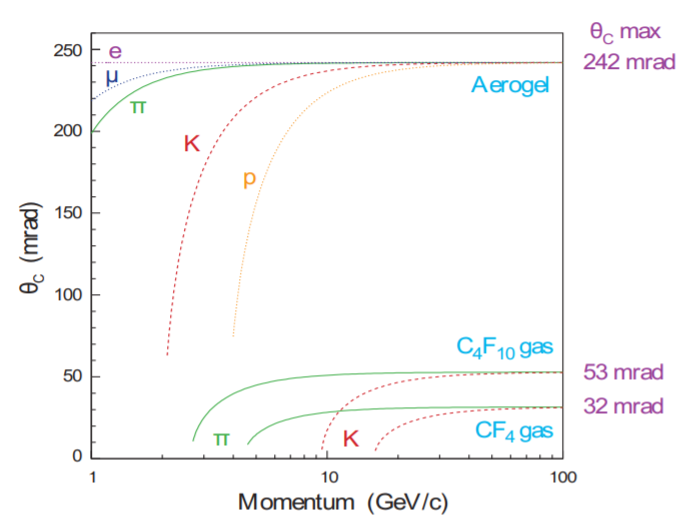
\includegraphics[width=0.55\linewidth]{figures/chapter2/cherenkov_mediums.png}
  \caption{Different media used in RICH with different Cherenkov angles versus their momentum, with different particles.}
  \label{fig:cherenkov_media}
\end{figure}

\subsection{Trackers}
Apart from the Velo, the tracking subsystem can be divided into three parts: Trigger Tracker (TT), Inner Tracker (IT) and Outer Tracker (OT) \cite{Barbosa-Marinho:582793, Collaboration:1647400}.
The IT and TT make up a Silicon Tracker (ST), which utilises the silicon microstrip technology, similar to Velo.
The TT is located upstream and is a 150 cm wide and 130 cm high planar detector between the magnet and the RICH-1 (see Fig. \ref{fig:st_ot}), and the IT station covers a 120 cm wide and 40 high cross-shaped region in the centre of the OT.
The ST was designed with a single hit resolution of 50 $\mu m$
Each of the trackers has four layers which utilise ``xuvx'' topology (two inner layers are rotated by a stereo angle of $+/-5^{o}$, as presented in Fig. \ref{fig:TT}).
The OT is a detector comprising of gas-tight straw-tube modules, with the 4.9 mm inner diameter of the straws. The inner gas is a mixture of Argon (70\%) and $CO_{2}$ (30\%). The gas composition was chosen to guarantee fast drift time  (less than 50 ns) and good drift-coordinate resolution (200 $\mu m$).
It comprises three stations, marked as T1, T2, and T3 in Fig. \ref{fig:lhcb}.
Each of the stations consists of 4 layers employing a similar topology $x-u-v-x$ of the straws, with $+/-5^{o}$ stereo angle.
All of the stations consist of two retractable halves, but unlike the Velo, they are only retracted when servicing.
These halves consist of short modules (S-type) and long modules (F-type).
The F-type modules contain a staggered layout of 256 straws, and the S-type modules containing 128 single straws.
The S-type modules are located closest to the beam and are half of the length of the F-type to compensate for the space for the beam.
In total, there are 168 F-type and 96 S-type modules,

\begin{figure}[H]
\begin{subfigure}[b]{0.45\textwidth}
  \centering
  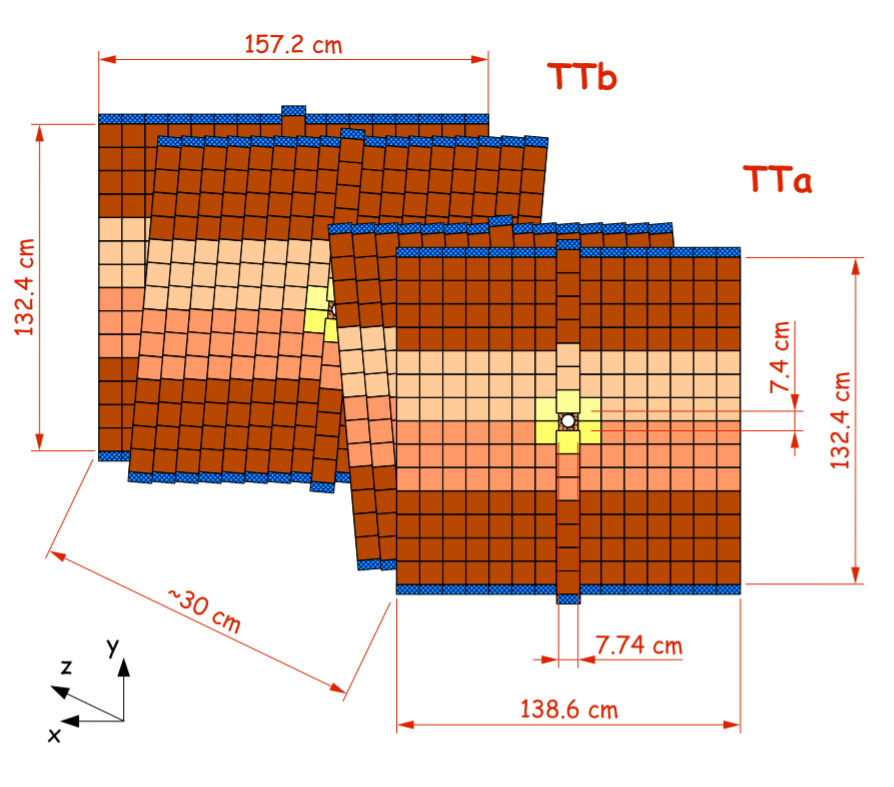
\includegraphics[width=\linewidth]{figures/chapter2/TT.png}
  \caption{TT stations positioning \cite{Knecht:1214889}}
  \label{fig:TT}
  \end{subfigure}
\begin{subfigure}[b]{0.45\textwidth}
  \centering
  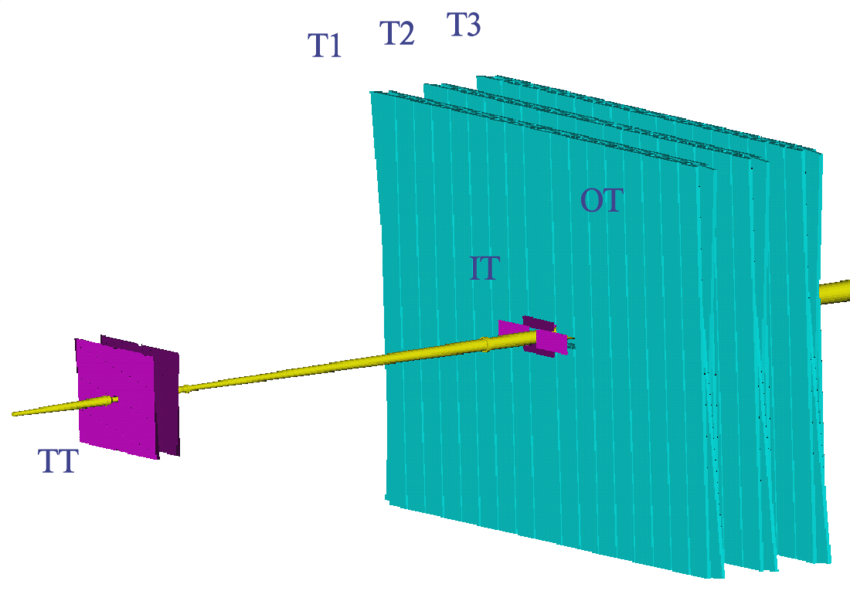
\includegraphics[width=\linewidth]{figures/chapter2/The-main-tracking-system-of-LHCb-TT-IT-and-OT.png}
  \caption{Silicon tracker and outer tracker \cite{alignment-overview}}
  \label{fig:st_ot}
  \end{subfigure}
\end{figure}

\subsection{Magnet}

Next to the TT stations, depicted in blue at Fig. \ref{fig:lhcb}, there is a massive warm, dipole magnet of 1600 tonnes of weight between the tracking stations. Its purpose is to bend the charged particles' trajectory to determine their charge and momentum.
High performance LHCb tracking system requires that the field generated by the magnet has to be carefully mapped with the precision better than $0.1$ \textperthousand.


\subsection{Calorimeters}
The calorimeter system at LHCb consists of three components: PS/SPD (preshower detector/scintillator pad detector), ECAL (electromagnetic calorimeter) and HCAL (hadronic calorimeter).
There are two common types of showers in the calorimetry world: electromagnetic showers and hadronic showers.
When the electron or positron enters scintillating active material, it emits a photon.
A photon, in turn, dissociates to an electron-positron pair, which creates a positive feedback loop that creates more and more particles.
This is known as an electromagnetic particle shower and is depicted in Fig \ref{fig:em_shower}.

\begin{figure}[ht]
  \centering
  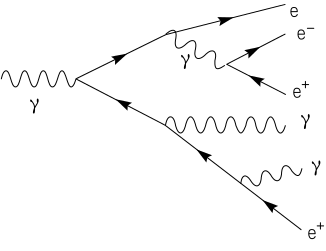
\includegraphics[width=0.35\linewidth]{figures/chapter2/Schematic_of_a_particle_shower.svg.png}
  \caption[something]{Exemplary graph with electromagnetic particle shower\footnotemark. }

  \label{fig:em_shower}
\end{figure}

\footnotetext{ Image source: \url{https://commons.wikimedia.org/wiki/File:Schematic_of_a_particle_shower.svg} }

The hadronic particle shower is more complicated and involves interaction via the strong force.
The electromagnetic calorimeter was created for the purpose of capturing electromagnetic showers.
The rejection of the high-energy charged pion showers in the ECAL requires a PS detector placed in front of the ECAL.
Furthermore, neutral pion showers also must be rejected. For this reason, the SPD detector was positioned in front of the PS detector, separated by a lead converter.

The electromagnetic shower is induced more easily and is shorter than the hadronic one.
The HCAL is much denser and bigger to allow for complete deposition of the energy of the hadronic shower.

\subsection{Muon station}

\begin{figure}
  \centering
  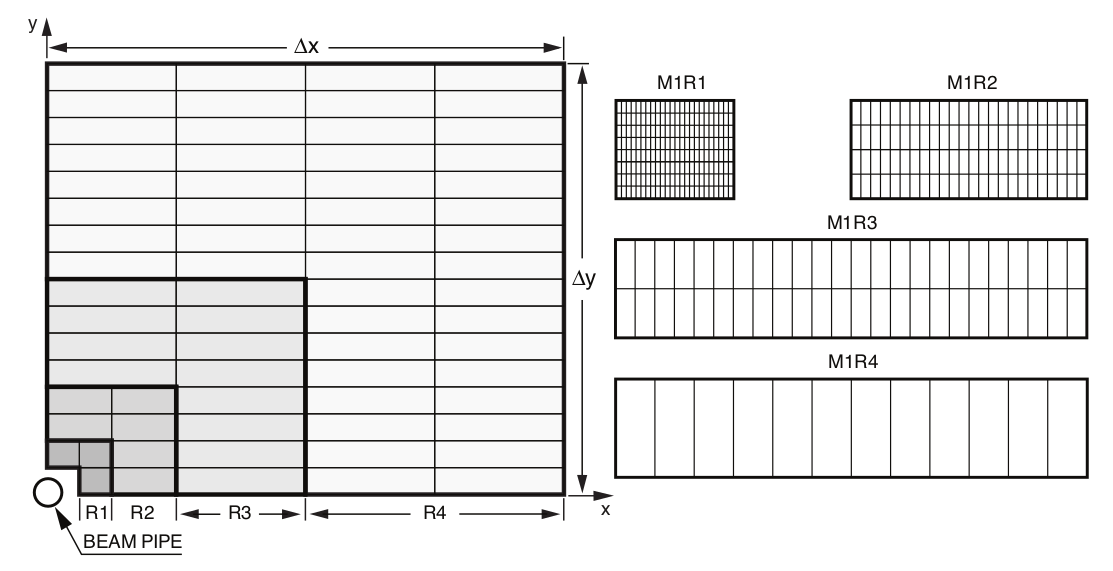
\includegraphics[width=0.9\linewidth]{figures/chapter2/muon_system_partition.png}
  \caption[somethingelse]{Left: front view of a quater part of the muon station, each part reperesents a single region (R1, R2, R3, R4). Right: Division of the each of four region chambers into logical pads.} 

  \label{fig:muon_partition}
\end{figure}

The muons are about 200 times heavier particles than the electrons and exhibit much less energy deposition in matter. In a typical case muon detectors are positioned at the outermost part of the setup (this is the case for LHCb spectrometer). Muons, thanks to their properties constitute a very convenient objects to trigger on. 

In LHCb, the muons system consists of five stations (M1-M5). It is a gas detector consisting of a total of 1380 chambers.
The stations M2-M5 are positioned downstream, and between each station, there is an iron absorber 80 cm thick.
All of the stations utilise MWPC (multi-wire proportional chambers) technology, except for the inner region of the M1 station, which uses triple-GEM (gas electron multiplier) detector chambers.
All stations are divided into four regions, R1, R2, R3, and R4, corresponding with the 1:2:4:8 ratio of length from the beam (as seen at \ref{fig:muon_partition}).
The inner space of MWPC is filled with a mixture of $Ar/CO_{2} /CF_{4}$ (40 : 55 : 5), and contains a wire plane of 2 mm spacing, symmetrically placed in a 5mm gap. This allows for 5ns time resolution.
Each chamber consists of four gaps with wires.


\section{Velo}

The Velo detector (Vertex Locator) is the heart of the LHCb spectrometer.
Its main goal is to record the charged particles' trajectory and reconstruct the collision point with extreme precision. As mentioned in the previous section, the composition of the LHCb spectrometer is changed in upcoming Run 3. The Velo detector is (as of the time of writing) being upgraded from a silicon micro-strip detector to a silicon pixel matrix detector. Because of the possible confusion I assumed the following naming convention throughout my Thesis. I will refer to the upgraded detector as ``VeloPix'', and to the detector used in Run 1 and Run 2 as  ``Velo Strip'' or simply ``Velo''. The readout chip is called VeloPix ASIC or VeloPix chip.

\subsection{Strip Velo in Run 1 and 2}

The Velo in the Run 1 and 2 consists of 42 modules.
Each of the modules is comprised of 2 sensors: $R$ and $\phi$-type.
Each sensor side is a silicone microstrip sensor.
The individual sides correspond to different polar coordinates, as depicted at Fig. \ref{fig:velo_routing}.
Each sensor had 2048 silicon strips (physical channels).
In total, it gives more than 170 000 strips in the entire Velo detector.


\begin{figure}[H]
  \centering
\begin{subfigure}[t]{0.7\textwidth}
  \centering
  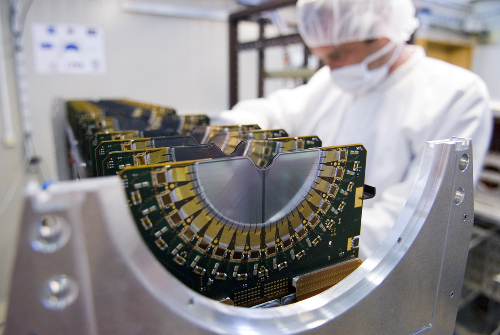
\includegraphics[width=\linewidth]{figures/chapter2/velo_assembly.jpg}
  \caption{Strip Velo during assembly\footnotemark. }
  \label{fig:velo_assembly}
  \end{subfigure}
\begin{subfigure}[t]{0.7\textwidth}
  \centering
  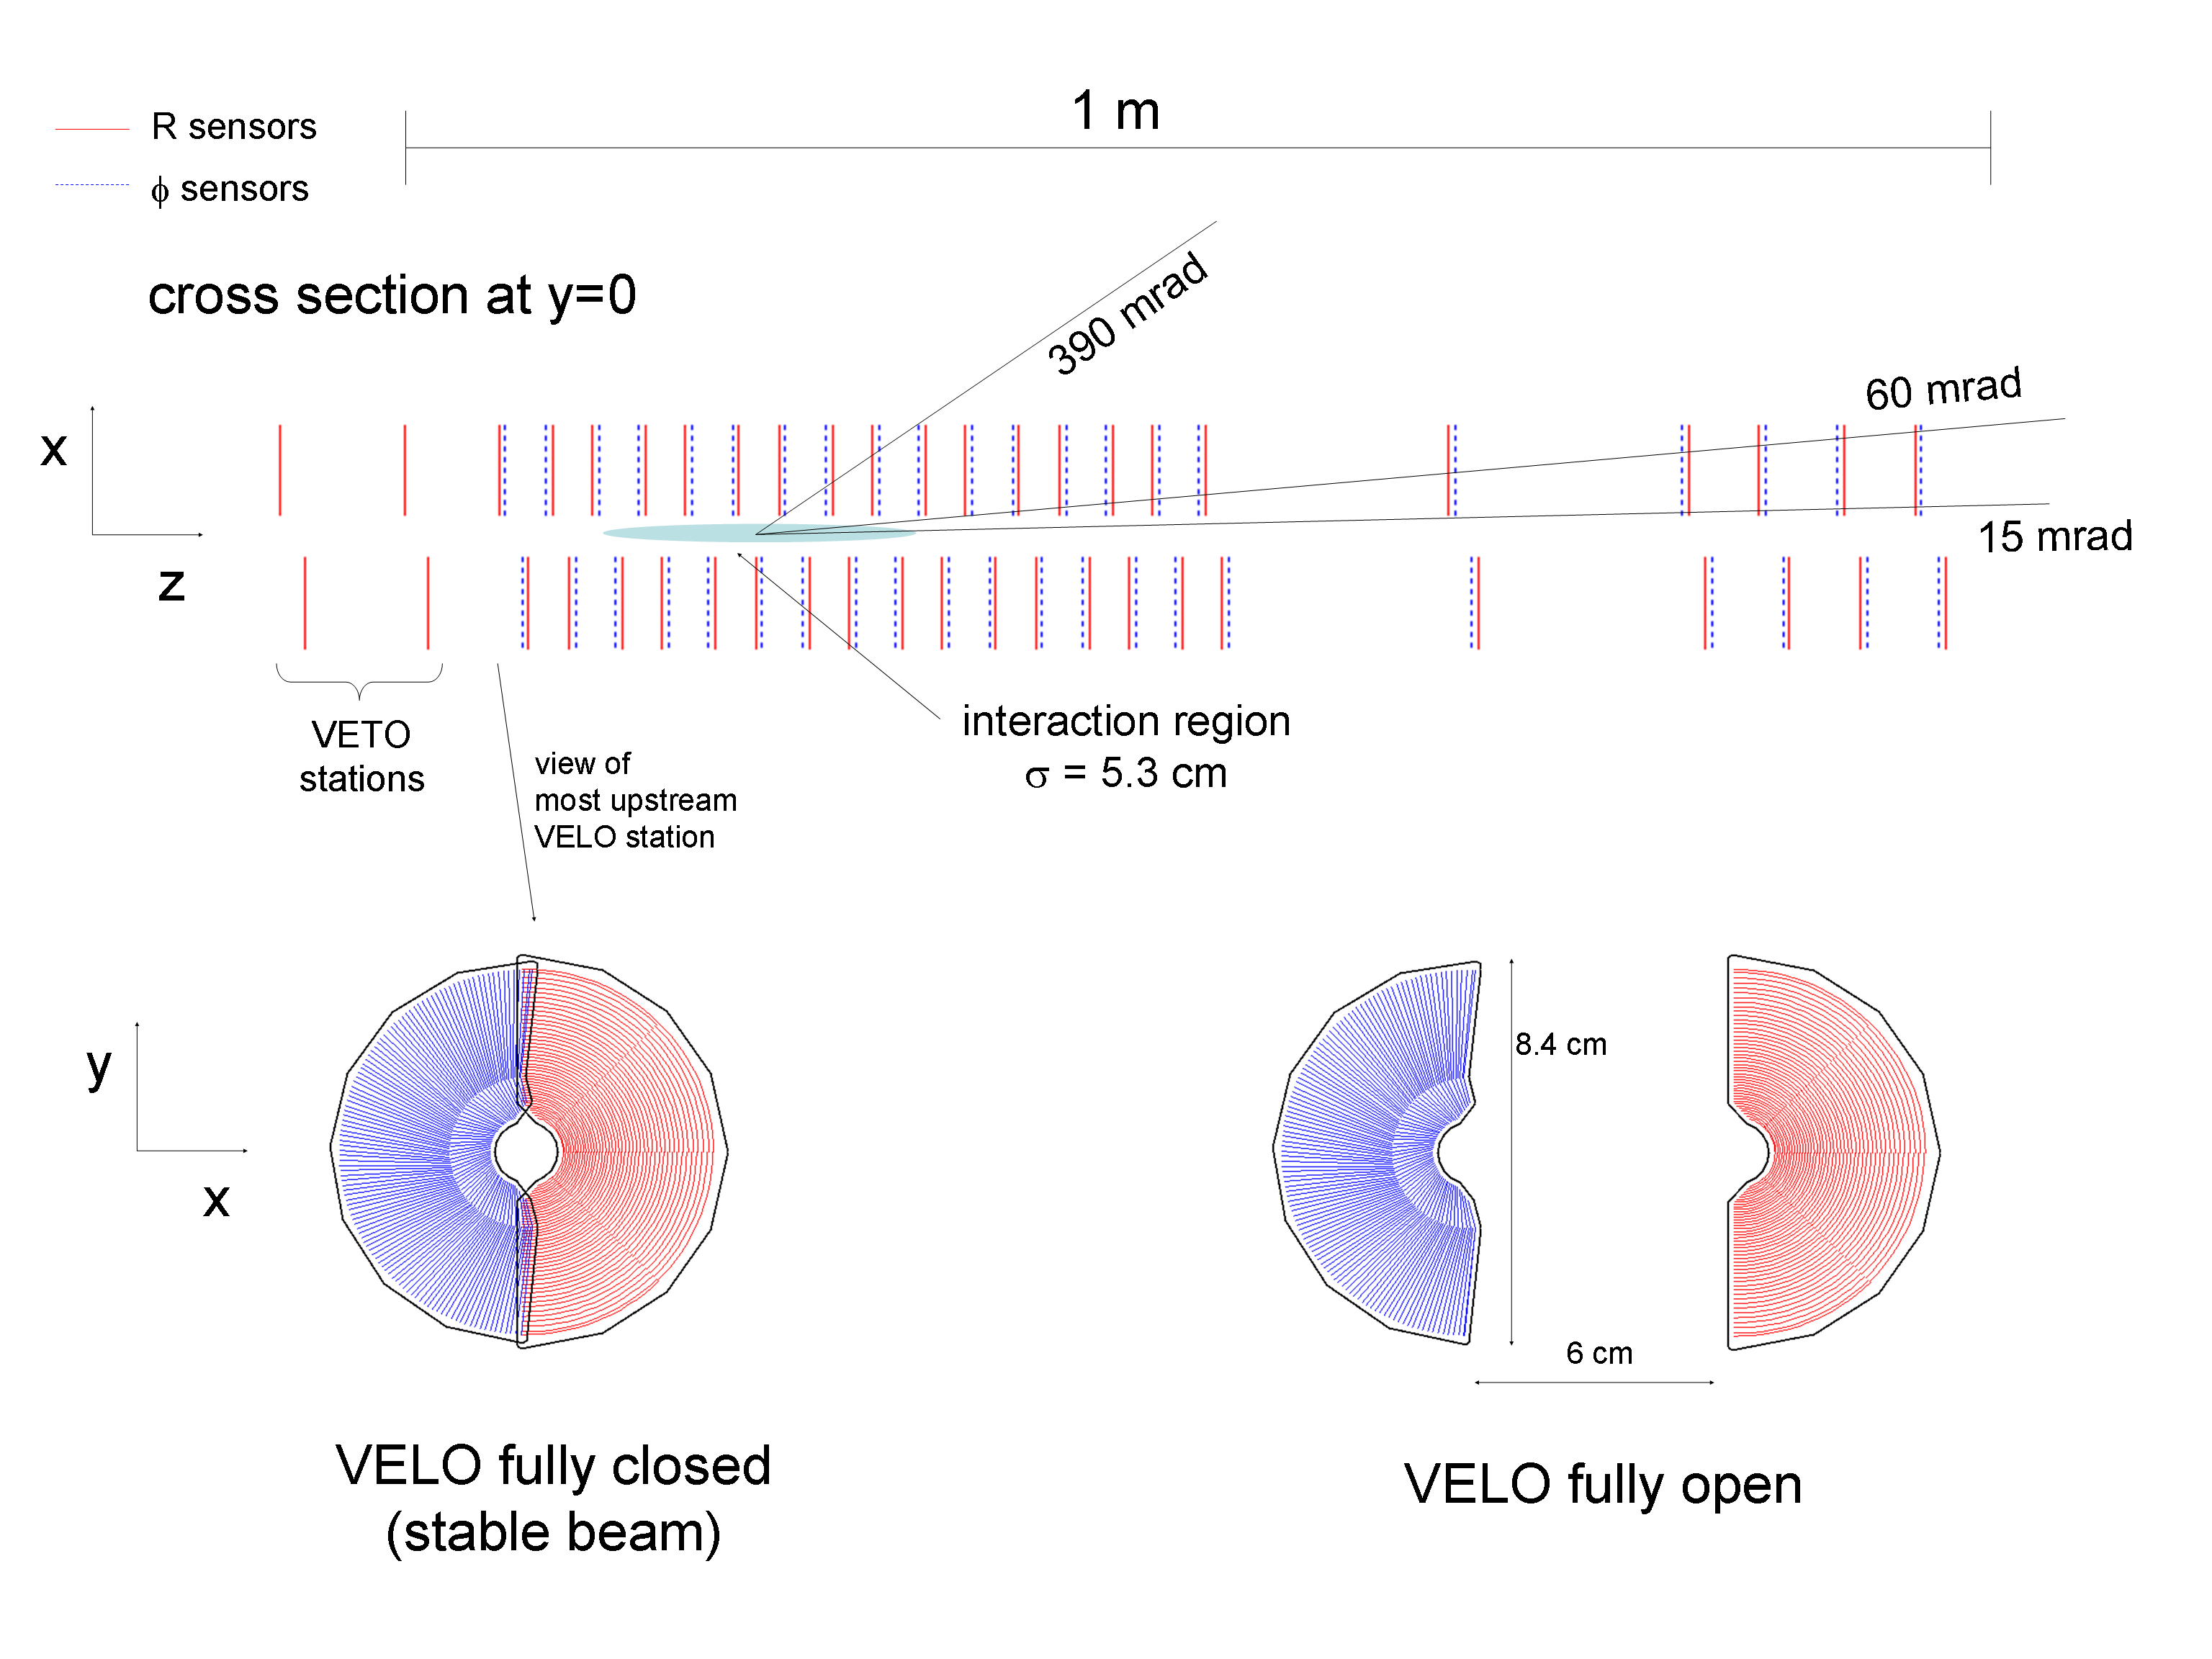
\includegraphics[width=\linewidth]{figures/chapter2/veloOverview.png}
  \caption[overview]{Overview diagram showing the spacing of modules along Z and positions open and closed.}
  \label{fig:velo_overview}
  \end{subfigure}
\end{figure}

\footnotetext{ Image source: \url{ https://lbtwiki.cern.ch/bin/view/VELO/VELOConferencePlots} }

Velo modules are mounted on two retractable halves, which enclose the beam. The movable construction is necessary to protect the LHC beam during the injection stage, before the stable beam condition is achieved.
One of the halves is visible in the Fig. \ref{fig:velo_assembly}.
The alignment of the modules on the halves is staggered as depicted in Fig. \ref{fig:velo_overview}.
Additionally to 42 two-sided modules, four VETO stations are positioned on the other side of the interaction point, consisting of only R-type sensors. The VETO stations proved very useful to provide information to the trigger system and measure the rapidity gap.

The Velo detector (both Velo Strip and VeloPix) is enclosed in its own secondary vacuum tank, which is separated from the primary beam vacuum.
The geometry of the inner gap of sensors is 8mm in radius, and the outer radius of the sensor is about 42 mm.
When the stable proton beam is decalred, the halves of the detector are being retracted (so called closing procedure), which requires the precise position of the collision point to be calculated.
After that, the halves of the Velo detector are moved closer gradually towards the beams using stepper
motors. Sensors get as close as 7 mm to the interacting beams. \cite{Aaij:1707015}.
The sensors themselves are created using oxygenated $n^{+}$-on-$n$ technology, consisting of $n^{+}$-type implant on a $n$-type bulk with a back-plane of $p^{+}$-type implant.
With an exception for two most upstream modules that where produced using the $n^{+}$-on-$p$ silicon type.

The sensors are 300 $\mu m$ thick, and their spatial separation (pitch) varied as a function of radius \cite{Barbosa-Marinho:504321} as depicted on the \ref{fig:velo_pitch}. The way that physical sensor strips were arranged, with their routing lines, influences the ordering of the data and the calibration procedure.

\begin{figure}
  \centering
  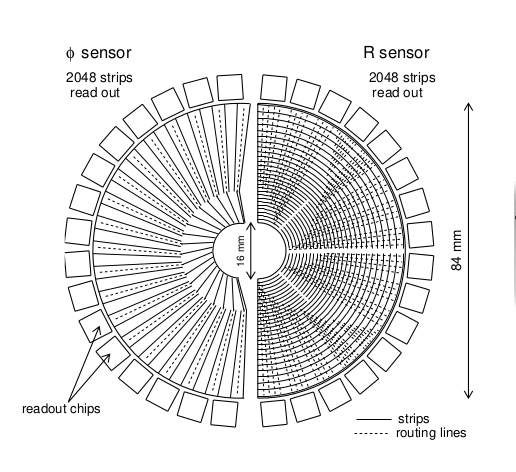
\includegraphics[width=0.7\linewidth]{figures/chapter2/velo_module_routing.png}
  \caption{A depiction of Velo sensors and their routing lines.
    This is just the schematic representation as it does not reflect the actual number of strips and routing lines.
    The $\Phi$-type sensors' outermost strips are directly connected to the readout chips without a need for long routing lines, but the innermost part has routing lanes lying parallel to the outermost strips.
    The $R$-type sensor routing is divided into sections of routes with different lengths.
    In reality, both sensors are divided into 512 long sections of repeated routing lines lengths.
  }
  \label{fig:velo_routing}
\end{figure}

\begin{figure}
  \centering
  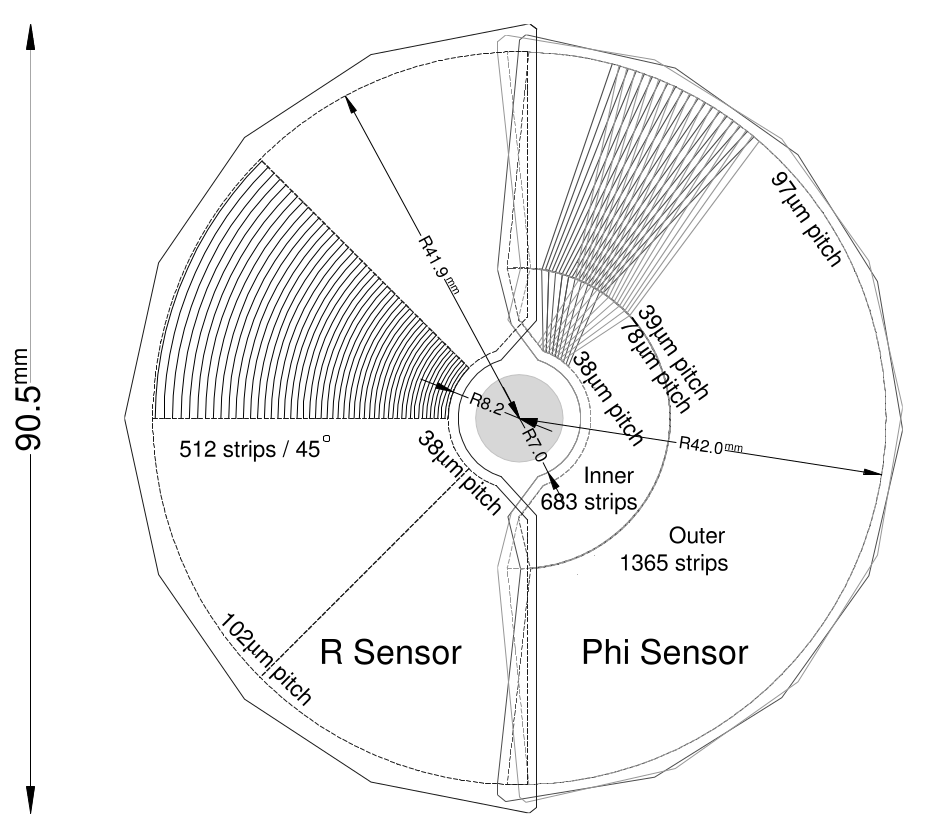
\includegraphics[width=0.7\linewidth]{figures/chapter2/velo_module_pitch.png}
  \caption{ A detailed view of the Velo sensors with their according pitch. The R sensor's pitch starts at 38$\mu m$ and ends on 102$\mu m$. The $\Phi$-type sensors' pitch modulation is divided in two. The most inner 683 strips have from 38 $\mu m$ to 78 $\mu m$ pitch, and the outer rest has a pitch ranging from 39 $\mu m$ to 97 $\mu m$. }
  \label{fig:velo_pitch}
\end{figure}


As seen in the Fig. \ref{fig:velo_routing}, the ordering of the R-type sensor routing lines is divided into four sectors and varies in the distance of the strip from the centre (proton beam). What is not visible in the Fig. \ref{fig:velo_routing} (because of the simplification of the plot) is that the $\Phi$-type sensor is also divided into two parts (as seen in the \ref{fig:velo_pitch}).

The silicon strips are connected to the Beetle front-end ASICs that are mounted on the Velo module board.
Each Beetle chip has 128 indivudually instrumented readout channels. In the case of Velo the signals read from the detector are only conditioned by the analogue part of the chip and send via 60 m long copper cables for digital processing to the electronics Tell1 boards. 
The strips are sampled with 40 MHz frequency and internally queued \cite{Löchner:1000429} in an analogue pipeline.
The analogue data are brought off-chip at 1.1 MHz, with 32 channels multiplexed over four lines.

As mentioned above, the data readout from the Beetle chips was passed to Tell1 boards.
The Tell1 boards have been standardised for the entirety of the LHCb detector.
They accept either optical or analogue receiving cards.
The information was then processed on the on-board FPGAs with custom processing algorithms.
From the Tell1 electronics, the data was transferred to higher-level systems like ECS (Experimental Control System) and triggers.

\subsubsection{Calibration procedure for Velo}
\label{chap2:calibration}
% http://cds.cern.ch/record/1074928/files/lhcb-2007-151.pdf
% https://inspirehep.net/files/83cebd5d85f3494474861bf522e0bbb9
In the absence of proton-proton collisions, the signal observed on each Velo readout channel is approximately normally distributed.
In the first place, the calibration procedure aims to shift the central value of each of these distributions to zero (so called base-line correction).
As shown in the top plot in Fig. \ref{plot:postcal} this offset (also called the pedestal) is, in general, different for each individual channel and needs to be evaluated by a dedicated algorithm using RAW Non-Zero Suppressed Velo data taken without colliding beams.
The equalised Non-Zero Suppressed data are shown at the bottom of Fig. \ref{plot:postcal}.
After the offset correction is applied (called the pedestal $P$ subtraction,\cite{Aaij:1707015}) the noise can be estimated in each channel as the width of the signal distribution.

\begin{figure}
    \centering
    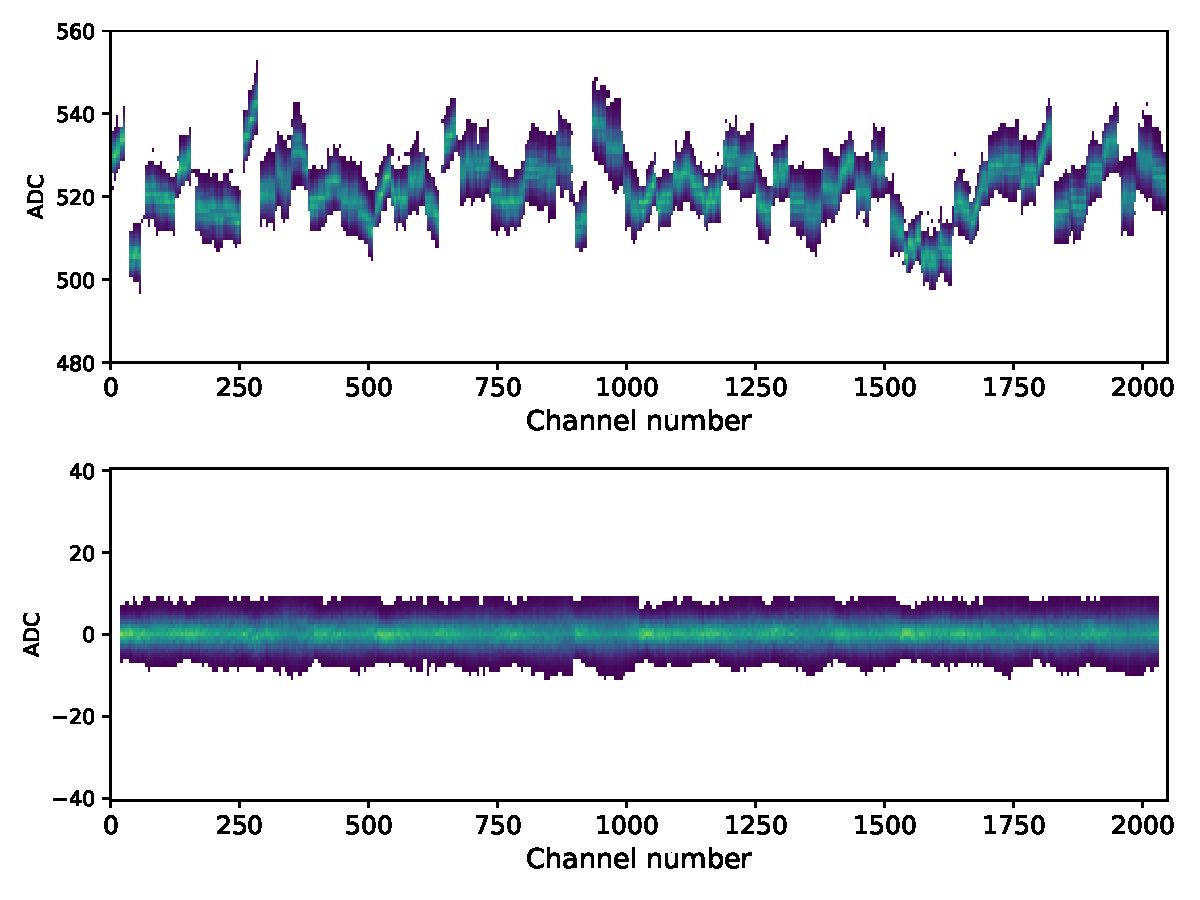
\includegraphics[width=0.7\linewidth]{figures/chapter2/pre_post_cali.pdf}
    \caption[thing]{Typical RAW Non-Zero Suppressed Velo data before (top) and after the digital processing (bottom). The response of each channel was equalised, and a common flat baseline centred on 0 ADC\footnotemark achieved. The spread of the data points about the baseline is attributed to the total noise present in the system.}
    \label{plot:postcal}
\end{figure}

\footnotetext{Where ADC is Analogue to Digital Count that represents the amplitude of the signal after the digitisation.}

The noise evaluated during the calibration procedure is vital for the hit detection and cluster reconstruction algorithm since it is used to suppress the channels without high ADC counts (Zero Suppression procedure). Here, we assume the correlation between charged particles passing through sensors and depositing the energy in their active volume and the signal amplitude measured on each readout strip.
The performance of the cluster reconstruction  algorithm is of critical importance for the Velo data quality.
The algorithm is comprised of two stages hit detection and cluster building.
The former step relied on so-called high thresholds evaluated for each channel using the measured noise.
For each channel, the high threshold, $H_t$, was set to be five times higher than the noise measured on this channel.
Taking into account the approximate Gaussian nature of the signal distribution without particle hits, it corresponds to the probability of accepting a noise signal as a real hit at the level of $10^{-7}$.
The cluster building step used the selected channels that passed the hit detection algorithm as seeds.
Clusters were formed by searching for the secondary signal channels using so-called, low hit thresholds.
Up to four channels were used to form a single cluster.

In general, the clustering algorithm works as follows\cite{Parkes:1074928}:
\begin{enumerate}
  \item If the measured signal exceeded the high threshold $H_{t}$ on strip $S_{n}$, then the channel was tagged as the cluster seed.
  \item In the next step, the signal measured on the adjacent strips, with respect to a seeding strip, were compared to the low thresholds. All strips that passed the low threshold cuts were tagged, along with the seeding strip, as a cluster candidate
  \item In the last step, a cluster (hit) was built. A global cut on the cluster size was set to four strips. In case when a cluster candidate is comprised of more strips, the algorithm creates multiple adjacent clusters. Finally, the local position of each created cluster was evaluated using a centre of gravity formula.
\end{enumerate}

A visualisation of the algorithm can be found in the Fig. \ref{plot:velo_clustering}.

\begin{figure}
    \centering
    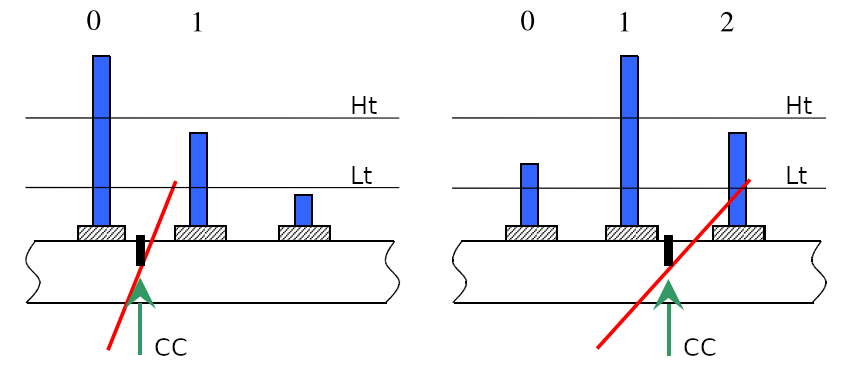
\includegraphics[width=0.7\linewidth]{figures/chapter2/clustering_algorithm_velo.png}
    \caption{Visualisation of the clustering algorithm. Two examples of Velo clusters are shown schematically. Blue rectangles depict the charges collected on the strips. Black lines represent high threshold $H_{t}$ and low threshold $L_{t}$ cuts, the reconstructed cluster centre (CC) is indicated by arrows and the particle trajectory is given by the red sloping lines.}
    \label{plot:velo_clustering}
\end{figure}

\subsubsection{Header Cross-Talk}
\label{chap2:headercrosstalk}

The Beetle chips in Velo are connected to 128 physical strips and send data on four analogue links, with 32 channels of analogue data.
There is a pseudo-binary information header preceding the analogue data.
This information consists of four bits and encodes the status of the front-end chips and the pipeline column number.
Unfortunately, this caused a problem in the data transfer, and the four preceding bits induced an additional noise in the first upcoming data channel.
In total, this contributed to the increased noise in 64 channels in Velo sensor.
This effect is known as header cross-talk\cite{Szumlak:1177860}. The initial commissioning studies, performed before Run 1, showed that this can produce a significant stream of fake clusters increasing the volume of the Velo data transmitted to the high-level trigger. A dedicated correction algorithm has been developed in order to alliviate the problem.

\subsubsection{Voltage and luminosity}
\label{chap2:lumivolt}

Each of the strips in Velo is, in essence, a semiconductor diode. It is an $n^{+}$-type implant in an n-type bulk with a back p-type implant\cite{Akiba:2633496}.
The physical process of exciting the matter electromagnetically inside the sensor bulk creates a cloud of electrons and holes.
For the charge to be able to cross the depletion region, there needs to be additional bias voltage applied.
This is also a way of mitigating the radiation damage, as the multiple negative factors disrupt the flow of the generated charge.
The Fig. \ref{fig:radiation_damage}, shows that the bias voltage necessary for the optimal operation of the Velo detector has been steadily growing along with the delivered integrated luminosity.

\begin{figure}[H]
  \centering
\begin{subfigure}[t]{0.654\textwidth}
  \centering
  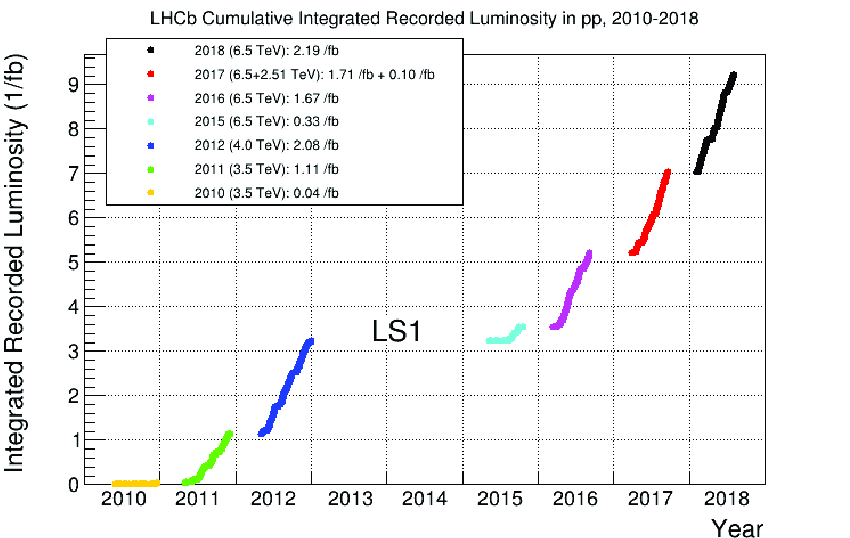
\includegraphics[width=\linewidth]{figures/chapter2/LHCb-Cumulative-Integrated-Recorded-Luminosity-in-pp-2010-2018.png}
  \caption{Integrated luminosity for the years 2010-2018 \cite{Kurbatov}.}
  \label{fig:velo_lumi}
  \end{subfigure}
\begin{subfigure}[t]{0.65\textwidth}
  \centering
  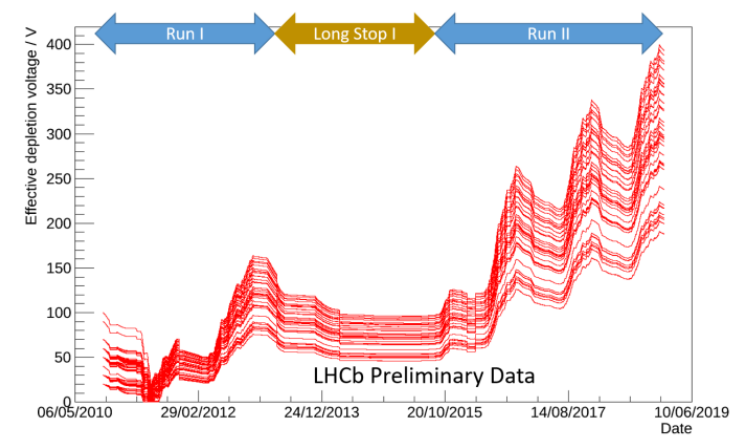
\includegraphics[width=\linewidth]{figures/chapter2/velo_strip_voltage.png}
  \caption[stripvo]{Projected Velo bias voltage.}
  \label{fig:velo_voltage}
  \end{subfigure}
  \caption[]{Radiation damage effects on the LHCb Velo.}
  \label{fig:radiation_damage}
\end{figure}


\subsection{Velopix}

The Large Hadron Collider and its detectors were planned to be incrementally
improved over time. In LHC Run 3, there will be a significant increase
in the instantaneous luminosity, and the Velo must adapt to that change. For this purpose the Velo group proposed to change the sensor technology from planar strip sensors to pixel ones
read-out by the VeloPix ASIC that was adapted from the TimePix chip.

Some of the requirements for the upgraded detector include:
\begin{itemize}
\item \textbf{Increased rate of data} output to 40 MHz with hits/event $≈ 5.2cm^{-2} \times R^{−1.9}$ (R is radius in $cm$).
This means that the VeloPix ASICs must be able to output up to 15.1 GB/s. The peak total data rate of upgraded Velo can reach up to 2.85 Tbit/s.
\item \textbf{Irradiation} the upgraded detector is predicted to experience an accumulated the flux of fast hadrons
$∼ 8 \times 10^{15}n_{eq} /cm^{2}$, and when this is reached, it is expected that the bias voltage and the current necessary for operating the sensors at the pixel closest to the beam will be $1000V$ and $200 \mu A/cm^{2}$ at -20C.
Such a high dose of radiation and high currents will make a significant obstacle in protecting the sensor from thermal runaway.
\end{itemize}


\begin{figure}
  \centering
  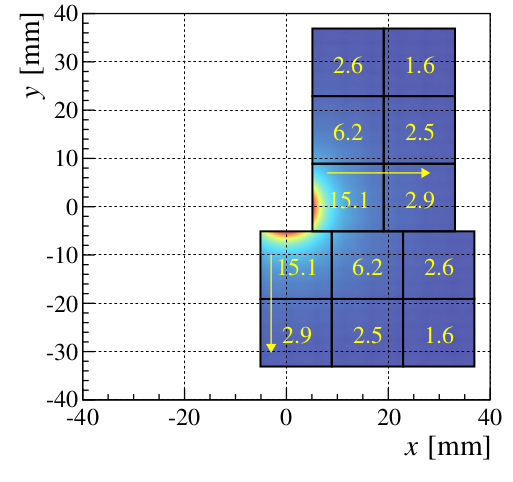
\includegraphics[width=0.4\linewidth]{figures/chapter2/data_rate.png}
  \caption{The projected data rate for each ASIC in Velo module (in Gbit/s).}
  \label{fig:velopix_datarate}
\end{figure}
\begin{figure}
  \centering
  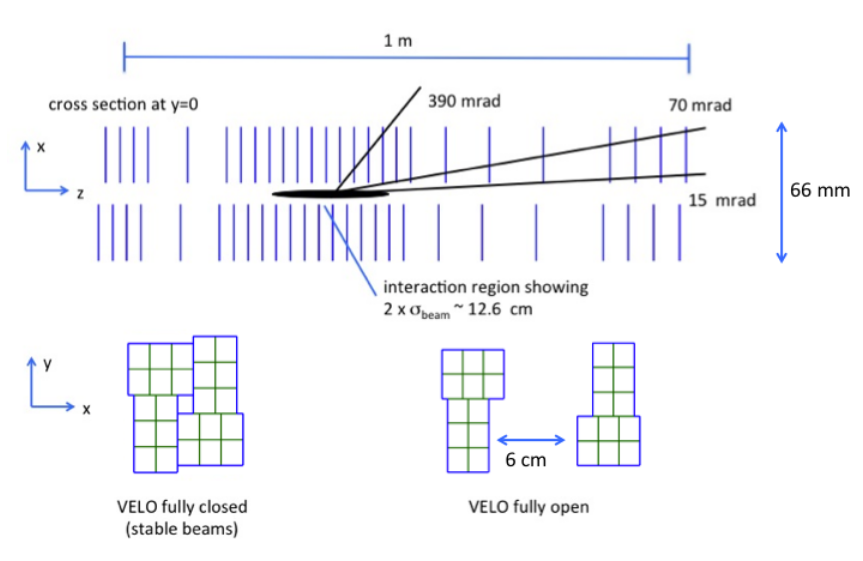
\includegraphics[width=0.7\linewidth]{figures/chapter2/velopix_layout.png}
  \caption{  }
  \label{fig:velopix_layout}
\end{figure}

The new upgraded Velo detector that will collect data during Run 3 and Run 4 has a modular design, similar to the previous strip device. Each module contains 4 sensors, each sensor is readout by
3 VeloPix ASICs. VeloPix chips are rectangular in shape and can readout matrices of 255x255 pixels.
New Velo sensors feature square $55 x 55 \mu m^{2}$ pixels that provides excellent spatial resolution. 
There are 52 modules arranged along the z-axis (i.e., along the LHC beam). It is worth noticing that significant portion of the Velo strip detector's infrastructure remained, for instance the secondary vacuum tank.
A simplified visualisation of the Velo modules z-positions and the pixel sensors geometry is shown in Fig. \ref{fig:velopix_layout}.

In order to process the data more effectively and save the transmission bandwidth individual pixels are grouped on the logical level in, so called, super-pixels.
Super-pixels consist of eight pixels arranged as 2 by 4 matrices.
Sending data using the super-pixels instead of pixels allows for a reduction of the total required bandwidth by about 30\% \cite{Collaboration:1624070}.
When there is a hit in the super-pixel, a 9-bit timestamp is created and stored.
Each super-pixel can store up to two timestamps.
Readout from the super-pixels is done via a 23-bit bus running at 13.3 MHz.
This means that there is a data transfer only when there is a hit information. In other words, the new VeloPix detector is a trigger-less system.

\subsubsection{Velopix masking and calibration}
\label{chap2:velopix_calibration}

A critical functionality of both vertex systems is a possibility to deactivate a problematic readout channels, also called "bad" channels. Typical reasons for deactivation can be related with sensor issues (for instance physical damage), problems with bonds (broken bond or partially connected bond) or readout lines. The best strategy to identify bad channels is to measure and trend noise.
The procedure of collecting the noise data (without proton-proton collisions), identifying problematic channels and then disabling them is called masking. During the Run 1 and Run 2 operation a significant experience was gained related to this important issue. There was a fraction of bad channels that were considered "fixed" and they do not changed over time, however, a majority of them did not show permanent problems and evolved in time. Quick tagging of bad channels was essential for keeping the high data quality. For instance, a large number of noisy channels will create a stress in trigger readout system by producing spurious fake hits. This may degrade the tracking and increase processing time due to larger number of hits. In case of the pixel detector, that operates in trigger-less mode, large number of unmasked noisy channels can completely saturate the readout lines, since the fake hits will be sent constantly (in case of the strip detector it would be just one fake cluster per one trigger). Evaluation of the set of pixels to be masked will be performed during the, so called, equalisation that is the core of the VeloPix calibration procedure. The number and distribution of the masked channels must be carefully study and monitor during the data taking period. A short description of the equalisation is given below.





\begin{figure}
    \centering
    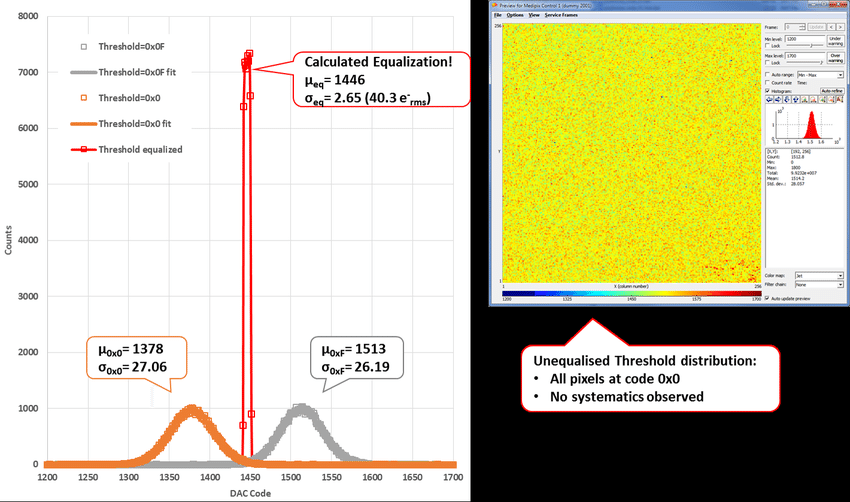
\includegraphics[width=0.7\linewidth]{figures/chapter2/Threshold-spread-in-the-pixel-matrix.png}
    \caption{Exemplary threshold spread of the pixel matrix.}
    \label{plot:velopix_thresholding}
\end{figure}

% https://lbtwiki.cern.ch/bin/view/VELO/VeloUpgradePresentationMaterial
% @TODO add images

% https://www.researchgate.net/publication/312869714_The_VeloPix_ASIC // \cite{poikela}
% https://www.researchgate.net/publication/224577931_Optimization_of_Medipix-2_Threshold_Masks_for_Spectroscopic_X-Ray_Imaging#pf5
% http://cds.cern.ch/record/2636158/files/VeloPix%20Data%20Visualisation%20and%20Read-out%20Control.pdf
% https://cds.cern.ch/record/2723996/files/2006.09559.pdf
% https://www.researchgate.net/publication/291436661_Equalization_method_for_Medipix3RX

Similarly to strip Velo, VeloPix will collect the noise calibration data \cite{Kopciewicz:2723996}. In
the case of the VeloPix, each pixel has its own individual voltage threshold. If this
threshold is exceeded by signal induced by a passing charged particle, we register a hit.
There are two types of values that can be set in a readout chip to define individual thresholds: Global Threshold (GT) and Trim.
The former is evaluated for each sensor matrix (255 x 255 pixels), whilst, the latter are defined per individual pixel,  they are 4-bit numbers (16 different values).
Trim is a readout DAC voltage that is individually added to the signal in the discriminator such that it allows to achieve equal response for each pixel across the whole detector matrix.
For the convenience of the Reader, the automatic procedure that is used to evaluate the GT and Trims is described briefly below.
First, we set all pixels to use their $Trim_{0}$ value, and we scan the reaction of
the pixels (thresholds) by moderating $GT$ value and, each time opening the shutter for a constant
amount of time $T_{C}$. Then we repeat this operation for $Trim_{15}$.
In both trim cases, we record the total number of active pixels (pixels that registered noise)
$N_{HITS}(GT)$ as a function of $GT$, as well as the number of registered hits ${H_P}_{x,y}(GT)$ in each
pixel $P_{x,y}$, in a $GT$.
The mean of the gaussian distribution of noise events $H_{P_{x,y}}$ for each of the steps of $GT$ is
used to calculate lower bound for trim ${TrimValue_0}_{x,y}$ in case of
$Trim_{0}$, as well as to calculate ${TrimValue_{15}}_{x,y}$ in $Trim_{15}$.
That means that a scan in $Trim_{0}$ and $Trim_{15}$ is used to set the range of voltage for
the trims.
The ${TrimValue_{0}}_{x,y}$ is used as the lower bound for all of the 16 trims in
each individual pixel and the ${TrimValue_{15}}_{x,y}$ is used as the maximal bound for the trims.  Therefore one step of the trim is
$TrimStep_{x,y} ={TrimValue_{15}}_{x,y}-{TrimValue_{0}}_{x,y}/15 $.

That process allows us to calculate and calibrate trim values for each pixel.
Now to determine which of the trim value should be set for the pixel, we
take advantage of the $N_{HITS}(GT)$ measured in each of the two scans ($Trim_{0}$ and $Trim_{15}$). Both of those
yield noise events distributed normally.
We calculate mean of the distribution in TRIM0 $M_{TRIM0}$, and TRIM15
$M_{TRIM15}$. The final value of the trims is calculated as
$GT_{target} = M_{TRIM0}+M_{TRIM15}/2$.
Then each of the pixels gain the trim value of ${PixelTrim_{x,y}}_{a}$ set as close to
$GT_{target}$.
Then to exclude the noise from the signal coming from the pixels, the
effective global threshold $GT_{effective}$ is set to
$GT_{target} + 1000 electrons$.
So the actual threshold for the individual pixel
$Th_{x,y} = {PixelTrim_{x,y}}_{a} + GT_{target} + 1000 electrons$
This procedure is visualised in Fig. \ref{plot:velopix_thresholding}.
% \subsubsection{Calibration example}
% Let's say that we start the scan with global threshold value of $GT = 1100 DAC$, and increase to $1600 DAC$, with a
% step of $1 DAC$.
% %% @TODO ref plot.
% %% @TODO finish example
% For example, if the mean
% from TRIM0 was 1111, and mean from TRIM15 was 1431, this means that the trim
% step is (1411-1111/15) == 20. This means that the TRIM1 is 1131, TRIM2 is 1151 and etc.

\begin{savequote}[75mm]
Nulla facilisi. In vel sem. Morbi id urna in diam dignissim feugiat. Proin molestie tortor eu velit. Aliquam erat volutpat. Nullam ultrices, diam tempus vulputate egestas, eros pede varius leo.
\qauthor{Quoteauthor Lastname}
\end{savequote}

\chapter{Machine Learning methods}

\section{Neural Networks}
\subsection{MLP}
\subsection{Convolutions}
\section{Autoencoders}
\section{Recurrent networks}
\section{Reinforcement learning}
\section{Probabilistic programming}
\section{Clustering}
\label{sec:clustering}

% savequote{ \begin}[-75mm]
% Nulla facilisi. In vel sem. Morbi id urna in diam dignissim feugiat. Proin molestie tortor eu velit. Aliquam erat volutpat. Nullam ultrices, diam tempus vulputate egestas, eros pede varius leo.
% \qauthor{Quoteauthor Lastname}
% \end{savequote}
\chapter{Machine Learning methods and analysis for VELO}

This chapter is dedicated to the research of the VELO detector, and possibility of application of machine learning methods for it's purposes. Most of the scope of the work relates to the version of VELO used in runs 1 and 2 of the LHC, but it also contains studies for the upgraded VELO. Those studies have been conducted in different timespans. So for the section \ref{chap4:run12} the data used (2010-2017) doesn't contain the data that was used (2010-2018) for the analysis in sections \ref{chap4:dimred} and \ref{chap4:wtte}. The structure of sections in this chapter is keeping the chronological order of the conducted studies.

\section{Run 1 and 2 calibration analysis}
\label{chap4:run12}
% @TODO add something about those runs

\subsection{The Data}

The data used in this section comes from a timespan 2010-08-18-017-06-21, and contains 30 calibration.
It relates to the calibration data. The most significant for the VELO set of data are the following parameters: Pedestals $P$, Low Threshold $L_t$ and High Threshold $H_t$.
As discussed
%@TODO make reference
Low Threshold and High Threshold only differ in scaling factor, so in further analysis in this section only high threshold and pedestal parameters will be used. 
The most useful tool for the analysis of this dataset is the 2D histogram, with a channel number on X axis, and a parameter value on the Y axis. The color of the histogram marks the intensity, or a number of occurance of the (X,Y) pair in the dataset. When there is no occurance of a gicen pair of values, the color is set to white. The color scale is different for each of the plots, unless mentioned otherwise. The color scale in most of the plots is ommited, and it follows the intuitive rule of warmer colors meaning more occurances.
This kind of figure has prooved to be very useful, since it can aggregate multiple dimentions of the data.

Before going further a discussion of the dimentionality of the data is necessary. The VELO sensor has 2048 channels, which constitues the channel dimmention. The sensors are or $R$ and $\phi$ type, for each of the 42 modules. Those are make two additional dimentions of the data. The final one is the calibration date, which can be different in further sections.

\begin{table}[h]
\begin{center}
\begin{tabular}{ |c|c|c| }
\hline
Dimention name & Symbol & Size\\
\hline
Channel & $Ch$ & 2048\\
Sensor type & ${R, \phi}$ & 2 ($R$ or $\phi$) \\
Module number & $\#$ & 42 \\
Calibration date & $T$ & 30\\
\hline
\end{tabular}
\caption{\label{tab:velo_dimentionality}Table of dimentionality of the calibration dataset.}
\end{center}
\end{table}

We will be using the following notation to denote the slice of dataset: $ParameterType_{Ch, S, \#, T}$. Where $ParameterType$ stand for the type of the parameter like $P$ or $H_t$ and the other symbols are explained in the Table \ref{tab:velo_dimentionality}. Single symbol without values marks the use of full range of data on that dimension. Examplary notation: $P_{Ch100-Ch500, R, \#11, T}$ is a slice of R-type sensor channels from 100 to 500 in module $\#11$ in all of the calibrations.
%@TODO maybe a little bit more about why 2D histograms are useful?

\subsection{Pedestals}

The Fig. \ref{plot:part1-r-phi-pedestals} depicts all of the pedestals value in all of the dataset. The value oscillates around 520 ADC, with visible artifacts at channels 1400-1520 in R type sensor, and near channel 1750 in both sensor types. The first artifact (rangees 1400-1520) comes solemly from the sensor \#85 
% @TODO recast senor number
, visible in the Fig. \ref{plot:par1-pedestal-sensors}. This is believed to be a malfunction of the sensor in range of channels in this particular sensor. 
The other artifact near channel 1750, is believed to be coming from a design flaw, which placed a clock line too close to those channels. 
This is not a major problem, since the purpose of pedestals is to level the differences in a basic level of the signal.

\begin{figure}
    \centering
    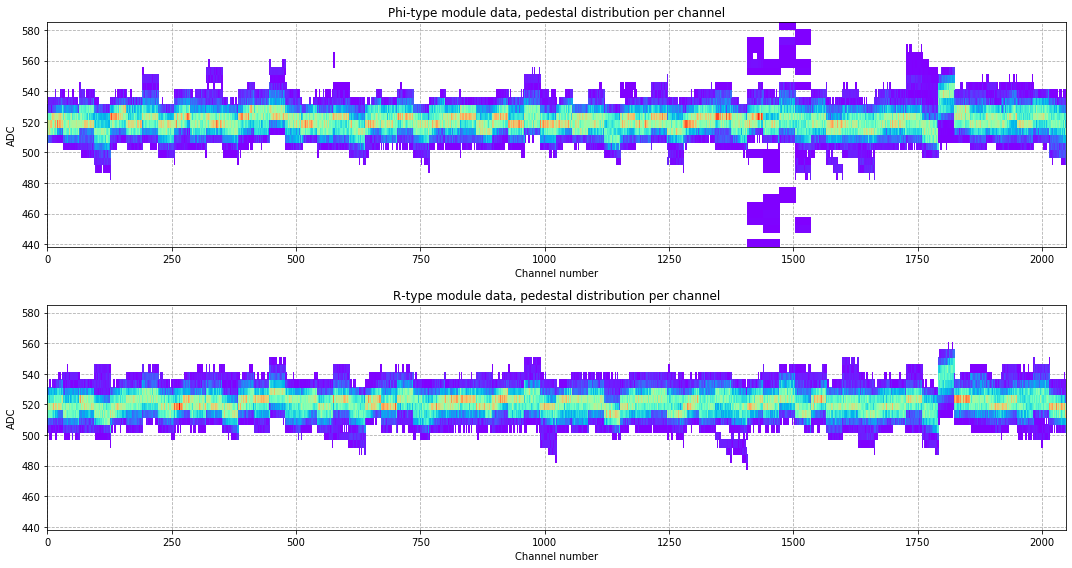
\includegraphics[width=0.5\linewidth]{figures/chapter4/calib_analysis/Part1-r-phi-pedestals.png}
    \caption{Histogram of the all of the pedestal values, across all of the calibrations The histogram above is $P_{Ch, R, \#, T}$ and the below $P_{Ch, \phi, \#, T}$).}
    \label{plot:part1-r-phi-pedestals}
\end{figure}


\begin{figure}
    \centering
    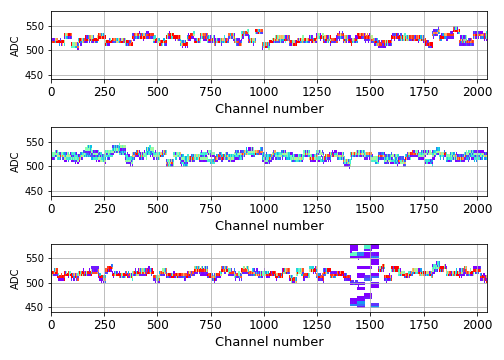
\includegraphics[width=0.5\linewidth]{figures/chapter4/calib_analysis/Part1-outliers-pedestals-cases.png}
    \caption{Pedestal plot for sensors $P_{Ch, R, \#64, T}$ $P_{Ch, R, \#35, T}$ $P_{Ch, R, \#85, T}$. $\#64$ and \#35 represent a typical pedestal values, while in \#85 there is a malfunction visible close to channel 1500.}
    %@TODO recast the sensors to their modules, and check the sensor type
    \label{plot:par1-pedestal-sensors}
\end{figure}

The radiation constantly damages the sensors, resulting in need of asjusting bias voltage
%@TODO make sure that you discuss what bias voltage is
The pedestals are actually a way of fine-tuning the levels of the signal. If the value of the pedestals would exhibit a trend this could mean that the bias voltage adjustment is not sufficient, or it doesn't give desired result. Thus, a study of the trend of the pedestals is important aspect of this analysis. The trend was calculated by fitting a line ($y=ax+b$) to the pedestal values in the time (calibration) domain. The value of the linear coefficient ($a$) which is responsible for the trend, is calculated individually for each of the channels of the detector. The distribution of this coefficient is visible in the Fig. \ref{plot:part1-pedestal-trend}. The mean value of the coefficient is $9.63e-05$ which is so close to zero that it can be assumed that there is no overall trend.
%@TODO check the dimensionality of the coefficient!!!

\begin{figure}
    \centering
    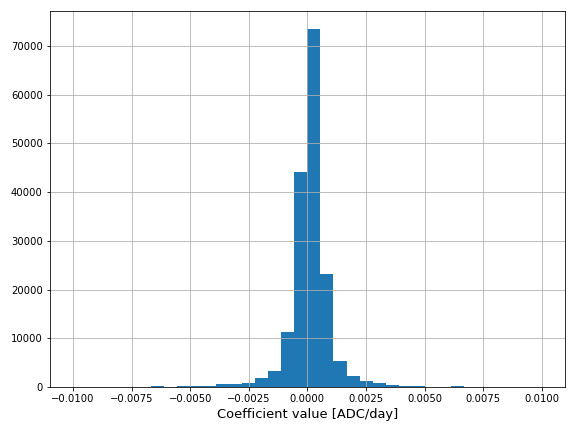
\includegraphics[width=0.7\linewidth]{figures/chapter4/calib_analysis/Part1-pedestal-trend.png}
    \caption{Histogram of linear coefficient of the pedestal trend per channel. Some of the outlyingcoefficient values have been trimmed,  and are outsidethe scope of this plot.}
    \label{plot:part1-pedestal-trend}
\end{figure}

\subsection{Threshold}

Of the two studied parameters, the high threshold parameter is the one actually responsible for the sensitivity of the detection of the hit. It is one of th many steps of filtering the signal coming from VELO. Further, the hit information is crutial for the reconstruction algorithms and particle detection and recognition. 
%@TODO maybe add a citation?
At first glance, a 2D histograms visible in Fig. \ref{plot:part2-threshold-all} is cluttered by outlying values. 
The most visible ones are near value 127 across all channels. This is actually an expected sight, as setting a value to 127 means the maximal possible value which makes the data coming from the channel unusable. This is a masking value, and occurances of those masks are discussed in detail in the next section. 
This comes from afaulty  sensor  \#67  and  dates  ’2016-11-07’  and  ’2016-11-11’,  where  the  threshold  value  reaches  400  ADC. This likely an error of that could accidentally get into the dataset, and yet there is no explanation for those values.
Moving on, we ignore those values, and limit the analysis to the range of values close to 0.

\begin{figure}
    \centering
    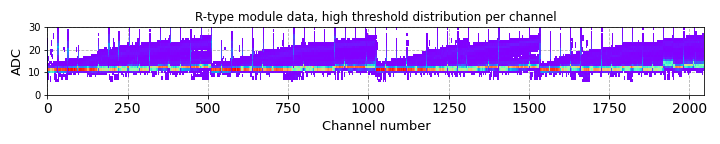
\includegraphics[width=0.7\linewidth]{figures/chapter4/calib_analysis/P2-threshold-all-zoom.png}
    \caption{High threshold distribution with header cross-talk. $H_t(Ch, \phi, \#, T)$ above and $H_t(Ch, R, \#, T)$ below.}
    \label{plot:P2-threshold-all-zoom}
\end{figure}

The Fig. \ref{plot:P2-threshold-all-zoom} depicts $H_t(Ch, R, \#, T)$ and $H_t(Ch, \phi, \#, T)$ in range of values from 0 to 30. One of the immidiatelly visible things are the vertical strips of low intensity, spaced throughout the channels. This a header cross-talk effect, in which the signal is disturbed.
% @TODO you will have to explaine the HC effect
In some cases it might be useful to exclude the channels that contain the header crosstalk effect, and the full list of the those channels is present in the appendix.
The $Ch*$ denotes all of the channels withouth the header cross-talk effect. 
% @TODO add the HC channel list and reference it here.
The reader can examine the difference of the histogram with and without header cross-talk in the Fig. \ref{plot:P2-threshold-all-zoom} and \ref{plot:P2-threshold-all-zoom-nohc}.

\begin{figure}
    \centering
    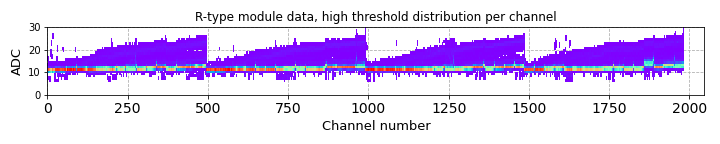
\includegraphics[width=0.7\linewidth]{figures/chapter4/calib_analysis/P2-threshold-all-zoom-nohc.png}
    \caption{High threshold distribution without header cross-talk. $H_t(Ch*, \phi, \#, T)$ above and $H_t(Ch*, R, \#, T)$ below.}
    \label{plot:P2-threshold-all-zoom-nohc}
\end{figure}


\begin{figure}
    \centering
    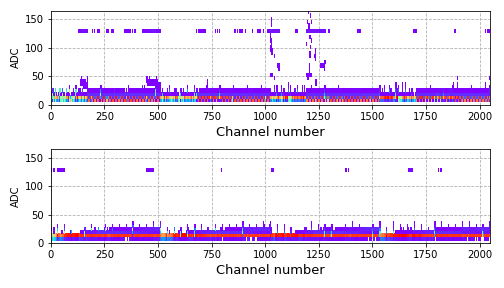
\includegraphics[width=0.7\linewidth]{figures/chapter4/calib_analysis/P2-threshold-all-r-phi.png}
    \caption{High threshold distribution of all of the calibrations, across all sensors. $H_t(Ch,\phi,\#, T)$ is above, and $H_t(Ch,\phi,\#, T)$ is the plot below.}
    \label{plot:part2-threshold-all}
\end{figure}

Another insight coming from the 2D histogram coming from the Fig. \ref{plot:P2-threshold-all-zoom-nohc} is that there are regularities of low intensity, repeating roughly every 512 channels. The periodicity of those regularities comes from the design of the sensors, and the pattern of the sitribution of that the channels and their lines.
(@TODO what lines)
More precisely they are recognised as imperfect calibrations coming from two dates  '2012-07-30', '2012-08-01'.
Those two dates are imperfect due to the power break occuring on those dates.
This imperfect calibration was influencing the sensitivity of the detector, and overall data taking.
Additionally for the purpose of outlierness analysis two calibration dates also being are recognised as imperfect 2012-08-02 and 2011-03-07.
Those occurances of the miscalibration are a direct motivation for detecting anomalies in the calibration in section \ref{chap4:outlierness}.


\begin{figure}
    \centering
    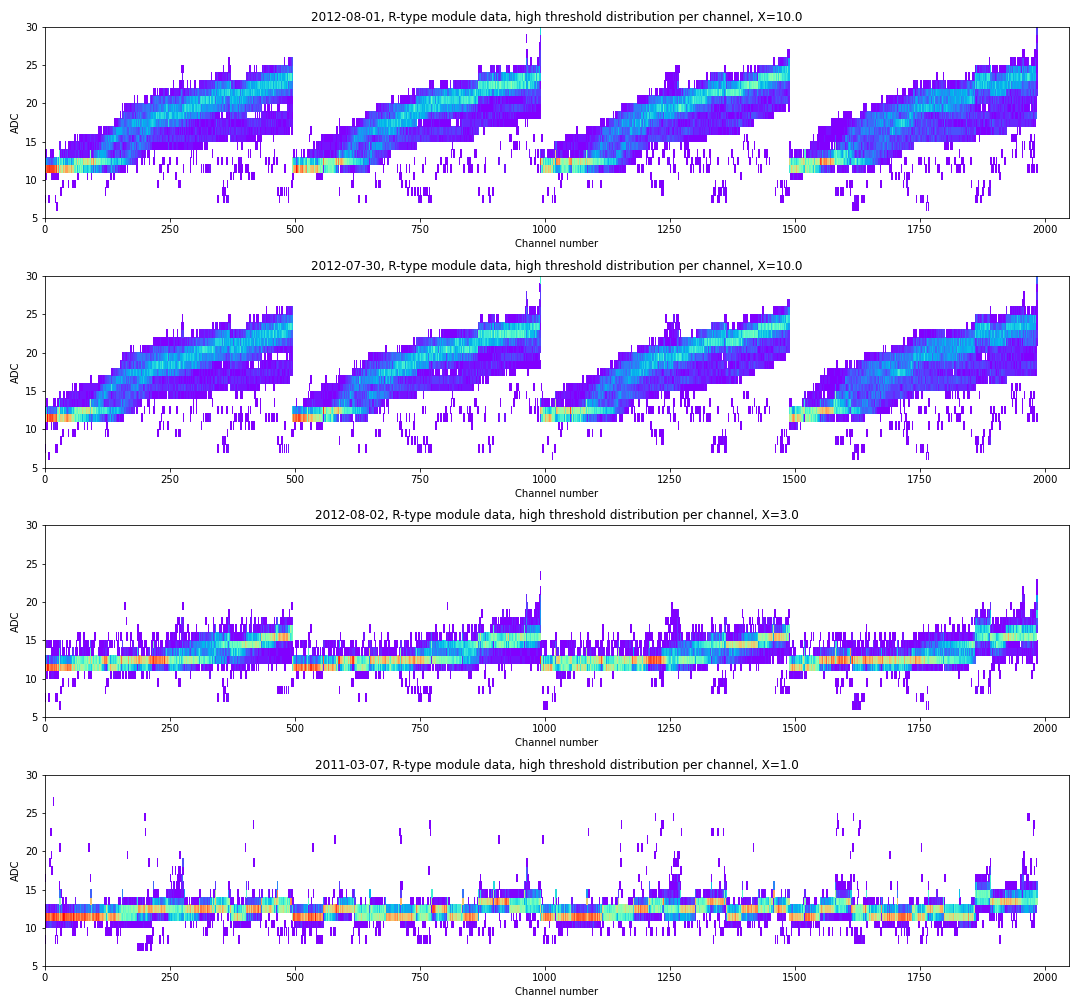
\includegraphics[width=0.6\linewidth]{figures/chapter4/calib_analysis/P2-all-bad-cals-R.png}
    \caption{Various R type calibration dates, with assigned value of outlierness.}
    \label{plot:all-bad-r}
\end{figure}

\begin{figure}
    \centering
    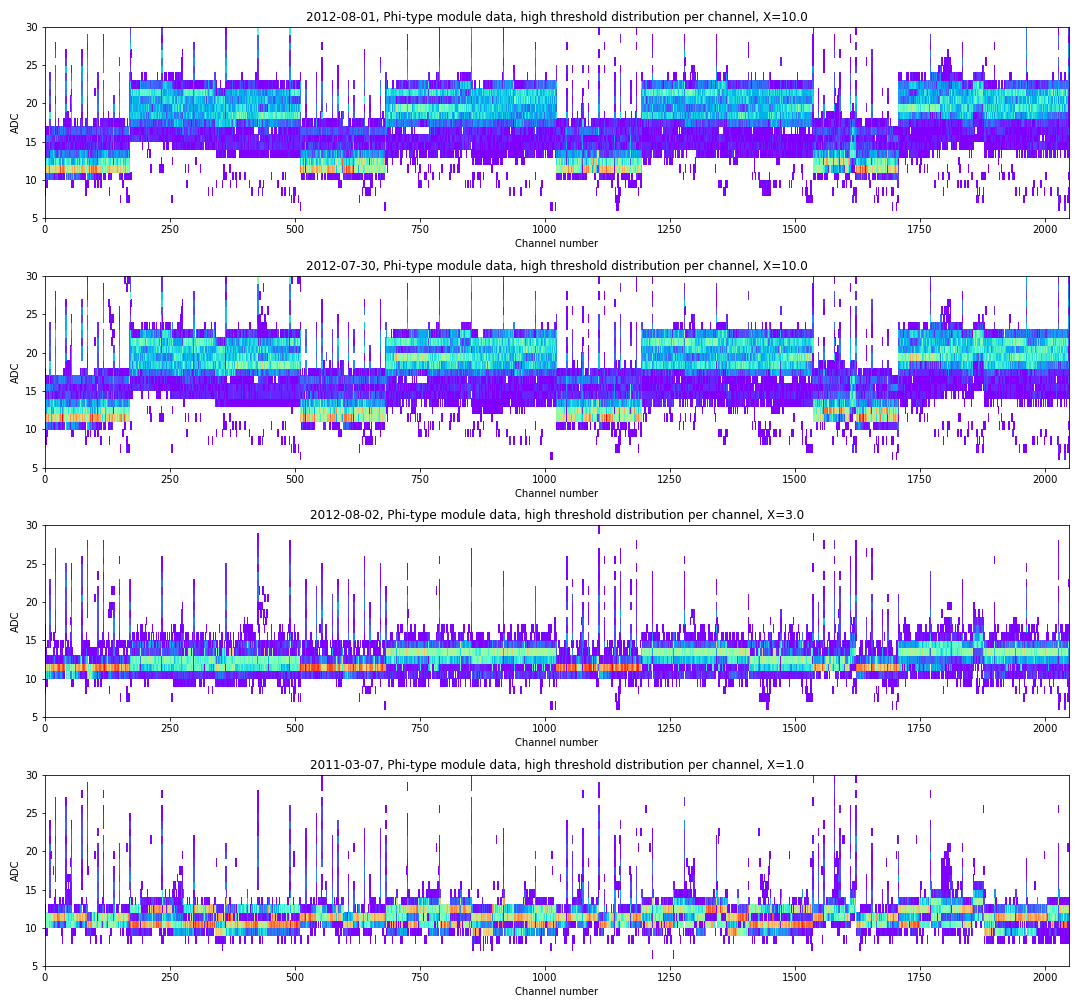
\includegraphics[width=0.6\linewidth]{figures/chapter4/calib_analysis/P2-all-bad-cals-phi.png}
     \caption{Various phi type calibration dates, with assigned value of outlierness.}
    \label{plot:all-bad-phi}
\end{figure}


\begin{figure}
    \centering
    
    \begin{subfigure}[b]{\textwidth}
    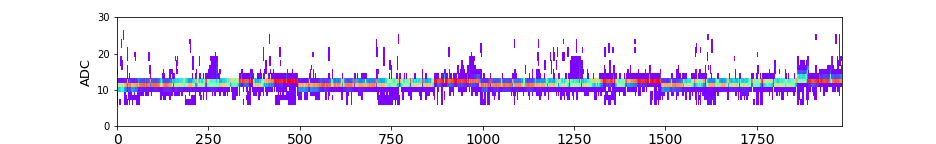
\includegraphics[width=\linewidth]{figures/chapter4/calib_analysis/P2-only-good-R.png}
    \caption{ .}
   \label{plot:only_good_r}
  \end{subfigure}
  
  \begin{subfigure}[b]{\textwidth}
    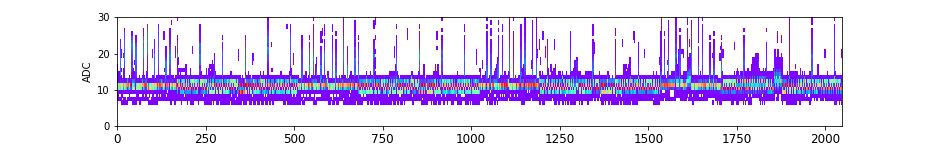
\includegraphics[width=\linewidth]{figures/chapter4/calib_analysis/P2-only-good-phi.png}
    \caption{ .}
   \label{plot:only_good_phi}
  \end{subfigure}
      \caption[All calond]{All of the calibrations, with reduced dimentionality using autoencoder and PCA.}
    \label{plot:only_good_all}
  
  \end{figure}



\subsection{Masked Values and others}



  As mentioned previously, the $H_t=127 ADC$ means that the channel is being masked.
  Setting the threshold so high, means that no hit will be registered in a given channel.
  The masks were given to the channels that exhibited exceptional noise levels.
  Their occurances are depicted in Figs \ref{plot:p3-mask-time} and \ref{plot:p3-mask-time2}.
  In  \ref{plot:p3-mask-time} the channels from all calibration are plotted as number of blocked channels per sensor in time domain.
  The important insight is that some sensors are more prone to masking channels than others, and that during the ammount of masked channels changes.
  In some cases the masked channels can go away and come back into the sensor.
  The figure \ref{plot:p3-mask-time2} depicts number of masked channels in time domain, with a sensor split.
  It is clearly visible that the total number of masked channels grows with time.
  (@TODO show that this goes in hand with total luminosity).
  This is expected as with time the negative radiation effects accumulate.

\begin{figure}
    \centering
    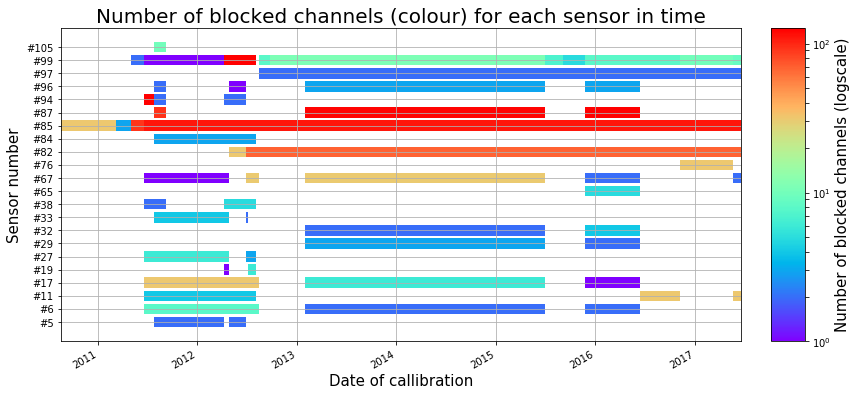
\includegraphics[width=0.7\linewidth]{figures/chapter4/calib_analysis/P3-mask-time.png}
    \caption{Distribution of blocked channels per sensor in time.}
    \label{plot:p3-mask-time}
\end{figure}

\begin{figure}
    \centering
    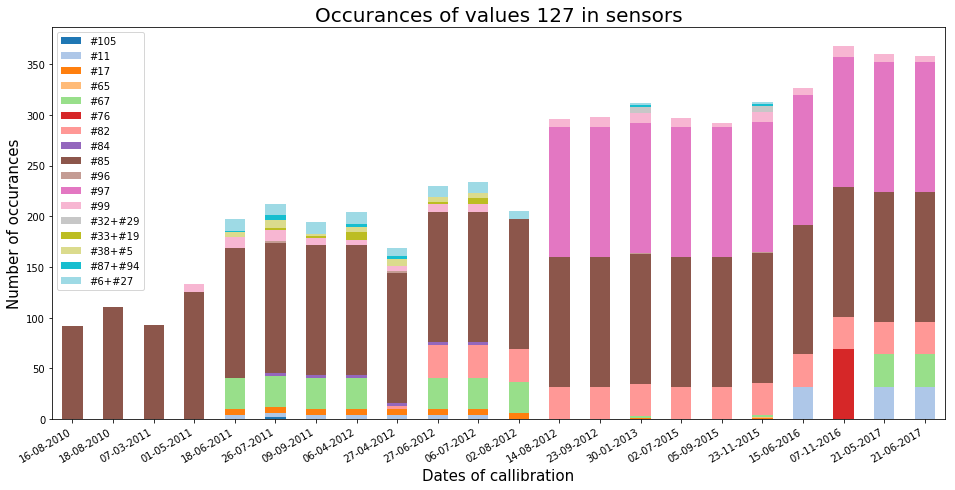
\includegraphics[width=0.7\linewidth]{figures/chapter4/calib_analysis/P3-mask-time2.png}
    \caption{Total number of occurances of masked channels versus time.}
    \label{plot:p3-mask-time2}
\end{figure}

Apart from the masked values, the usual and outlying calibration, there is still a part of the data which doesn't fit any of those categories.
This part of data can be characterised as the $H_{t} > 50 ADC \land H_{t} \neq 127 ADC$.
In the Fig \ref{plot:p3-other-outliers} depicts those other outliers. Number of occurances of these outliers change from calibration to calibration, but overall is limited to three sensors: \#85 \#67 and \#94.


\begin{figure}
    \centering
    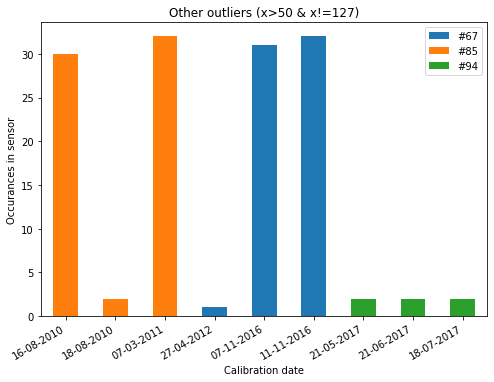
\includegraphics[width=0.7\linewidth]{figures/chapter4/calib_analysis/P3-other-outliers.png}
    \caption{Outlying values other than masked channels.}
    \label{plot:p3-other-outliers}
  \end{figure}

\section{Outlierness with probabilistic programming}
\label{chap4:outlierness}

\subsection{Dataset creation}
The analysis of the calibration data in the previous section yielded a usefule insight into the properties of the high threshold $H_t$.
A standard calibration for $R$ of $\phi$ sensor is usually close to certain value, independant of the calibration.
It is assumed that the distribution of the threshold value is given by the gaussian distribution.
The analysis of the bad (@TODO add asterisk here) calibrations shows that actually that the distribution $H_t$ is alaso dependant on the channel (e.g the regularity repeating every 500 channels).
The ``bad'' calibrations were assigned an ``outlierness'' value $X$.
This ``outlierness'' measure is purely artificial and subjectine, and also expresses a strenght of belief that a given calibration is an outlier.
The bigger the number, the stronger the belief that calibration is outlier.
There is no scale or limit on the outlierness number, other than that the 0 represents a normal calibration.
The actual assigned values can be seen in the Table \ref{data-table}.

\begin{table}[h]
\caption{\label{data-table}Outlierness calibration dataset values.}
\begin{center}
\begin{tabular}{ll}
Calibration date& X\\
2011-03-07&1\\
2012-08-02&3\\
2012-07-30&10\\
2012-08-01&10\\
all others&0\\
\end{tabular}
\end{center}
\end{table}

\subsection{Model}

For the purpose of simplicity this subsection, we will be using only the $R$-typed sensor data, and decribe a notation (@TODO linebreaks in the equation):


\begin{equation}
  \label{notation}
   T_n = H_{n}(n, R, \#, T*) \land T\prime_n = H_{n}(n, R, \#, T)
  \end{equation}

Where $n$ stands for a channel number across all sensors in time.
As mentioned previously, it is assumend that the distribution of the threshold in particular channel is gaussian.

\begin{equation}
  \label{basoc-model}
    T_n \sim Gaussian(\mu=\mu_n, \sigma=\sigma_n)
  \end{equation}

As visible in \ref{plot:only_good_all}, the value of the normal calibration for the $R $ sensor oscillates around $12 ADC$.
Therefore the parameters $\mu_{n}$ and $\sigma_{n}$ can be calculated by fitting the channels histogram to gaussian distribution.
In this case the probabilistic programming paradigm is used to achieve that. We use the dataset containing only ``good'' calibrations to calculate that.

In order to extend the model to the ``bad'' calibrations, we add additional terms to the model:

\begin{equation}
    \label{total-model}
    T\prime_n \sim Gaussian(\mu=X*\mu\prime_n+\mu_n, \sigma=X*\sigma\prime_n+\sigma_n)
\end{equation}

The $X$ stands for the outlierness of the calibration, and $\mu\prime$ and $\sigma\prime$ are coefficients of the linear dependency on the $X$.
These parameters, as previously are intrinsic property of $n$ channel.
The $X$ value is the same across given calibration date.
Notice that when the $X=0$, then, the model in Eq. \ref{total-model} is equivelent to \ref{basoc-model}.
This allows to use the parameters $\mu_{n}$ and $\sigma_{n}$ calculated for previous model, to be used in the extended one.
Given the $X$ from the \ref{data-table}, we are able to calculated $\mu\prime_{n}$ and $\sigma\prime_{n}$.

\subsection{Training}
(@TODO) add details about pymc training here

\subsection{Results}

The model presented in this subsection is a machine learning model, but is quite different from the models used frequently (such those based on neural networks).

It is not a black-box model, as for each of the channels there are only 4 parameters that are needed. Such low complexity of the model also allows for no train-test split (a usual practice in mahcine learning).
This approach has additional benefits such as:

\begin{itemize}
  \item Partial dimentional independence - This model can be used to extract the value of the outlierness not only for entire calibration, but also for a specific sensor, or module, or a group of channels, or even just specific channels. When analysing the calibration this allows for a more detailed insight as it can bring focus to a specific part of a detector that exhibits more unpredicted behaviour.
  \item Generation of artificial data - Because the probabilistic programing is based upon the statistical inference, and distributions, simply by calculating the $\mu$ and $\sigma$ parameters of gaussian distribution we are able to generate an artificial sample of the data.
  \item Interpolation and Extrapolation - This model was trained only on four different values of $X$, and yet, it is capable to asses the outlierness value not only in the range between those four values (e.g. $X=5$), but also through generation of artificial data, in can show what a calibration that this outside the scope of the data (e.g. $X=12$) might look like.
\end{itemize}

\begin{figure}
    \centering
    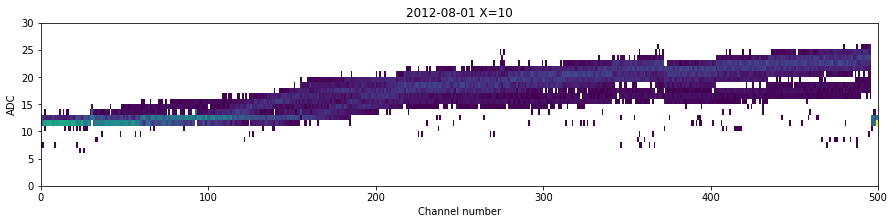
\includegraphics[width=0.7\linewidth]{figures/chapter4/outlierness/real_data.png}
    \caption{500 channels from a single calibration date marked with X=10}
    \label{plot:real-data}
  \end{figure}

\begin{figure}
    \centering
    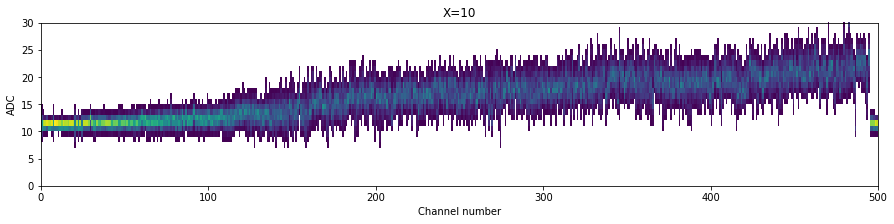
\includegraphics[width=0.7\linewidth]{figures/chapter4/outlierness/generated_data.png}
    \caption{500 channels from a single generated calibration at X=10}
    \label{plot:generated-data}
  \end{figure}

In Fig. \ref{plot:real-data} there is a sample of the data (500 chanels) that was taken of the ``bad calibrations''. It can be noted that the range of the $H_{t}$ values is on par with thos visible in the plot of the generated dataset \ref{plot:generated-data}.
(@TODO add another figure with artificial data of 12, and reference it here) Additionaly Fig there is a plot of calibration with value $X=12$, which was not present in the dataset and is actually outside the scope of the dataset.

This model was actually introduced to the Lovel monitoring system in the second half of year 2018, and was used to monitor the oncoming calibrations. The Figure \ref{plot:gui} depicts a screenshot from the monitoring system, and shows outlierness levels for the sensor \# 21. It is noticable that the value of the outlierness was slightly eleveted in 2017, which is attributed to some changes in the cooling system.


\begin{figure}
    \centering
    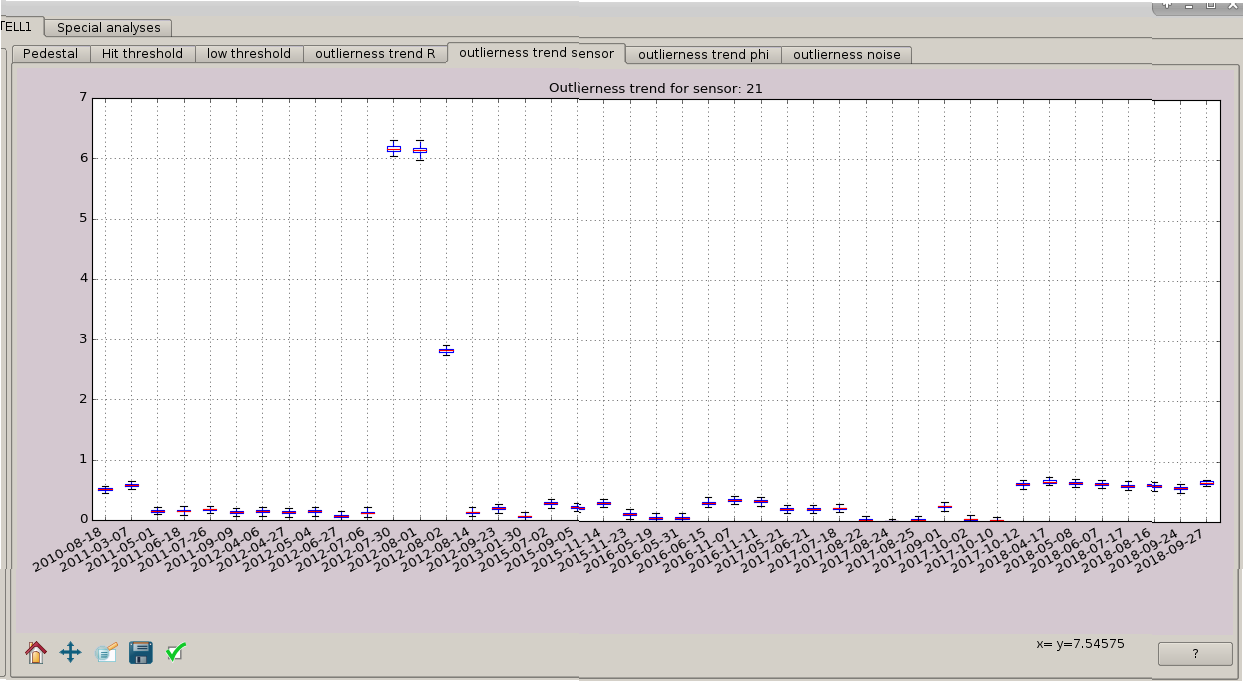
\includegraphics[width=0.7\linewidth]{figures/chapter4/outlierness/calina_lovell_screenshot.png}
    \caption{Screenshot from the outlierness monitoring in Lovell software.}
    \label{plot:gui}
  \end{figure}


\section{Dimentionality reduction}
\label{chap4:dimred}

The Velo detector in it's strip version, has 172 032 strips. Many of the parameters needed for it's calibration are calculated per strip. This is a huge amount of parameters, which is not easilly understable for human operators.
In it's pixel version, the number of such parameters will grow to 41 million (exactly $256*256*12*52 = 40894464$) \cite{Collaboration:1624070}.
Thus, an early tests of dimentionality reduction techniques will be very useful for the future. In this section we will only use high threshold parameter.
There are mutliple ways of applying PCA or autoencoder to the dataset (using different set's of values - or dimentions).
\subsection{Methods}

% @TODO explain why those two and not VAE or else
% @TODO reference the section
\subsection{Pedestals dimentionality reduction}

For the purpose of looking at what differentiates the pedestal parameter in some sensors frome the others. For this purpose we used PCA reduction, by reducing each channels time progression (a single dimentionality reduction for each of the sensor's channel).
The combined result is visible on Fig. \ref{plot:pca_pedestals_all}. Because of the high number of individual sensors, the split into several plots gives more clarity (Fig. \ref{plot:pca_all_ped}).

\begin{figure}[H]
    \centering
    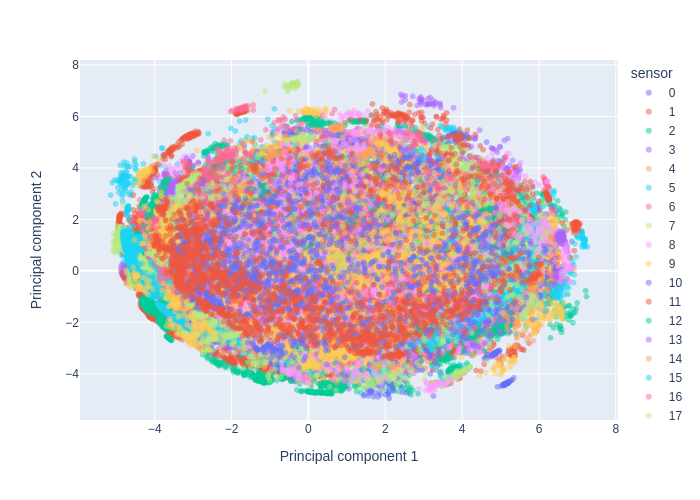
\includegraphics[width=0.7\linewidth]{figures/chapter4/dimred/PCA_pedestals_all.png}
    \caption{}
   \label{plot:pca_pedestals_all}
  \end{figure}

The reduced dataset shows a 2D gaussian distribution. It can be seen that some of the channels from a particular sensor can form clusters, or be distributed on a ring on the border of the dataset. What actually happens with a single datapoint with the tranformation can be explained by examining the particular channels. In the Fig. TODO there are 3 selected channels from a plot of the reduced data in sensor 11. Those points are also plotted at the Fig. TODO. We can see that the sensors on the opposing edges of the circle formed by the data, represent different trends in the pedestals value. Channel's 1899 pedestal value grows over time, but 543's decreases. Values in channel 322 stays high and stable. Therefore we can say that that essentially the PCA reduction separates the channels based on their trend. The 2D gaussian distribution structure makes it consistent with the trend calculation in previous sections, as the distribution centers around 0. This means that there is no overall trend (no growth, or decrease).
  
  \begin{figure}
\centering
\begin{subfigure}[b]{0.45\textwidth}
    \centering
    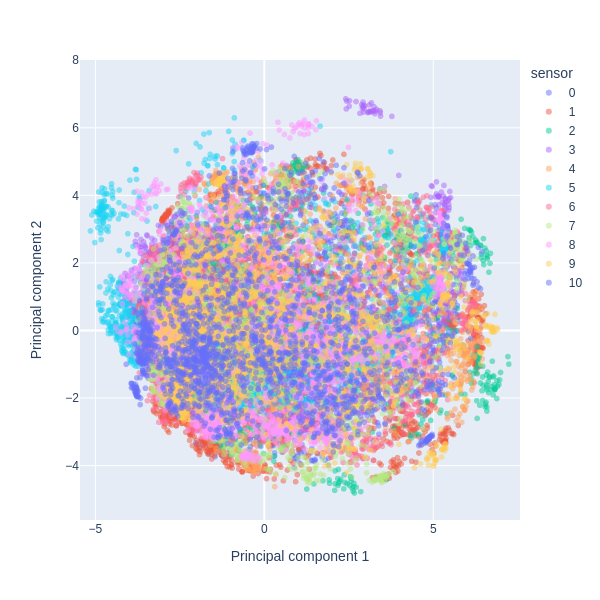
\includegraphics[width=\linewidth]{figures/chapter4/dimred/PCA_pedestals_r_phi_0.png}
\caption{PCA, R sensor type}
  \label{plot:PCA_pedestals_0}
  \end{subfigure}
\begin{subfigure}[b]{0.45\textwidth}
    \centering
    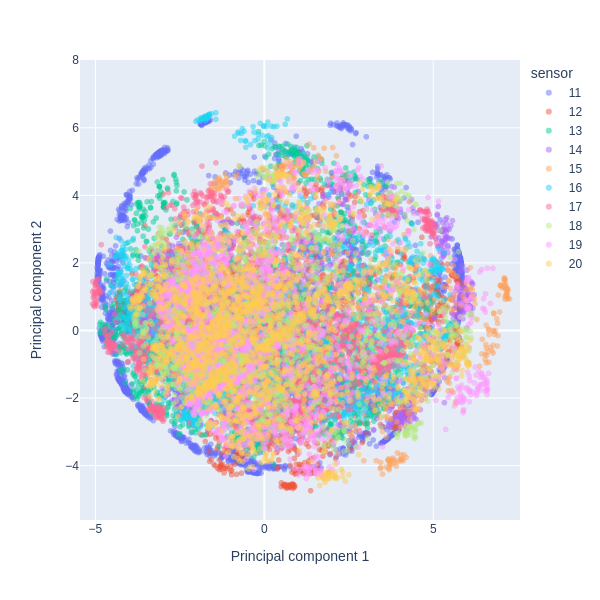
\includegraphics[width=\linewidth]{figures/chapter4/dimred/PCA_pedestals_r_phi_1.png}
\caption{PCA, phi sensor type}
   \label{plot:PCA_pedestals_1}
  \end{subfigure}


\begin{subfigure}[b]{0.45\textwidth}
    \centering
    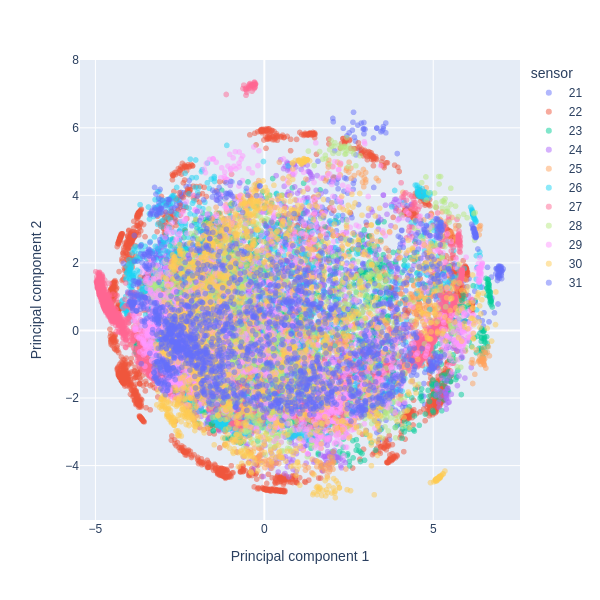
\includegraphics[width=\linewidth]{figures/chapter4/dimred/PCA_pedestals_r_phi_2.png}
% \caption{}
\caption{autoencoder, R sensor type}
    \label{plot:PCA_pedestals_2}
  \end{subfigure}
\begin{subfigure}[b]{0.45\textwidth}
    \centering
    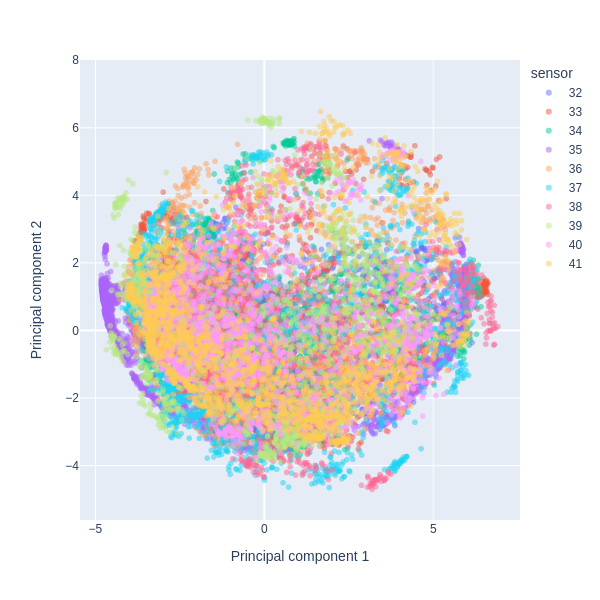
\includegraphics[width=\linewidth]{figures/chapter4/dimred/PCA_pedestals_r_phi_3.png}
\caption{autoencoder, phi sensor type}
% \caption{}
   \label{plot:PCA_pedestals_3}
  \end{subfigure}

    \caption[All calibrationd]{All of the calibrations, with reduced dimentionality using autoencoder and PCA.}
    \label{plot:pca_all_ped}
\end{figure}



 \begin{figure}
\centering
\begin{subfigure}[b]{0.45\textwidth}
    \centering
    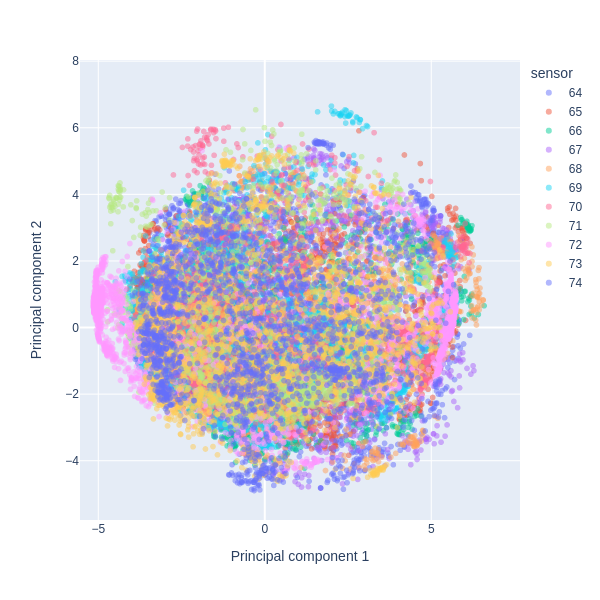
\includegraphics[width=\linewidth]{figures/chapter4/dimred/PCA_pedestals_phi_0.png}
\caption{PCA, R sensor type}
  \label{plot:PCA_pedestals_0_phi}
  \end{subfigure}
\begin{subfigure}[b]{0.45\textwidth}
    \centering
    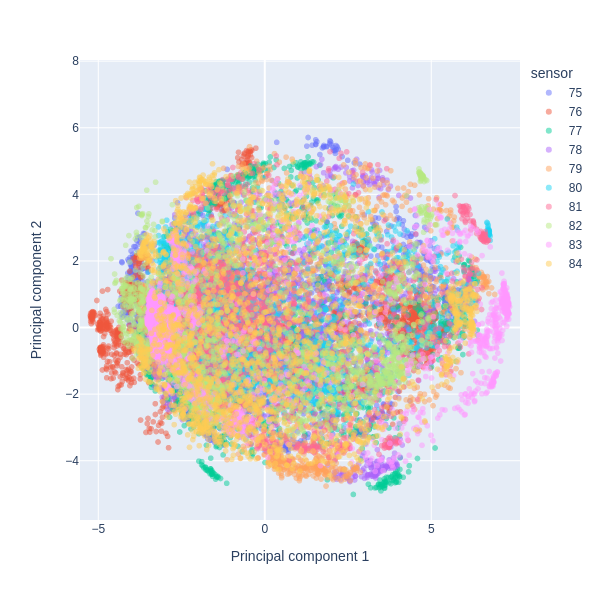
\includegraphics[width=\linewidth]{figures/chapter4/dimred/PCA_pedestals_phi_1.png}
\caption{PCA, phi sensor type}
   \label{plot:PCA_pedestals_1_phi}
  \end{subfigure}


\begin{subfigure}[b]{0.45\textwidth}
    \centering
    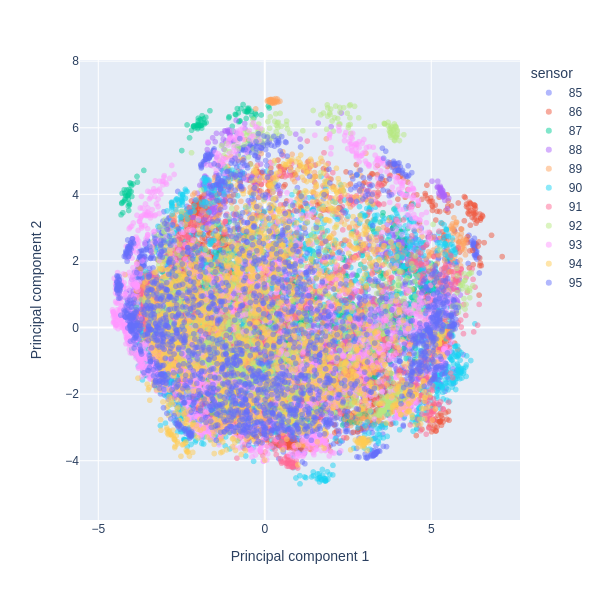
\includegraphics[width=\linewidth]{figures/chapter4/dimred/PCA_pedestals_phi_2.png}
% \caption{}
\caption{autoencoder, R sensor type}
    \label{plot:PCA_pedestals_2_phi}
  \end{subfigure}
\begin{subfigure}[b]{0.45\textwidth}
    \centering
    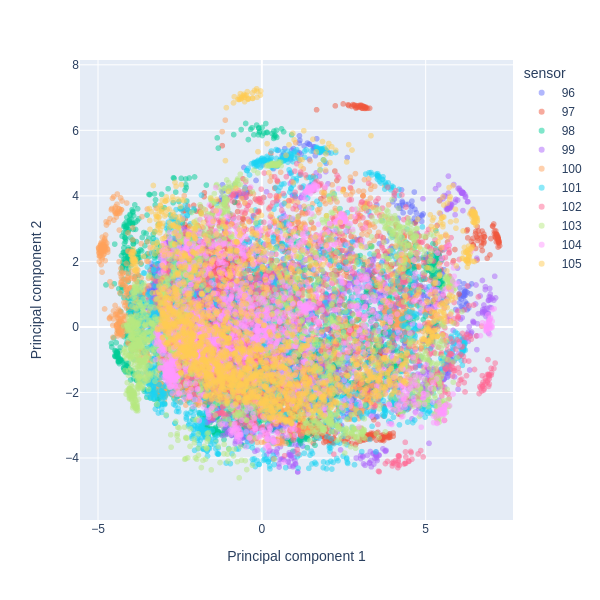
\includegraphics[width=\linewidth]{figures/chapter4/dimred/PCA_pedestals_phi_3.png}
\caption{autoencoder, phi sensor type}
% \caption{}
   \label{plot:PCA_pedestals_3_phi}
  \end{subfigure}

    \caption[All calibrationd]{All of the calibrations, with reduced dimentionality using autoencoder and PCA.}
    \label{plot:pca_all_ped_phi}
\end{figure}


\begin{figure}
    \centering
    
    \begin{subfigure}[b]{.5\textwidth}
    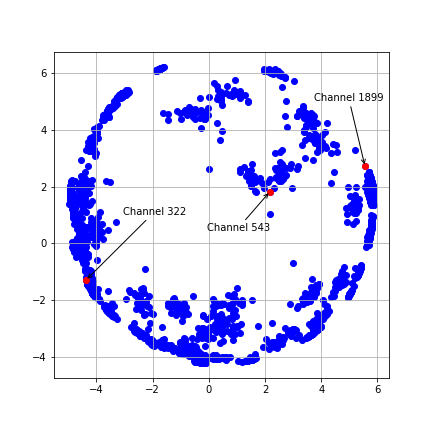
\includegraphics[width=\linewidth]{figures/chapter4/dimred/selected_channels_ped.png}
    \caption{ .}
   \label{plot:PCA_selected}
  \end{subfigure}\begin{subfigure}[b]{.5\textwidth}
    \includegraphics[width=\linewidth]{figures/chapter4/dimred/PCA_trends_channel.png}
    \caption{ .}
   \label{plot:PCA_trend}
  \end{subfigure}
      \caption[All calond]{All of the calibrations, with reduced dimentionality using autoencoder and PCA.}
    \label{plot:pca_all}
  
  \end{figure}





\subsection{Threshold dimentionality reduction}


The most usefult is feeding the algorithm with each of the sensors, with separation for the R and phi types of sensors.
This allows us to easilly see changes common for all of the sensor at once.
In Figures \ref{plot:pca_progression_r}-\ref{plot:nn_progression_phi}, you can see ten consecutive calibrations plotted after dimentionality reduction of a single sensor ($n_{dim}=2048$) to a 2D ($n_{dim}=2$), and plotted on a plane.
The color represents the number of a sensor.
In both of the plots made using PCA and autoencoders you can see that two outlying dates (2012-07-30 and 2012-08-01) stand out significantly.
In contrast with autoencoder, the PCA is deterministic, and does not require random initialisation. Because of this, there may be some variance in autoencoder model results, even when using exactly the same setup.

% \ref{plot:pca_progression_r},  \ref{plot:pca_progression_phi}, \ref{plot:nn_progression_r}, \ref{plot:nn_progression_phi},

\begin{figure}[H]
    \centering
    \includegraphics[width=\linewidth]{figures/chapter4/dimred/PCA_module_R_together.png}
    \caption{Time progression of selected section of calibration dates, with reduced dimentionality using PCA, only for R sensors.}
   \label{plot:pca_progression_phi}
  \end{figure}

\begin{figure}[H]
    \centering
    \includegraphics[width=\linewidth]{figures/chapter4/dimred/PCA_module_phi_together.png}
    \caption{Time progression of selected section of calibration dates, with reduced dimentionality using PCA, only for phi sensors.}
   \label{plot:pca_progression_r}
  \end{figure}

\begin{figure}[H]
    \centering
    \includegraphics[width=\linewidth]{figures/chapter4/dimred/NN_module_R_together.png}
    \caption{Time progression of selected section of calibration dates, with reduced dimentionality using autoencoder, only for R sensors.}
   \label{plot:nn_progression_r}
  \end{figure}

\begin{figure}[H]
    \centering
    \includegraphics[width=\linewidth]{figures/chapter4/dimred/NN_module_phi_together.png}
    \caption{Time progression of selected section of calibration dates, with reduced dimentionality using autoencoder, only for phi sensors.}
   \label{plot:nn_progression_phi}
  \end{figure}

  The Figures \ref{plot:pca_all_r}-\ref{plot:nn_all_phi} represent all calibration dates on the same plot, splitted into different sensors, and created with different techniques. Notice that all of the plots have different scales of the axes, as the methods used to reduce dimentionality do not retain the scale. The most useful insight to those plots is that the relative change represents outlying calibrations.

\begin{figure}
\centering
\begin{subfigure}[b]{0.45\textwidth}
    \centering
    \includegraphics[width=\linewidth]{figures/chapter4/dimred/PCA_module_R_all.png}
\caption{PCA, R sensor type}
   \label{plot:pca_all_r}
  \end{subfigure}
\begin{subfigure}[b]{0.45\textwidth}
    \centering
    \includegraphics[width=\linewidth]{figures/chapter4/dimred/PCA_module_phi_all.png}
\caption{PCA, phi sensor type}
   \label{plot:pca_all_phi}
  \end{subfigure}


\begin{subfigure}[b]{0.45\textwidth}
    \centering
    \includegraphics[width=\linewidth]{figures/chapter4/dimred/NN_module_R_all.png}
% \caption{}
\caption{autoencoder, R sensor type}
   \label{plot:nn_all_r}
  \end{subfigure}
\begin{subfigure}[b]{0.45\textwidth}
    \centering
    \includegraphics[width=\linewidth]{figures/chapter4/dimred/NN_module_phi_all.png}
\caption{autoencoder, phi sensor type}
% \caption{}
   \label{plot:nn_all_phi}
  \end{subfigure}

    \caption[All calibrationd]{All of the calibrations, with reduced dimentionality using autoencoder and PCA.}
\end{figure}
\section{Time to calibration forecasting}
\label{chap4:wtte}
The calibration of the detector is essential for it's proper use. It set's all of the parameters of the detector that will be needed during the data taking.
In Velo runs 1 and 2 of the LHC it was possible that if the channel thresholds were set too high, useful data could be lost. When a electrical signal coming from a single strip would not exceed the threshold, it would be discarded.
Therefore it is crutial for the detector operations to have as frequent calibrations as possible.
But the calibration process requires a noise data recorded when there is no beam present. Ideally, the longer the time that it takes to record the noise, the better the callibration accuracy (gaussian noise mean calculation. This also means that calibration requires a special time slot in between data taking, when no beam is present.
This motivates the studies of the forecasting of the need for calibration in Velo.

\section{Dataset}
In the data availible to the analysis we can distinguish two kinds of data: raw data and calibration data.
The raw data is the data that is recorded during the beam conditions, and the calibration data is the data taken during no-beam.
The actual way of calculating the values present in the data does not differ.
%@TODO reference the data analysis
\begin{figure}
    \centering
    \includegraphics[width=0.6\linewidth]{figures/chapter4/wtte/runlengths.png}
    \caption{Histogram of lengths of runs in the dataset, expressed in seconds. Significant ammount of runs lasted about 3600 seconds (1 hour).}
    \label{plot:runlen}
  \end{figure}
The ammount of datapoints is significantly greater for the raw data, as it was taken in any single data run, which can last from a few seconds, to about an hour.
Calibration data on the other hand was taken every few weeks.
In both kinds of the data there is a constant dimentionality of the parameters, as each of the values was taken for each of the 2048 channels of the sensor individually, in total giving a 172 032 values of a single parameter for the whole detector.
The analysis of the trends of the trends has produced a candidate for a parameter that could be used to identify a need for a calibration.
The \textit{pedestal subtracted} $\Delta\mu$  parameter is the value of the mean of the noise calculated as follows:
\begin{equation}
    \Delta\mu = \mu_{current} - \mu_{calibration}
\end{equation}
Where $\mu_{current}$ is mean of the signal coming from the current run.
The analysis of this parameter has shown that a value of the standard distribution of this paremeter $\sigma(\Delta\mu)$ within the detector grows after the calibration, and drops after one.
An example of this is present at the \ref{plot:wtte1-stdevs}.
\begin{figure}
\centering
\begin{subfigure}[b]{0.85\textwidth}
    \centering
    \includegraphics[width=\linewidth]{figures/chapter4/wtte/stdevs_trends_calibs.png}
% \caption{}
    \label{plot:wtte1-stdevs}
  \end{subfigure}

\begin{subfigure}[b]{0.85\textwidth}
    \centering
    \includegraphics[width=\linewidth]{figures/chapter4/wtte/pstdevs_trends_calibs.png}
% \caption{}
    \label{plot:wtte1-p-stdevs}
  \end{subfigure}

\begin{subfigure}[b]{0.85\textwidth}
    \centering
    \includegraphics[width=\linewidth]{figures/chapter4/wtte/rstdevs_trends_calibs.png}
% \caption{}
    \label{plot:wtte1-r-stdevs}
  \end{subfigure}
  \caption[Two numerical solutions]{ Standard deviation of the pedestal subtracted parameters in the whole sensor (top), pedestal subtracted in Phi sensors (middle), and in R sensors (bottom).
  Calibration dates are in red, and the green lines present trends calculated between calibrations.}
\end{figure}

% @TODO add image reference.

The data used for the forecasting model comes from 2018. The calibration process and raw data in 2018 is a best candidate because of the frequently occuring runs, and calibrations. The exact timespan of the data is from 2018-05-08 to 2018-09-24.
This constitues exactly 4 calibration periods. The used data comes in a form of $\sigma(\Delta\mu)_{t}$ where $t$ stands for a given run time.
The time information is translated to delta time ($dt_{n} = t_{n}-t_{n-1}$). The continious time series of data is processed to a windowed time-series, of 100 data points, beginning with the first data point after calibration, and padded with zeroes.

% @TODO show an examplary data
%

\begin{equation}
X_{it} = \begin{bmatrix} std_{it} \\ dt_{t} \end{bmatrix}
\end{equation}

As it is a case of supervised learning, the additional component $Y_{it}$ is set to be a number of days left until next calibration. We have chosen the number of days as the most suitable time range for this purpose, as there can be many runs per day,

% @TODO why not an exact time ?

\section{WTTE-RNN for Velo}


% @TODO reference the discussion of wtte-rnn
% @TODO explain why wtte-rnn

The WTTE-RNN as discussed in Sec ... is a one layer capable of outputing the parameters of the weibull distribution. The actual type of a problem in machine learning is called survival analysis, architecture of the neural network used for forecasting is present at the Table \ref{tab:network}. It contains 6 layers in total. The LSTM layer is necessary for the time series that is used as input data.

\begin{table}[h]
% https://app.neptune.ai/mmajewsk/wtte-calib/e/WTTEC-83/source-code?path=source_code&file=dense_module.py&attribute=files&filePath=.
\begin{center}
\begin{tabular}{ |c|c|c| }
\hline
Layer No. & Layer type & Layer size\\
\hline
1 & Dense & 43\\
2 & Dropout & \\
3 & LSTM & 20\\
4 & Activation - Tanh & \\
5 & Dense & 2\\
6 & WTTE-Activation & \\
\hline
\end{tabular}
\caption{\label{tab:network}The neural network layers used for the WTTE-RNN model}
\end{center}
\end{table}



\section{Mask clustering}

The VeloPix masks flags are veru useful things. They help to spot if there is something wrong with the detector.
%@TODO explain here where does the masks come from 
%@TODO explain here how come there are clusters in masks

The cluster masks can pose a threat to the reconstruction algorithm, and the radial reconstruction resolution.
As such they have to be monitored. 
\subsection{Mask simulation}

Due to the VeloPix being still under developement and comissioning during these studies, the experience gained with the tests of VeloPix was used to create a simulation of occuring masks.

%@TODO insert mask picture here

In order to make a realistic simulation we have used a process consisting of three types of intrusions:

\begin{itemize}
  \item Random uniform changes $P$, in which a random portion of pixels changes their state to masked
  \item Linear cluster $L$ where a linear portion of pixels are masked.
  \item Blob cluster $G$ with masks created by a 2D isotropic gaussian distribution.
\end{itemize}

These intrusions are added to an initially empty matrix with a different probabilities. Each of the intrusions is created on a empty matrix with the same size as the sensor, and is simply added to the simulated matrix $M$.
One crutial step of this simulation is random cleaning of the matrix, in which random 80\% of the pixels are unset to a non-mask state.
The pseudocode can be found in listing \ref{alg:two}.
This process creates a continious simulation of a VeloPix matrix masks, as the new masks and clusters are generated, and the old ones slowly dissappear.


%@TODO images !!!

\SetKwComment{Comment}{/* }{ */}

\begin{algorithm}[H]
\caption{An algorithm with caption}\label{alg:two}
\KwData{$n \geq 0$}
\KwResult{$y = x^n$}
$N \gets n$\;
\While{$N \neq 0$}{
  \uIf{random() $< blob\_prob $ }{
    $M \gets M + G$
  }
  \uElseIf{random() $< line\_prob $ }{
    $M \gets M + L$
  }
    \Else{$M \gets M + P$}
    $M \gets M + Pu$
    
    $N \gets N - 1$
}
\end{algorithm}




\subsection{Clustering}

There are many clustering algorithms present in the field of machine learning. Although they all come under the term "clustering" there are actually multiple different goals that can be achieved by different algorithms. The most common density search clustering algorithms are DBSCAN and OPTICS. The details of these algorithms are described in section \ref{sec:clustering}.
In the case of application of the clustering algorithm towards masks in calibration, the desired algorithm should be able to
%@TODO mention that clustering in this case does not mean to cluster all of the point on te matrix

\begin{figure}[h]
\centering
\includegraphics[width=0.5\textwidth]{figures/chapter4/velopix_clusters/dbscan_clusters.png}
\caption{And examplary clusterisation using DBSCAN ($\epsilon$ = 10, MinPts = 4) on the binary pixel-map. Clusters are numbered 1-5.}
\label{fig:dbscan_clusters}
\end{figure}

\subsection{Cluster features}

After finding the individual clusters on one calibration (a one set of masks), the clusters of masks can be characterised by a set of features.
\begin{enumerate}
\item \textbf{Position}  {$p_k$ = ($\bar{x_k}$, $\bar{y_k}$}), where $\bar{x_k} = \frac{\sum_{i}^{N^k}x_k^i}{N_k},
    \bar{y_k} = \frac{\sum_{i}^{N^k}y_k^i}{N_k}$.
\item \textbf{Size} $s_k$ = \{$n_k$, $d_k$\} where $n_k$ is the number of pixels in a cluster divided by the mean number of the pixels in the given sensor's clusters.
\item \textbf{Shape} $h_k$ = \{$\alpha_k$, $c_k$\}, where $\alpha_k$ is the directional coefficient of the cluster measured by the fit to the line $y^k(x) = \alpha_k*x + b_k$. The $c_k$ is the roundness of the cluster calculated as it's Pearson Coefficient.
\end{enumerate}
With those metrics, we can then define the spacial charecteristic vector as $v_k = [s_k; h_k]$. Then we define cluster as a set of unique features $cluster_k = {p_k, v_k}$.

\subsection{Cluster tracking}

This set of unique features is used to characterise every cluster found in the calibration.
The $cluster_{k}$ features are then used to identify cluster $k$ from timestep $t_{n}$ as te same in the timestep $t_{n-1}$.
It is performed by calculating a cosine similarity matrix $M$. The $M$ matrix is calculated in the following manner:

\begin{equation}
    M_{i,j} = \Phi_{i,j} * V_{i,j}
\end{equation}

Where $\Phi$ is defined as:
\begin{equation}
    \Phi_{i,j} = \frac{1}{d_{min}}*\max(d_{min} - D_{i,j}, 0)
\end{equation}

and $ D_{i,j} $ is a distance matrix:
 \begin{equation}D_{i,j} = || p_j - p_i ||\end{equation}

The value $d_{min}$ is set to be a limiting factor. If the distance of centroids of the clusters stays the same, the value is 1., but as the distance approaches $d_{min}$ the value approaches 0.
In the tests of the cluster tracking $d_{min}=10$ was used.
Exemplary pairing of the clusters in consecutive simulation steps is visible in the Fig. \ref{fig:fin_clus} with it's simmilarity matrix calculation in \ref{fig:sims}.

\begin{figure}[h]
\centering
\includegraphics[width=0.3\textwidth]{figures/chapter4/velopix_clusters/shape.png}
\includegraphics[width=0.3\textwidth]{figures/chapter4/velopix_clusters/distance.png}
\includegraphics[width=0.3\textwidth]{figures/chapter4/velopix_clusters/similarity.png}
\caption{Rows represent clusters on image A in Figure ~\ref{fig:fin_clus}, columns represent clusters on image B in Figure ~\ref{fig:fin_clus}. Values indicate the Spacial Characteristics Similarity Measure \textit{V} (left plot), and Positional Similarity Measure \textit{$\Phi$} (middle plot). The M matrix is the rightmost plot.
}
\label{fig:sims}
\end{figure}



\begin{figure}[H]
\centering
\includegraphics[width=0.7\textwidth]{figures/chapter4/velopix_clusters/paired.png}
\caption{Clusters labelled with the same integer are chosen by the algorithm as the consecutive generations of the same cluster. Clusters labeled as 'new' are clusters on the time step $t_{n}$ that were absent on time step $t_{n-1}$.}
\label{fig:fin_clus}
\end{figure}

 \subsection{Results}


The DBSCAN and OPTICS algorithms were tested on the 3000 consecutive steps of simulation of a single sensor.
The ground truth in context of clustering of the masks is not something that can v determined in the real world data.
But the simulation along with the simulation steps, can attribute any generated mask pixel to it's source (random uniform, linear, gaussian blob), thus providing information that can be used as ground truth.
It is assumed that the generated pixel should be identified as belonging to a cluster after up to 8 timesteps.
The Table \ref{sample-table} presents a confusion matrix calculated using that ground truth information. The OPTICS algorithm has three more times as many false positives as the DBSCAN. On the other hand it has almost twice more true positives.


\begin{table}[H]
  \caption{Confusion matrix values in 3000 consecutive simulation steps.}
  \label{sample-table}
  \centering
  \begin{tabular}{lll}


    \toprule
    Value     & OPTICS     & DBSCAN \\
    \midrule
    True Negative & 7608 & 16207 \\
    False Positive    & 11680 & 3081      \\
    False Negative     & 1156       & 3167  \\
    True Positive &  5665 &   3654   \\
    \midrule
    Accuracy &  0.51 &   0.76   \\
    Precision &  0.33 &   0.54   \\
    \bottomrule

  \end{tabular}
\end{table}

Both algorithms have been tested towards the ability to track the consecutive cluster's pixels through the steps of the simulation. Fig. \ref{fig:decay} depicts the number of the masks assosiated with any cluster starting at the timestep of introduction of said masked pixel. It is clearly visible that The OPTICS algorithm recognises more pixels as belonging to clusters, and for extended ammount of time, whereas the DBSCAN very quickly drops it's attention to the pixels.

\begin{figure}[H]
\centering
\includegraphics[width=0.4\textwidth]{figures/chapter4/velopix_clusters/optics_decay.png}
\includegraphics[width=0.4\textwidth]{figures/chapter4/velopix_clusters/dbscan_decay.png}
\caption{The fraction of pixels categorised as belonging to any clusters (Y axis) in next consecutive calibrations (X axis), since the cluster introduction to calibration (number of timesteps $n=300$). The number of detected pixels slowly decreases with time. The OPTICS algorithm (left plot) recognises the pixels of the clusters as belonging to a cluster (not necessarily the same one) for a longer amount of time. The DBSCAN is more strict in distinguishing the pixels that belong to clusters.
}
\label{fig:decay}
\end{figure}

The important test is the influence of the clustering algorithm towards the cluster tracking ability. The Fig. \ref{fig:progress} shows total number of clusters in given timestep of a simulation, being recognised as new, or retaining from previous timestep. It is clear that the cluster tracking with OPTICS detects much more clusters as new, and looses more clusters from callibration to callibration, whereas the DBSCAN, if finding less new clusters, and retaining old ones.

\begin{figure}[H]
\centering
\includegraphics[width=0.4\textwidth]{figures/chapter4/velopix_clusters/optics_progress.png}
\includegraphics[width=0.4\textwidth]{figures/chapter4/velopix_clusters/dbscan_progress.png}
\caption{ The number of clusters classified as being "old" - same as in previous calibration (blue colour), and a number of clusters marked as "new" - not being the same clusters as in previous calibration (orange color). The left plot belongs to OPTICS, and the one on the right to DBSCAN.
}
\label{fig:progress}
\end{figure}

\section{Studies of surrogate function in VeloPix}

(@TODO add something here)
\subsection{Surrogate function}

(@TODO add something about how the surrogate functions works, that there is somne charge created at the sensors to calibrate)
The surrogate function is the function that relates the TOT count to the charge gathered in the VeloPix pixel \cite{Tsopelas:2016cjb}.
It has the following structur:

% \begin{equation}
%   \label{eq:surrogate}
%   ToT(q) = g \dot q + ToT_{0} - \frac{c}{q-t} + o
%   \end{equation}


\begin{equation}
  \label{eq:surrogate}
  ToT(q) = p_{0} + p_{1} \dot q - \frac{c}{q-t}
  \end{equation}
It has four free parameters: $p_{0},p_{1},c,t$, and is essentially a convolution of linear and hyperbolic functions. There is existings underlying assumption that $q > 0$.
An examplary surrogate function is visible on \ref{fig:surrogate} (@TODO explain that plot better)


\begin{figure}[H]
\centering
\includegraphics[width=0.7\textwidth]{figures/chapter4/surrogates/surrogate_example.png}
\caption{An examplary plot of surrogate funciton.}
\label{fig:surrogate}
\end{figure}

\subsection{Dataset}

This analysis uses the dataset gathered during the testbeam phase of the Velopix.
(@TODO explaine the testbeam here)
(@TODO explain the sensor markings here)

\subsection{Cross sensor study}
The test beam data contained multiple different types of sensors, with different types of irradiation.
Unfortunately, in the entire datsaet, there is only one sensor that is suitable for the studies of surrogates in function of fluence.
This is due to the irradiation profile of the sensors. Sensor s8 was the only one that had a clear, non-uniform profile of the irradiation, that allowed for a binning of the sensor based on the ammount of irradiation that the sensors were exposed to.

nonetheless we investigate other sensors and their distribution of the parameters in the Fig. \ref{fig:sensor_surrogate_p1}  and \ref{fig:sensor_surrogate_p2}.
The important insight is that for most of the sensors, the overall distribution post irradiation moved to the left for the $p0$ and $p1$.
For the parameters $c$ and $t$ the trend is not as obvious, and we will explain the further analysis.


\begin{figure}
\centering
\begin{subfigure}[H]{0.85\textwidth}
    \centering
    \includegraphics[width=\linewidth]{figures/chapter4/surrogates/p1_S8_histos.png}
% \caption{}
    % \label{plot:wtte1-stdevs}
  \end{subfigure}

\begin{subfigure}[b]{0.85\textwidth}
    \centering
    \includegraphics[width=\linewidth]{figures/chapter4/surrogates/p1_S16_histos.png}
% \caption{}
    % \label{plot:wtte1-stdevs}
  \end{subfigure}

\begin{subfigure}[b]{0.85\textwidth}
    \centering
    \includegraphics[width=\linewidth]{figures/chapter4/surrogates/p1_S17_histos.png}
% \caption{}
    % \label{plot:wtte1-stdevs}
  \end{subfigure}

\begin{subfigure}[b]{0.85\textwidth}
    \centering
    \includegraphics[width=\linewidth]{figures/chapter4/surrogates/p1_S21_histos.png}
% \caption{}
    % \label{plot:wtte1-stdevs}
  \end{subfigure}

\begin{subfigure}[b]{0.85\textwidth}
    \centering
    \includegraphics[width=\linewidth]{figures/chapter4/surrogates/p1_S22_histos.png}
% \caption{}
    % \label{plot:wtte1-stdevs}
  \end{subfigure}

\label{plot:sensor_surrogate_p1}
  \caption[Surrogate parameters distribution part 2]{Part 1 of the distribution of the surrogates parameters in sensors. The rows of plot represent sensors, each of the columns of the plots reperesent a parameter of the surrogate (p0, p1, c, t).  The color blue (pre) denotes the distribution before irradiation of a given parameter, the orange color is the distribution after the irradiation of the sensor. }
\end{figure}

\begin{figure}[H]
\centering

\begin{subfigure}[b]{0.85\textwidth}
    \centering
    \includegraphics[width=\linewidth]{figures/chapter4/surrogates/p1_S27_histos.png}
% \caption{}
    % \label{plot:wtte1-stdevs}
  \end{subfigure}

\begin{subfigure}[b]{0.85\textwidth}
    \centering
    \includegraphics[width=\linewidth]{figures/chapter4/surrogates/p1_S29_histos.png}
% \caption{}
    % \label{plot:wtte1-stdevs}
  \end{subfigure}

\begin{subfigure}[b]{0.85\textwidth}
    \centering
    \includegraphics[width=\linewidth]{figures/chapter4/surrogates/p1_S30_histos.png}
% \caption{}
    % \label{plot:wtte1-stdevs}
  \end{subfigure}

\label{plot:sensor_surrogate_p2}
  \caption[Surrogate parameters distribution part2]{Part 2 of the distributions of surrogates parameters.}
\end{figure}


\subsection{The fluence}

As mentioned previously, the sensor S8 (@TODO maybe use different name here), was the only one that had a well documented non-uniform irradiation.
The irradiation profile is visible in the plot (@TODO) add the actual irradiation plot here.
For the purpose of this irradiation profile, we devise a binning visible in the Figure \ref{fig:binning}.
This binning allows for assigning values of fluence per each bin and analysis of the pixels groups in the binnning.
The fluence per bin is as seen in the table \ref{tab:fluence_per_bin}, the innermost bin has the highest fluence level.
This mean that we expect that the effects of the radiation will be most visible in the center of the pixel matrix.



\begin{figure}[H]
\centering
\includegraphics[width=0.7\textwidth]{figures/chapter4/surrogates/p2_binning.png}
\caption{A heatmap of the binning used in the analysis of the fluence. Each color represents a different elliptical binning. The binning starts from 0 in the center, and the outermost bin is labeled as 7.}
\label{fig:binning}
\end{figure}

(@TODO this tab, is mean of accumulated?)
(@TODO change the look of this tab)
(@TODO add the area[cm2])

\begin{table}[h]
\begin{center}
\begin{tabular}{ |c|c| }
\hline
Bin label & Fluence [$n_{eq}/cm^{2} \dot 1e15$]\\
\hline
  0 & 7.504 \\

\hline
  1 & 7.187 \\

\hline
  2 & 6.595 \\

\hline
  3 & 5.760 \\
\hline
  4 & 4.766 \\
\hline
  5 & 3.655 \\
\hline
  6 & 2.681 \\
\hline
  7 & 1.779 \\
\hline
\end{tabular}
\caption{\label{tab:fluence_per_bin} Table of fluence per bin}
\end{center}
\end{table}

The visible shifts in parameters $p0$ and $p1$ distribution visible across the sensors are complimentary to the shift visible in the sensor S8, when comparing the distributions of these parameters per bin.
In the Fig. \ref{plot:surr_s8_bins} the parameters distributions are depicted as boxplots, per bin, pre and post irradiation.
The detailed explanation of used boxplot is availible in the \ref{AppendixA}.
One can notice that the $p0$ and $p1$ exhibit lowered values in comparison to the pre iradiated bins.
The $p0$ case is the most noticable, and $p1$ although in total is lower, the trend doesn't keep up with the fluency per bins.
The behaviour of $p1$ could be explained by the initial inequal distribution of this parameter pre iradiation.
The $c$ parameter exhibits greater variance in parameter distribution with slightly eleveted values.
$T$ parameter also shows greater variance, with visible overall decrease.

\begin{figure}[H]
    \centering
\begin{subfigure}[b]{0.85\textwidth}
    \centering
    \includegraphics[width=\linewidth]{figures/chapter4/surrogates/p2_box_plot0.png}
% \caption{}
    % \label{plot:wtte1-stdevs}
  \end{subfigure}
\begin{subfigure}[b]{0.85\textwidth}
    \centering
    \includegraphics[width=\linewidth]{figures/chapter4/surrogates/p2_box_plot1.png}
% \caption{}
    % \label{plot:wtte1-stdevs}
  \end{subfigure}
\begin{subfigure}[b]{0.85\textwidth}
    \centering
    \includegraphics[width=\linewidth]{figures/chapter4/surrogates/p2_box_plot2.png}
% \caption{}
    % \label{plot:wtte1-stdevs}
  \end{subfigure}
\begin{subfigure}[b]{0.85\textwidth}
    \centering
    \includegraphics[width=\linewidth]{figures/chapter4/surrogates/p2_box_plot3.png}
% \caption{}
    % \label{plot:wtte1-stdevs}
  \end{subfigure}
    \label{plot:surr_s8_bins}
  \caption[Parameters in s8 bins]{Parameters distributions as boxplots per bin, pre and post irradiation.}
\end{figure}



\begin{figure}[H]
    \centering
\begin{subfigure}[b]{0.45\textwidth}
    \centering
    \includegraphics[width=\linewidth]{figures/chapter4/surrogates/p1_S8_corr_pre.png}
% \caption{}
    % \label{plot:wtte1-stdevs}
  \end{subfigure}
\begin{subfigure}[b]{0.45\textwidth}
    \centering
    \includegraphics[width=\linewidth]{figures/chapter4/surrogates/p1_S8_corr_post.png}
% \caption{}
    % \label{plot:wtte1-stdevs}
  \end{subfigure}
    \label{plot:corr_matrix}
  \caption[Corelation surogate params]{Pearson corelation coefficients between the surrogate parameters in pre and post irradiation.}
\end{figure}


When analysing the parameters it is important to note their corelation, as visible
It is important to note the corelation of the parameters.
The pearson corelation parameters in teh Fig. \ref{plot:corr_matrix} show that there is a high corelation between $c$ and $t$ pair, as well as $c$ and $p1$.
We do not explore the reasons for such corelation, but acknowledge it in further studies.


\begin{figure}[H]
\centering
\includegraphics[width=0.7\textwidth]{figures/chapter4/surrogates/p2_bins_surrogates.png}
\caption{Examplary surrogates}
\label{fig:example_sur}
\end{figure}

To better understand what is the changing in the surrogate function we are presenting some examplary surrogates, plotted ussing mean of the parameters present in the bin.
Those examplary surrogates in the \ref{plot:example_sur} are just approximations, since we are not decorelating the parameters, just using a simple mean.
The examplary surrogates show that for the most part (for more than $1500 e^{-}$ charge) the pre irradiated sensors expressed more TOT counts for the same amount of charge, than after the irradiation.
Also, although it doesn't have a physical meaning, the plot shows some part of the surrogates below $0 TOT$.
This is just to show that the surrogate function changes also in other way; the minimum charge required to create a $TOT$ signal is lower.
But for the majority of the charge range it means that the sensitivity of the pixels has decreased, which is something that should be expected of the silicon sensors after irradiation.

Given this change in the sensitivity, we can inverse the problem expressed by the test beam data.
Measuring the change in the surrogates expression pre and post irradiation, it might be possible to calculate the fluence based solemly on the data coming from the sensor.

\subsection{Modelling the surrogates in fluence domain}

We propose a following model of surrogate for a given bin.

(@TODO change this list to the nice flowchart if possible)
\begin{enumerate}
  \item Rescaling
  \item PCA
\end{enumerate}

Because the parameters have different ranges of values, the scaling is needed to bring them to the same range. We are using a standard scaler in form of ($z = \frac{x - u}{s}$).
Next, because the pearson coefficient indicate that the parameters are corelated, we will use PCA to decorelate.
The underlying distributions are not gaussian, and in fact the crystallball distribution would be a better fit.
Since it is easy to decoralte the variables using the PCA, which assumes that the variables are of normal (gaussian) distribtion, we will assume gaussian distribution of the surrogate parameters.
The PCA internally fits the dimensions of the variables to a 1D gaussian, and it's transformation matrix is actually holding the width and mean information.
The PCA decorelation allows then for sampling of the parameters decoralted space using 4 random gaussian generators and the following procedure;

\begin{enumerate}
\item Inverse PCA
\item Inverse scaling (x = (z*s) + u)
\end{enumerate}

This process is usefull for checking the loss of the quality of the parameters resulting from using normal distribution instead of crystall ball.

\begin{figure}[H]
\centering
\includegraphics[width=0.7\textwidth]{figures/chapter4/surrogates/p3_model_pipe.png}
\caption{Examplary case of surrogate model on the entire sensor.
  Each column of the plots representes different parameter of surrogate function. First row of plots is the total distribution of parameterrs in the data.
  The middle row shows the distribution after scaling and PCA, with gaussian function outline in orange.
  The bottom row shows the same actual distribution as in first row in blue, and a distribtion of generated parameters using the inverse model procedure and generating samples from underlying gaussian distributuion.
}
\label{fig:surrogate_model_total}
\end{figure}
(@TODO make proper distribution (non 0 and 1 mi std))

Fig. \ref{fig:surrogate_model_total} depicts the model of the surrogates applied to the entire sensor (including all bins). It is visible that the range of the parameters is roughly covered with the generated distribution.
By separating this model on per bin basis we can connect the parameters distribution with the fluence.


\begin{figure}[H]
    \centering
\begin{subfigure}[b]{0.65\textwidth}
    \centering
    \includegraphics[width=\linewidth]{figures/chapter4/surrogates/p3_gen_sur.png}
% \caption{}
    % \label{plot:wtte1-stdevs}
  \end{subfigure}
\begin{subfigure}[b]{0.65\textwidth}
    \centering
    \includegraphics[width=\linewidth]{figures/chapter4/surrogates/p3_orig_sur.png}
% \caption{}
  \end{subfigure}

    \label{plot:model_plotted}
\end{figure}

Additional test for the model is in the Fig \ref{fig:model_plotted}. The plot depicts the combination of parameters into surrogate function.

\begin{figure}[H]
    \centering
\begin{subfigure}[b]{0.85\textwidth}
    \centering
    \includegraphics[width=\linewidth]{figures/chapter4/surrogates/p3_histos_pre_0.png}
% \caption{}
    % \label{plot:wtte1-stdevs}
  \end{subfigure}
\begin{subfigure}[b]{0.85\textwidth}
    \centering
    \includegraphics[width=\linewidth]{figures/chapter4/surrogates/p3_histos_pre_1.png}
% \caption{}
    % \label{plot:wtte1-stdevs}
  \end{subfigure}
\begin{subfigure}[b]{0.85\textwidth}
    \centering
    \includegraphics[width=\linewidth]{figures/chapter4/surrogates/p3_histos_pre_2.png}
% \caption{}
    % \label{plot:wtte1-stdevs}
  \end{subfigure}
\begin{subfigure}[b]{0.85\textwidth}
    \centering
    \includegraphics[width=\linewidth]{figures/chapter4/surrogates/p3_histos_pre_3.png}
% \caption{}
    % \label{plot:wtte1-stdevs}
  \end{subfigure}
\begin{subfigure}[b]{0.85\textwidth}
    \centering
    \includegraphics[width=\linewidth]{figures/chapter4/surrogates/p3_histos_pre_4.png}
% \caption{}
    % \label{plot:wtte1-stdevs}
  \end{subfigure}
\begin{subfigure}[b]{0.85\textwidth}
    \centering
    \includegraphics[width=\linewidth]{figures/chapter4/surrogates/p3_histos_pre_5.png}
% \caption{}
    % \label{plot:wtte1-stdevs}
  \end{subfigure}
\begin{subfigure}[b]{0.85\textwidth}
    \centering
    \includegraphics[width=\linewidth]{figures/chapter4/surrogates/p3_histos_pre_6.png}
% \caption{}
    % \label{plot:wtte1-stdevs}
  \end{subfigure}
\begin{subfigure}[b]{0.85\textwidth}
    \centering
    \includegraphics[width=\linewidth]{figures/chapter4/surrogates/p3_histos_pre_7.png}
% \caption{}
    % \label{plot:wtte1-stdevs}
  \end{subfigure}

    \label{plot:model_s8_pre}
  \caption[model pre ir]{Actual distribution of parameter in given bin, with an overlay with a distribution generated with inverse model in orange.}
\end{figure}

\begin{figure}[H]
    \centering
\begin{subfigure}[b]{0.85\textwidth}
    \centering
    \includegraphics[width=\linewidth]{figures/chapter4/surrogates/p3_histos_post_0.png}
% \caption{}
    % \label{plot:wtte1-stdevs}
  \end{subfigure}
\begin{subfigure}[b]{0.85\textwidth}
    \centering
    \includegraphics[width=\linewidth]{figures/chapter4/surrogates/p3_histos_post_1.png}
% \caption{}
    % \label{plot:wtte1-stdevs}
  \end{subfigure}
\begin{subfigure}[b]{0.85\textwidth}
    \centering
    \includegraphics[width=\linewidth]{figures/chapter4/surrogates/p3_histos_post_2.png}
% \caption{}
    % \label{plot:wtte1-stdevs}
  \end{subfigure}
\begin{subfigure}[b]{0.85\textwidth}
    \centering
    \includegraphics[width=\linewidth]{figures/chapter4/surrogates/p3_histos_post_3.png}
% \caption{}
    % \label{plot:wtte1-stdevs}
  \end{subfigure}
\begin{subfigure}[b]{0.85\textwidth}
    \centering
    \includegraphics[width=\linewidth]{figures/chapter4/surrogates/p3_histos_post_4.png}
% \caption{}
    % \label{plot:wtte1-stdevs}
  \end{subfigure}
\begin{subfigure}[b]{0.85\textwidth}
    \centering
    \includegraphics[width=\linewidth]{figures/chapter4/surrogates/p3_histos_post_5.png}
% \caption{}
    % \label{plot:wtte1-stdevs}
  \end{subfigure}
\begin{subfigure}[b]{0.85\textwidth}
    \centering
    \includegraphics[width=\linewidth]{figures/chapter4/surrogates/p3_histos_post_6.png}
% \caption{}
    % \label{plot:wtte1-stdevs}
  \end{subfigure}
\begin{subfigure}[b]{0.85\textwidth}
    \centering
    \includegraphics[width=\linewidth]{figures/chapter4/surrogates/p3_histos_post_7.png}
% \caption{}
    % \label{plot:wtte1-stdevs}
  \end{subfigure}

    \label{plot:model_s8_post}
  \caption[model post ir]{Actual distribution of parameter in given bin, with an overlay with a distribution generated with inverse model in orange.}
\end{figure}

In the Figures \ref{plot:model_s8_pre} and \ref{plot:model_s8_post} the model is split between each of the bins.
It is visible that in both pre and post irradiation cases the distributions roughly cover the same scope as in the actual data.

\subsection{Model of fluence}

%%% Local Variables:
%%% mode: latex
%%% TeX-master: "../dissertation"
%%% End:

\begin{savequote}[75mm]
Nulla facilisi. In vel sem. Morbi id urna in diam dignissim feugiat. Proin molestie tortor eu velit. Aliquam erat volutpat. Nullam ultrices, diam tempus vulputate egestas, eros pede varius leo.
\qauthor{Quoteauthor Lastname}
\end{savequote}

\chapter{Software for VELO}
(@TODO add why this was needed)

\section{Storck}

Storck stands for \" Data \textbf{Stor}age and Tra\textbf{ck}ing \". It is a database system, created for the purpose of storing Velo calibration data.
It was developed using python and django framework.
(@TODO too reference that)
Ath the time of writing, it is being adapted ad CERN for use in the comissioning of VELO.
This section will present it's design.
The details of the implementation can be reffered to in the CERN's gitlab repository link in the bibiliography \cite{bworld}

\subsection{Motivation}

The Scientific workflow when preparing or managing a high energy particle detector requires taking vast ammounts of different types of data. Apart from the immidiate data coming from the device other data types, such as conditions of the test or the detector (such as temperature, date, duration of the test) are needed as well. 
The developement process might be messy, and evolve in time. This is also true for the monitoring tasks when using the detector for taking measurements. 
On the other hand, relational databases require predefined structure, that is not easy to be modified when the data have been filled. 
Relational and non-relational databases tend to be not the best solution when used to store binary files.
For those reasons, the Storck project was created.
It utilises relational database with non-relational elements with filesystem storage.
It is not oriented towards a one type of files, nor does it expect any kind of predefined structure.
Storck allows to share data between it's users, and track the changes in the data.


\subsection{Software Technology}

\subsubsection{Django and Django rest api}
Python language provides many web frameworks.
One of the most popular of them is Django. 
(@TODO add reference to website https://www.djangoproject.com/)
Django is mature web design framework, based on the Model-View-Controller (MVC) design pattern. Django is splitted between Model, View and Template, thoigh
tt's important to note that functionally Django View corresponds to Controller, and Template to View parts of MVC.
This design pattern allows for logical separation the functional responsibility of the code.
Furtherly, Django's design consist of apps. Each of the apps implements their own version of MVC, though it is possible to use any of the component of the MVC design from any other app.
This framework also utilises object–relational mapping, which is freeing the framework user from writing queries using SQL language, and allows for high level object oriented usage of the model.

\subsubsection{PostgresSQL}
PostgresSQL is popular implementation of relational database. It is SQL compliant. Importantly, it also has non-relational capability. It i

\subsubsection{Docker}

Docker provides OS-level virtualisation. It uses images and containers. Docker image is a software package that contains everything that is necessarry to run an app.
Images are defined in special files called Dockerfiles. Image definition is done by using Dockerfile commands.
Images are usually based on operating system's, like Ubuntu Linux or Alpine Linux.
The former is by far the most popular choice, as the base image from alpine linux needs only 8 MB of disk space.
When Images are being mounted to the docker daemon, they are reffered to as containers.

\subsection{Service Design Overview}

The design of the system at heart uses REST API communication for managing the access to the database.
Users have have multiples ways of interacting with Storck; but all of them internally use REST API.
Users can use the web interface, and manually input or download the data.
For the purposes of the ease of use, there also exists a python wrapper to the REST API, so users can easilly create scripts that will interact with Storck.
When the web server receives commands via REST API, it interacts with PostgresSQL in order to validate the request, and responds using HTTP request, either by providing requested information (like list of files, file details) or by sending the file.
Because http servers may be a bottleneck when serving large ammounts of data, we implemented possibility to download the data using direct files access.
When storing files, storck doesnt write them directly to the database, but it saves it on the disk.
By the design of the CERN's computing ecosystem, this disk space is accessible by ssh connection with the CERN's lxplus servers.
The Fig. \ref{fig:storck_diagram} contains schematic diagram for the data flow in the Storck.


\begin{figure}[H]
\centering
\includegraphics[width=0.7\textwidth]{figures/chapter5/storck/storck diagram.drawio.png}
\caption{
}
\label{fig:storck_diagram}
\end{figure}

\subsection{Implementation}

The overall implementation spans over a few django apps. We will not present here parts of the code, as we feel this would be excessive.
Yet we provide an overview over the most important parts of the implementation of the service

\subsubsection{Files}

\begin{table}[h]
\begin{center}
\begin{tabular}{ |c|c| }
\hline
Property & Django model type \\
\hline
id & AutoField \\
file & FileField \\
hash & TextField \\
workspace & ForeignKey \\
user & ForeignKey \\
previous\_version & ForeignKey \\
duplicate\_of & ForeignKey \\
date & DateTimeField \\
fake\_path & TextField \\
meta\_open & JsonField \\
meta\_closed & TextField \\
hide & BooleanField \\
\hline
\end{tabular}
\caption{\label{tab:storck_filesfield}Table of contents of the StorckFile model.}
\end{center}
\end{table}

The most important element of the Storck is the StorckFile model/database. It records the files uploaded, and stores proper information.
The \textit{id} field contains an unique id that identifies each of the files in the database.
(@TODO make name cursive)
Next, the file, which is of django's File field type, contains a path to locally saved file.
This property is not implicitly created as the request to file with its contents comes in, but instead it is created with the deduplication procedure described in Sec \ref{deduplication:sec}.
Hash is the md5sum of the contents of the file, calculated upon receiving.
Workspace and user contains a foreign key connection to the list of all workspaces and users.
User field contains user id of the user who uploaded this file (or its duplicate).
previous\_version points to the record containing the previous version of the given file.
Here ``new version'' means a new file in given workspace with the same ``fake\_path'' attribute.
(@TODO check if this is really coverd in the code)
duplicate\_of contains a reference to the files duplicate record.
fake\_path is the logical path of the file. This property has no physical sense for the Storck database, as the files are not stored using this path.
meta\_open is the the metada property. It is JsonField, which makes it flexible, and allows to create arbitrary structure of the data inside of the field.
Because we don't want to show older versions of files in the web view, we use flag hide to decide whether the file is shown or not.


\subsubsection{Authentication}
The CERN's ecosystem allows for authentication of CERN users*. It uses (OIDC) OpenID Connect system, whichi was build on top of OAuth 2.0 framewrok.
OIDC system allows for third-party identification.
(@TODO refernece OIDC, OAuth )
What that means is that instead of requiring a proprietary login password in Storck, we can use redirect the login to CERN SSO (CERN single sign on) service.
There, user can use their CERN Account password and login, the same that is being used for other services at CERN to log in.
Automatically, in the background, CERN SSO communicates to the web server and confirms the identity of the user.
On the administrator side, setting up the authentication with OIDC requires setting proper tokens. Those can be generated using the CERN application portal.
Although in the section we refer to CERN's procedures of authentication, for anyone willing to reuse Storck other purposes, it is possible to do that with any authentication system that implements the OIDC.
None of the parts of this process is specifically dedicated only to the CERN ecosystem.

*each person at CERN can use CERN account to authenticate or log in to multiple services.

\subsubsection{Deduplication}
\label{sec:deduplication}

The deduplication process is used when the file is about to be saved in the storck.
The contents of the file must be received by the server, and when they are, server calulates the md5sum hash value.
(@TODO reference the md5sum)
The database is then checked for the hash matching the file.
Is the same hash exists in the database, then the record containig this hash is the duplicate of the incoming file.
If the file has no duplicate, it is processed and saved normally.
But if the duplicate exists, the received file content is discarded.
The entry to the file database is progressed normally, and the file path to the incoming file is set to be the same as for the already existing file.
Addiitonaly the attribute duplicate\_of is also set to point to the id of the entry of the existing file record.

\subsection{REST API}

The REST API makes for a perfect interface for project like this.
(@TODO add reference to REST A{O})
Most of the modern programming languages are capable of making HTTP request be themselves, and network connection is usually necessarry for any operation.
REST API is agnostic of an operating system, and programing language.
In my previous experience with LHCb monitoring, one of the biggest challenges was compatibility of the database tools, which only interfaced by C++ library.
The design of STORCK is free of this problem, as the client of the system doesn't need to update every time there is a change in the Storck service.


\begin{center}
\begin{tabular}{ c c c }
\hline
method & path & params \\
\hline
GET & /api/workspaces &  \\
\hline
POST & /api/workspace & name (body) \\
\hline
POST & /api/workspace/user & workspacetoken (body) \\
 & & userid (body)
 \label{tab:workspace-api}
\end{tabular}
\end{center}


\begin{center}
\begin{tabular}{ c c c }
\hline
method & path & params \\
\hline
GET & /api/files & hidden (query) \\
 & & token (query) \\
\hline
 GET & /api/file & info (query) \\
 & & id (query) \\
 & & token (query) \\
\hline
 POST & /api/file & token (query) \\
 & & file (body) \\
 & & path (body) \\
 & & meta (body)
  \label{tab:file-api}
\end{tabular}
\end{center}

(@TODO consult this subsection with the code)
The Tab. {tab:workspace-api}, {tab:file-api}, present the listing of the REST API methods.

The rest API consists of two endpoints

\subsection{Deployment}

The novel deployment process standard in the IT industry is using Dockerisation.
And so, Storck in it's deployment depends on it.

\begin{figure}[H]
\centering
\includegraphics[width=0.7\textwidth]{figures/chapter5/storck/storck_dockers.drawio.png}
\caption{The schematic of Storck deployment process. The light green color means optional components.}
\label{fig:storck-dockers}
\end{figure}

The Fig. \ref{fig:storck-dockers} depicts the flow of the deployment for storck.
The lowest level of the deployment consists of 3 docker images, Web App, Database and Volume.
The last two are optional as in fact, it is possible to use external (not dockerised) Volume, and external Database service.
Database can be runned simply using a predefined docker image.
Web App is creating using custom Dockerfile. The base image is the Alpine Linux image with python 3.8.
During build of the image, it set's up necessary environment variables, dependencies, migrations, and in the end, runs the uwsgi server.
(@TODO reference uwsgi server)

\subsection{Gitlab CI}

As visible in the Fig. \ref{fig:storck-dockers}, the Gitlab CI running environemnt is the first part of the deployment process.
Although gitlab started purey as a service that allows for hosting and browsing the git repositories, like many other git services, it provides mechanism for Continous Integration / Continuous Deployment.
What it means is that ther is no longer a need for a dedicated server that will be running test environment, and a manuall triggering of some deplyment or testing jobs.
It is now perfectly possible to do those things from the gitlab web interface.

\begin{figure}[H]
\centering
\includegraphics[width=0.7\textwidth]{figures/chapter5/storck/storck_gitlab.png}
\caption{view of a gitlab pipeline}
\label{fig:storck-gitlab}
\end{figure}

Automatic deployment can be set in various ways.
In case of Storck, the pipeline it was set up so that it would run unit tests on every git commit pushed to any branch on gitlab.
Then, if the test did not fail, it is possible to use a button to deploy Storck to staging server.
Only on the master branch, after succesfull deployment of staging it is possible to deploy to the production server.
Fig. \ref{fig:storck-gitlab} shows a view of a single pipeline in gitlab.

\subsection{Storck web interface}

\begin{figure}[H]
\centering
\includegraphics[width=0.7\textwidth]{figures/chapter5/storck/screenshot_web.png}
\caption{Storcks web interface.}
\label{fig:storck-web-interface}
\end{figure}

(@TODO maybe add more in the description)

Storcks web interface is very basic, as it is not meant to be the main way of interacting with storck.
In the Fig. \ref{fig:storck-web-interface}, on the left side there is a space that contains users username, id and user token.
Below that space there is a list of avialible workspaces.
Each of the workspaces shows it's workspace token, and also allows to add users to the workspace.
The two areas on the right side of the screen are devoted to files.
The top area can be used as drag-and-drop area for the files to be uploaded to storck.
The lower area lists all of the fiels contained in the workspace, and button for downloading.


\subsection{Storck python client}

Storck python client was created as a separated project and repository to the main storck project.
To use it, python users can simply install it as a package using a command pip install git+https://gitlab.cern.ch/velo-calibration-software/storck
(@TODO make this install line look better).
It is a very small and simple package.
The very basic usage is as follows:

from storck client import StorckClient

client = StorckClinet(api\_host=..., user\_token=..., workspace\_token=...)
print(client.get\_files())

(@TODO ) ake it a code snippet

The StorckClient class can be used to make an instance of the client. It accepts three arguments, which are as follows: the http adress to storck server, user token and workspace token.
Thise are optional as instead an environmental variable can be used.
The client has several methods which we present in form of a table.
For a more detailed description of all of the methods we refer the reader to the source code.


\begin{table}[h]
\begin{center}
\begin{tabular}{ |c|c| }
\hline
Method & description \\
\hline

auth\_verify & verifies if the credentials are correct\\
set\_workspace_token & sets the workspace token for the object\\
create\_workspace & creates new workspace\\
get\_files & outputs list of files currently present in the workspace\\
get\_file & returns all information about given file\\
upload\_file & uploads the contents of the file and its information\\
download\_file & downloads the contents of the file\\
add_user\_to\_workspace & adds user to workspace\\
\hline
\end{tabular}
\caption{\label{tab:storck_client}Table of available methods of storck client}
\end{center}
\end{table}

\section{Titania}

Titania is a monitoring framework built with python, Qt and flask.
(@TODO refernce those)
As well as Storck it is being adapted at the Velo group for the purposes of the next runs at LHCb.
This sections will present the design and examplary uses of the framework.


\subsection{Motivation}
Drawing from the experience of working with monitoring in Run 1 and Run 2, we have proposed a new project for handling the monitoring tasks.
The previous software for the monitoring, although useful, was getting difficult in the developement due to the ammounts of different uncoordinated changes.
The source code of the platform was not well structured, so adding new plots was usually quite the challenge.
This is what drove us to developing a new platform for monitoring VELO as a python framework.

\subsection{Software Technology}

Python is one of the most popular tools for plotting and visualistaion in the scientific community.
Famously, the first image of the black hole was created with python, and even in the footage from the first flight on mars the use of matplotlib can be seen.
(@TODO check and reference the sources)
Titania was designed with the desktop GUI in mind first (it also contains some web interface capabilities).
So naturally, we used the PyQt library, which interfaces the QtGUI library to python.
QtGUI in short provides easy way to create cross-platform GUI applications.
It is object oriented library, and impements system of sockets and connections (@TODO check if correct words are used)

\subsection{Framework Design}

As previously stated, one of the key goals of the new system is extensibility, and orderliness.
Inspired by django's concept of implementing MVC in the framework, we define a 3 key components to any monitoring tasks

\begin{enumerate}
  \item Data
  \item Plots
  \item Exploration
\end{enumerate}

Those are a fundamental blocks of any monitoring tasks.


\textbf{Data} here is understood in terms of source of data. Anytime we wan't to show some data we need to access them.
There is multitude of eays that this can be done; reading files from a disk, reading a stream of data, receiving data as http request and others.
This also means a format of the data. Data can be text file of csv structure, binary file, image or sound recording.

\textbf{Plots} are the graphical representation of the data. This means linear plots, or scatter or histogram and others. Each of the ways of f representing the data has it's own custom options of placement and colours and other things.

\textbf{Exploration} - one must be able to choose between diferent data source, and different plot types. If a monitoring service shows only one plot from a one data file, it can hardly be a system.


\subsection{API}
\subsubsection{Data}
\subsubsection{Plots}
\subsubsection{Exploration}
\subsubsection{Views}
\subsubsection{QtGUI - desktop app}
\subsubsection{Web app}
\subsection{Implementation}

\section{Conclusions}


%%% Local Variables:
%%% mode: latex
%%% TeX-master: "../dissertation"
%%% End:

\begin{savequote}[75mm]
I have done a terrible thing: I have postulated a particle that cannot be detected.
\qauthor{Wolfgang Pauli}
\end{savequote}

\chapter{Neutrino induced processes}
\label{sec:neu_dec}

In this chapter a very short description of the possible reactions detectable via tracking detectors and induced by neutrinos are described. The Author did not perform any physics analysis regarding the neutrinos but contributed to reconstruction algorithm described in the next chapter.
Neutrino observation is one of the most challenging problems in modern particle physics.
Neutrino experiments come in many different shapes and sizes.
The notable examples of the extreme lengths that scientists come through pursuing the science of neutrinos include;

\begin{itemize}
\item Super-Kamiokande\cite{FUKUDA2003418} - a detector 1km deep underground, holding 50 220 tons of ultra-pure water
\item ANITA\cite{0503304} - radio pulse detector suspended on the helium balloon flying at the height of about 37,000 meters over the Antarctic
\item ICE-CUBE\cite{Abbasi_2009} - contains 5 160 optical sensors placed directly on the South Pole, 1,5 - 2,5 km deep inside the Antarctic ice sheet
\end{itemize}

LARTPC (Liquid Argon Time Projection Chamber) \cite{Rubbia:117852} detectors are a family of detectors developed from TPC detectors (Time Projection Chamber) \cite{osti_6545918}.
In general, such detectors consist of a volume of medium (radiator) between two plates (anode and cathode) that create an electric field.
When a particle travels through the detector's active volume, it excites the electrons, which interact with the electric field and move toward the collection plate (see Figure \ref{fig:lartpc-scheme}).
The TPC detectors used gas, and the LARTPC detector uses the same working principle, albeit the medium filling the volume is liquid argon.

\begin{figure}[ht]
\centering
\includegraphics[width=0.95\textwidth]{figures/chapter6/RealSchematicTPC.png}
\caption[caption for LOF]{A diagram of LARTPC opration\footnotemark. }
\label{fig:lartpc-scheme}
\end{figure}
\footnotetext{ Source: \url{https://en.wikipedia.org/wiki/File:RealSchematicTPC.png}}

The argon is an excellent choice for the medium as it has high electron mobility (electrons are easily pulled along by the electric field) but low electronegativity (which means that the electrons will be less likely to be absorbed into the material).

The critical part of the design of the detector is its collection plates. There are two popular solutions of the LARTPC anode planes: pixel-based and wire-based. While the pixel-based approach is still mainly in development, the wire-based one is more popular and has been implemented in  MicroBoone, ICARUS, SBND, and the DUNE far detectors \cite{adams2020pilarnet}.
The anode for the wire-based design consists of multiple wire planes placed parallel to the cathode.
Each of the planes consists of multiple parallel wires.
The set of wire planes is kept at a bias voltage. Their electrostatic potential allows electrons to pass the first two planes undisturbed while inducing the signal. The electrons stop at the last plane called a collector.
Each of the first two planes (also called induction planes) has a unique orientation of the wires.
This orientation allows for a reconstruction of the 2D signal ( Figure \ref{fig:lartpc-grids}).
Additionally, a 3D reconstruction is possible to obtain by calculating the distance travelled by the electrons, using the 2D and the constant flow rate of the electrons.
This requires trigger information, which can either come from the particle source or can be achieved using the scintillation effect (light flash) of the argon.
The trigger information provides the timing information about the event \cite{microboone}.

\begin{figure}[H]
\centering
\includegraphics[width=8.\textwidth]{figures/chapter6/Operational-principle-of-the-MicroBooNE-LArTPC.png}
\caption{A diagram of LARTPC planes \cite{microboone}}
\label{fig:lartpc-grids}
\end{figure}

\section{Neutrino production and observation}

Neutrinos are notorious for their elusiveness. Their only known interaction with matter is through the weak force.
One of their most popular interaction is in \textbf{beta decay}, otherwise the neutrinos in the range of medium and higher energies interact via: \textbf{Elastic and Quasielastic scattering}, \textbf{Deep inelastic scattering} and \textbf{Resonance production}.

\begin{figure}[H]
\centering
\includegraphics[width=0.6\textwidth]{figures/chapter6/neutrino-energy-scale.jpg}
\caption{Neutrino energy scale \cite{RevModPhys.84.1307}}
\label{fig:neutrino-energy}
\end{figure}

\subsection{Beta-decay}

The first processes in physics, also known as nuclear decays, that involves neutrinos are $\Beta^{-}$ and  $\Beta^{+}$ decays.
The common examples of these processes are $n \rightarrow p + e^{-}+\bar{\nu}_e$ and $n \rightarrow p + e^{+}+\nu_e$ respectively, which on the quark level can be expressed as $u \rightarrow d + e^{-}+\bar{\nu_e}$ (Fig \ref{plot:beta_m}) and $d \rightarrow u + e^{+}+\nu_e$ (Fig \ref{plot:beta_p}).

\begin{figure}[H]
\centering
\begin{subfigure}[b]{0.35\textwidth}
    \centering
    \includegraphics[width=\linewidth]{figures/chapter6/768px-Beta_Negative_Decay.svg.png}
% \caption{}
\caption{Beta minus}
    \label{plot:beta_m}
  \end{subfigure}
\begin{subfigure}[b]{0.35\textwidth}
    \centering
    \includegraphics[width=\linewidth]{figures/chapter6/768px-Electron_Capture_Decay.svg.png}
\caption{Beta plus}
% \caption{}
   \label{plot:beta_p}
  \end{subfigure}
  \caption[Beta decay]{Two types of beta decays involving neutrino\footnotemark. }

    \label{plot:beta_decays}
\end{figure}
\footnotetext{ Image source: \url{https://commons.wikimedia.org/wiki/File:Beta_Negative_Decay.svg} and \url{https://commons.wikimedia.org/wiki/File:Electron_Capture_Decay.svg}}


\subsection{Medium and higher energy interactions}


The most interesting range of energies, defined arbitrarily, for neutrinos spans from medium ($0.1 GeV$) to high ($1TeV$) values.
As previously stated, neutrinos only interact with the matter through weak interaction.
This is why the neutrino is not directly detectable, but instead, detectors rely on secondary particles for evidence of neutrinos.
Multiple probable processes can produce observable particles (see Figure \ref{plot:neutrino_cross_section}); we will introduce some more probable ones in this subsection.

\begin{figure}[H]
\centering
\begin{subfigure}[b]{0.45\textwidth}
    \centering
    \includegraphics[width=\linewidth]{figures/chapter6/neutrino_cross_mid.png}
% \caption{}
\caption{Neutrino}
    \label{plot:cross_neu}
  \end{subfigure}
\begin{subfigure}[b]{0.45\textwidth}
    \centering
    \includegraphics[width=\linewidth]{figures/chapter6/antineutrino_cross_mid.png}
\caption{Antineutrino}
% \caption{}
   \label{plot:cross_anti}
  \end{subfigure}
  \caption[neutrino interactions]{Neutrino (A) and Antineutrino cross-section in GeV section with contribution from different processes. \cite{RevModPhys.84.1307}}

    \label{plot:neutrino_cross_section}
\end{figure}

\subsubsection{Elastic and Quasielastic scattering}
\label{sec:QE}

Neutrinos can elastically interact with the atom's nucleus what leads to their excitation and possible emission of nucleon.
It is as simple as that in the case of the neutral current elastic scattering. Neutrino interacts with the nucleus and frees a proton or neutron, which can later interact with matter more easily.
In the case of the charged current quasi-elastic (CCQE) interaction, it changes the nucleon and emits a lepton.
For the free nucleon interaction it is: $\nu + n \rightarrow l^{-}+p$ and $\bar{\nu} + p \rightarrow l^{+}+n$ where $l$ stands for lepton.
Fig \ref{plot:CCQE} depicts exemplary CCQE scattering. It is important to note that this interaction both releases a nucleon and produces charged particle.
The quasi-elastic scattering is the most popular interaction in the medium range of energies.

\begin{figure}[H]
\centering
\begin{subfigure}[b]{0.28\textwidth}
    \centering
    \includegraphics[width=\linewidth]{figures/assets/feyman_graphs/CCQE.pdf}
% \caption{}
\caption{Beta minus}
    \label{plot:ccqe_p}
  \end{subfigure}
\begin{subfigure}[b]{0.28\textwidth}
    \centering
    \includegraphics[width=\linewidth]{figures/assets/feyman_graphs/CCQE-anti.pdf}
\caption{Beta plus}
% \caption{}
   \label{plot:ccqe_m}
  \end{subfigure}
  \caption[Beta decay]{\@TODO  }

    \label{plot:CCQE}
\end{figure}


  \subsubsection{Deep inelastic scattering}
\label{sec:DIS}

In deep inelastic scattering, neutrino scatters off on a quark coming from a nucleon.
The scattering is conveyed by a virtual boson (W or Z). In cases of a CC produces a $\mu$ or $\mu^{-}$.
The NC process doesn't produce additional charged particles.
The examples below present the case with the $\nu_{\mu}$, but other types of neutrinos are also allowed in deep inelastic scattering.
Some of the possible processes of DIS:

\begin{align*}
\nu_{\mu} N \rightarrow \mu^{-}X \\
\bar{\nu}_{\mu} N \rightarrow \mu^{+}X \\
\nu_{\mu} N \rightarrow \nu_{\mu}X \\
\bar{\nu}_{\mu} N \rightarrow \bar{\nu}_{\mu}X
\end{align*}

\begin{figure}[H]
\centering
\includegraphics[width=0.6\textwidth]{figures/chapter6/deepinelastic.png}
\caption{A diagram of deep inelastic interaction of a neutrino with a neutron (charged current)\cite{Conrad_1998}.}
\label{fig:deep-inelastic}
\end{figure}

% Medium and high energy processes
% https://arxiv.org/abs/1305.7513
% https://indico.cern.ch/event/819261/contributions/3423332/attachments/1885005/3106900/lecture2_betancourt_2019.pdf
\subsubsection{Resonance production}
\label{sec:RES}

With enough energy, neutrinos can cause the excitation of a nucleon. This excited state produces a baryon resonance along with a lepton, and then the resonance quickly decays into a nucleon and an accompanied meson:

\begin{align*}
\nu_{\mu} N \rightarrow \mu^{-}N* \\
N* \rightarrow \pi N
\end{align*}

  Other decays modes are also possible but less probable. The most common pion production is possible in this interaction. For $\nu_{\mu}$ and $p, n$ targets, there are seven possible resonant single pion reaction channels (seven each for neutrino and antineutrino). In those channels, only two of them do not produce a charged particle.


\section{Ultra high energy neutrinos}

The neutrinos of the ultra high energy are impossible to be produced on earth (yet), so they are searched in the cosmic radiation. All of the experiments mentioned in the list Section \ref{sec:neu_dec}, are focused on registering ultra high energy neutrinos from space. The task is problematic not only because of the small cross-section of the interaction of a neutrino with the matter but also because of the other types of radiation that can obscure the discoveries. This is why they need a very thick shielding (Super Kamiokande and ICE-CUBE).
Due to the rarity, ultra high energy neutrinos are one of the least experimentally researched branches of particle physics and thus are worthy of mentioning here.


\section{Summary}

Although the neutrinos themselves are limited to only weak interactions, after the deposition of the energy, a vast array of mostly charged particles can either be produced, excited or use the deposited energy to create a further chain of reaction.
The selected processes depicted in Sec. \ref{sec:QE}-\ref{sec:RES}, provide a short glance at the possibilities.
It is worth noting that although there exist many channels of interaction for the neutrino, the cross-sections are very small compared to other branches of physics.


%%% Local Variables:
%%% mode: latex
%%% TeX-engine: xetex
%%% TeX-command-extra-options: "-shell-escape"
%%% TeX-master: "../dissertation"
%%% End:

\begin{savequote}[75mm]
[...] to boldly go where no one has gone before [...]
\qauthor{Star Trek}
\end{savequote}

\chapter{Reinforcement learning for LARTPC detector}
\label{chap:rl-lartpc}

As this thesis centres around the intersection of particle physics and machine learning, it was quite natural to brainstorm the ideas for pushing forward this niche of science.
One of the very conclusions from studying very different applications of machine learning to many of the particle physics problems was the lack of unification.
Although many of the algorithms solve critical problems in the domain, a significant portion is highly dependent on the type of detector.

This is partially expected; after all, each of the detectors is designed for a particular branch of physics that they will study. Yet, all of those experiments study exactly the same universe and expect that the underlying rules of physics are exactly the same, and the holy-grail of particle physics, called the Standard Model aims to unify all of the branches of particle physics.

This notion is not reflected in the pursuit of machine learning algorithms for experiments.

This, and my participation in 2017 on ``Machine learning for High energy physics'' school in Oxford, pushed me to sketch an idea for a more general algorithm.

In this pursuit, I decided that although the vast sea of possible methods that stem from the supervised machine learning is ever-expanding, the nature of this branch of machine learning is too limiting.
It expects concrete examples of input-output pairs, while many of the tasks at best can only provide an estimate of the overall performance.
This is why I have chosen the Reinforcement Learning approach for further investigation.
As someone who worked both in industry and in science with artificial intelligence, I know that the fewer constraints the problem has, the harder it is to solve it. To put it mathematically, the difficulty of the problem is inversely proportional to its number of constraints. This is the cost of the generalisation.

The conceptual model for a high-level reinforcement learning definition of the general problem of both identification and tracking of the particles can be brought back to the corpuscular model of particles.
Intuitively this is how we perceive the particle, especially when considering the Feynman diagrams. In this model, a particle is an object travelling through space and being subjected to the rules of physics following decays and interactions.

Such a model can be translated into the reinforcement learning environment setting quite easily;
a particle is an agent interacting with the environment while subjected to its rules.
Just like a video game character moving through a game environment.
The agent's ability to imitate reality can be assessed by checking how well it obeys the rules of the environment.
If the agent obeys the rules, it is rewarded. If the agent does not obey the rules, it is punished (either by receiving a smaller reward, or even a negative reward).
The ideal agent/model is then the one that maximises the reward.

The rules that govern the behaviour could also be approached as a generative task, in which the goal is to produce realistic record of the behaviour of the particle.
This could be implemented as a GAN (Generative Adversarial Network) architecture, where the progress of  a generative network is assessed by comparison to the simulation rules.
But then this would mean that the task is purely about the generation of the data, and would not benefit from the conceptualisation of the physical rules in a machine learning model.
The information gained from the training could be use for particle tracking and identification, which is far more useful.
This is how we land on a reinforcement learning idea, where the data generated from the simulation is used to train a model for identification and (partially) tracking of the particle.


\section{Simulations and Data}

The inspiration for this research comes from a DeepLearnPhysics public dataset.
That dataset contains simulation data, which includes pairs X and Y of both the simulations of records of particles in the LARTPC and their ground truth classification in each position in space.
The environment for the reinforcement learning was prepared using that simulation data..
Although the code details of the simulation weren't explicitly mentioned for the dataset used in this study, the DeepLearnPhysics collaboration prepared a preprint article for the new version of the open dataset \cite{adams2020pilarnet}, in which they mention that the simulation was prepared using LARTSOFT\cite{Snider:2017wjd} and GEANT4\cite{ALLISON2016186}.

The simulation generates particles inside a LARTPC detector \cite{dlp_tutorial}, and their progress in time is recorded by the detector.
The source point of the generated particles is uniformly distributed in 3D.
The total particle multiplicity is set to be uniform between 2 to 5.
There is an equal and uniform probability of generating any particle from four categories presented in table:


\begin{table}[h]
\begin{center}
\begin{tabular}{ |c|c|c|c|}
\hline
Category & Particle Type & Energy range (uniform) & Multiplicity  \\
\hline
0 & light lepton (electron or muon) & 50 to 1000 $MeV$ & 0 to 3  \\
1 & gamma ray & 50 to 1000 $MeV$ & 0 to 2  \\
2 & charged pion (pion or anti-pion) & 50 to 1000 $MeV$ & 0 to 2  \\
3 & proton & 50 to 400 $MeV$ & 0 to 3  \\
\hline
\end{tabular}
\caption{\label{tab:sim_probs} Table of simulated particle properties for LARTPC data generation.}
\end{center}
\end{table}

The energy deposition for an individual particle is stored in a 3D voxel of 0.5 $cm^{3}$ in $MeV$ units, but later it is saved with a scaling factor of 100 \cite{dlp_tutorial}.
Next, the 3D data is projected onto three 2D planes.
Then the data that contains less than 5 pixels in any given projection with a pixel value lower than 0.1 MeV is rejected.
The values of voxels lower than 0.1 Mev are trimmed to 0.
For the purpose of this research we do not use full 3D voxelised information, but one of the 2D projections.


\section{Dataset}

The dataset generated from the simulations and used in this research is available at the DeepLearnPhysics collaboration website \cite{dlp_website}.
This dataset contains 15.000 training samples as well as 10.000 test samples.
Each of the samples contains a single simulation of a signal event, as discussed in the previous subsection. The simulations are saved as two 2D images - a source image where only information is the energy deposit in the pixel and a target image - where pixels hold the information about the type of the particle in the given pixel. Also, the target image contains 3 types of pixels: background, EM-shower particles, and track particles (i.e. not EM-shower).


\begin{figure}[H]
\centering
\includegraphics[width=0.95\textwidth]{figures/chapter7/examplary_data.png}
\caption{Exemplary data from the LARTPC dataset. \textbf{Left} image is the source input, and the \textbf{right} image is the desired output (target)}
\label{fig:lartpc-data-example}
\end{figure}

\begin{figure}[H]
\centering
\begin{subfigure}[b]{0.47\textwidth}
    \centering
    \includegraphics[width=\linewidth]{figures/chapter7/examplary_data_zoom_source.png}
\caption{Source (X)}
   \label{plot:lartpc-example-source-zoom}
  \end{subfigure}
\begin{subfigure}[b]{0.47\textwidth}
    \centering
    \includegraphics[width=\linewidth]{figures/chapter7/examplary_data_zoom_target.png}
\caption{Target (Y)}
    \label{plot:lartpc-example-target-zoom}
  \end{subfigure}
  \caption[Examples of zoom]{Examplary data zoomed into a smaller region.}

    \label{plot:lartpc-example-zoom}
\end{figure}



% \begin{figure}
%     \centering
%     \begin{subfigure}[b]{0.5\textwidth}
%     \includegraphics[width=\linewidth]{figures/chapter7/examplary_data_zoom_source.png}
%     \caption{ .}
%    \label{plot:lartpc-example-source-zoom}
%   \end{subfigure}

%   \begin{subfigure}[b]{0.5\textwidth}
%     \includegraphics[width=\linewidth]{figures/chapter7/examplary_data_zoom_target.png}
%     \caption{ .}
%    \label{plot:lartpc-example-source-zoom}
%     \label{plot:lartpc-example-target-zoom}
%   \end{subfigure}
%       \caption[Examples of zoom] Examplary data zoomed into a smaller region.}
%    \label{plot:lartpc-example-source-zoom}
%     \label{plot:lartpc-example-target-zoom}
%     \label{plot:lartpc-example-zoom}

  % \end{figure}


%% data http://deeplearnphysics.org/DataChallenge/
%% generation http://deeplearnphysics.org/Blog/2018-01-01-BrowsingSegmentationData_v0.1.0.html#overview
%% https://github.com/DeepLearnPhysics/LArTPCEventGenerator



\section{Environment}

The reinforcement learning approach requires a ``game-fication'' of the problem.
That means that we essentially want to turn the problem into a game, preferably one that allows for gaining points along with the progress of playing.
For this purpose the gym-lartpc environment was created \cite{gymlartpc}.
It is based on the openai-gym library \cite{openaigym}.
The game should consist of an environment and an actor.
The actor can interact with the environment and modify it.
In the case of lartpc data, the actor will be an analogue to a particle, and the environment is analogue to the space inside LARTPC medium.
Before we detail the implementation itself, it is vital to present a formalisation of the problem.

\subsection{Formalisation}

The usual framework for mathematical formulation of the reinforcement learning problem requires a definition of the problem in terms of Markov Decision Process (see Sec. \ref{sec:rl_mdp}) or MDP.
This subsection will present steps towards representing the gym-lartpc environment as an MDP, along with introducing key objects that comprise the lartpc-gym package.

\subsubsection{Maps}

In the sense of translating the LARTPC data into game, the images of the dataset can be thought of as maps, which the agent will explore.
Although original dataset samples contains source and target, for the purpose of creating the game environment we add an additional map called canvas.
The agent will explore the source map ($S$, 512x512) and by using it the agent will try to approximate the target map ($T$, 512x512). An example of source and target can be seen at \ref{fig:lartpc-data-example}. The output of the approximation is saved on the canvas map ($C$, 512x512x3), which is the actual output of the algorithm.
The canvas map $C$ is used to create an image containing categorised pixels. 
It is 
This image then can be compared with the target of a given sample.
The majority of the environment states are not available for the agent, so we only consider its nearest neighbourhood.
This neighbourhood can be expressed as a quadratic window n x n.
In total there are three types of window objects source map window $W^{S}$, canvas map window $W^{C}$ and target map window $W^{T}$.

It is useful to mentally imagine this task and the usage of those three maps as learning to paint a picture, using a sketch.
The source map $S$, can be thought of as an sketch of a ready painting $T$. Then, the task is to paint a picture $C$ which will be the most resemblant the $T$, using only $S$ as reference.

\subsubsection{States}


We assume that the actor occupies a position on the map $P(x,y)$, with each step, this position may change.
There is only a small subset of states from an environment available for the actor, defined by the window of the map. The state in the current timestep $t$ can be denoted as $s_{t}=(W^{S}_{t}, W^{C}_{t})$. These states create state space $S$ of MDP.

\subsubsection{Actions}
\label{sec:rl_action}

In such defined environment the total action can be expressed as composed of two sub-actions:

\begin{description}
\item[Movement action] - a decision on the direction of the next step in the game, expressed as a 2D vector $m_{t}$, where $[1,1]$ is a movement by one pixel right (x-axis) and one pixel up (y-axis).

\item[Put action] - a KxKx3 tensor denoted by $c_{t}$. This matrix will be pasted into the canvas map C, on the coordinates of $P(x,y)$.
The the last dimension of the tensor denote probability of given pixel belonging to one of the three categories (background, EM-shower particles, and track particles).
The centre coordinate of the $c_{t}$ has the same coordinates as the Source Window centre.


\end{description}

The action can be expressed as a tuple $a_{t} = (m_{t}, c_{t})$.
If we would go back to analogy of painting the picture, then you can imagine, that the $m_{t}$ would be direction of a stroke, and $c_{t}$ would be set of colors to use to paint. 
The actions create action space $A$ of MDP.

\subsubsection{Rewards}

Finding a correct reward function in reinforcement learning is a challenge.
Therefore, this part is open for interpretation by the user in the implementation of the environment.
That being said, the default implementation for the reward $R_{t}$ calculation follows the algorithm:

\begin{align}
& R_{1} = N_{discovered}(W^{c}) \\
& R_{2}= N_{\mathrm{nonzero}}(W^{s}) + 0.9 \times R_{1}\\
& R_{3} =
\begin{cases}
    R_{2}-5,& \text{if } R_{2}== 0\\
    R_{2},              & \text{otherwise}
\end{cases} \\
& R =
\begin{cases}
    R_{3}-15,& \text{if } Center(W^{s}) == 0\\
    R_{3},              & \text{otherwise}
\end{cases}
\label{eq:reward}
\end{align}

Where \(N_{discovered}(W^{c})\) return the number of the pixels in $W^{c}$ which haven't been categorised (painted) yet. 
This encourages to find the pixels that haven't been visited yet.
The term $N_{\mathrm{nonzero}}(W^{s})$ is the number of non-zero (empty) pixels in source window $W^s$.
The term $R3$ is a punishment when both $R1$ and $R2$ are zero, meaning that the source window is empty, and target window is already fully processed.
Finally, $R$ adds a punishement if the central position of the source window is empty.

In summary, this reward system encourages exploration of both non-empty pixels on source map, and non-processed pixels using canvas map.
The reward highly discourages to stay in one place, or in locations in which the source map has zero valued pixels.
% The goal of this reward is to encourage the exploration of non-empty pixels by the agent. The $R_1$ term rewards exploration of areas where the $\mu^{c}$ is empty. The $R_2$ modifies the $R_1$ by rewarding exploration of $\mu^{s}$. The $R_3$ penalises no exploration, and the last equation also penalises the model for stepping into the background.

\subsection{MDP and POMDP}
% https://www.quora.com/Why-can-deep-reinforcement-learning-be-combined-with-recurrent-neural-networks-and-LSTMs-Does-this-violate-the-Markov-property-the-basis-of-reinforcement-learning
% file:///home/mwm/Downloads/make-03-00029.pdf
% https://cdn.openai.com/dota-2.pdf
% https://arxiv.org/pdf/1507.06527.pdf

The elements of states, actions and rewards, along with the logic of the lartpc-gym environment, give rise to a Markov Decision Process Formulation (see Sec \ref{sec:rl_mdp}), and allows us to use standard reinforcement learning methods to solve the problem posed by the environment.

But careful readers can notice that the term $R_{1}$ may be breaking the Markov property.
Indeed, depending on the defined reward function, the environment can break the Markov property. 
And with the reward defined as in Eq. \ref{eq:reward} it does indeed brake the Markov property, because the new state with the canvas map is constantly updated by the agent, canvas window $W^{c}_{t}$ contains the result put action $c_{t-1}$ from the previous step. It is important to note that in this case, only the number of already visited locations on the map, that are apparent in the $W^{c}_{t}$ is contributing to the reward, and not the values contained on $W^{c}_{t}$. 

Yet, this does not mean that the environment is unsolvable with reinforcement learning.
Many of the novel and state of the art solution to gaming environments, such as AlphaStar \cite{Vinyals2019}, or OpenAI five \cite{doi.org/10.48550/arxiv.1912.06680} are known to be rather non-markovian.
In this case, another formulation of the problem may be useful: POMPD (Partially Observable MDP).
POMDP can be expressed as 6-tuple $(S,A,P,R,\Omega,O)$ , where $(S,A,P,R)$ are the same as in MDP, but now the agent doesn't observe the states directly, but rather through observation $o \in O$.
This observation is sampled according to some distribution $o \sim O(s)$. The $O(s)$ is a function that provides an observation given the state $s$ with some probability.
In essence what that means is that the full underlying state of the environment may be obscured by the $O$. In a case of non-markovian environments the state can be understood as state with it's past history, and the observation $O$ provides only the most recent state, obscuring the past.
A classical Deep Q-Learning has no explicit mechanism to solve the problem stated in this way, but some works \cite{doi.org/10.48550/arxiv.1507.06527} show that by adding the recurrency to the network, this becomes solvable.
In the case of the model presented here, there is a hidden recurrent dependency of the model, as it reads and writes values to the target canvas.

\section{Gym-lartpc package}
The environment presented in the previous section was implemented in a Python Package called ``gym-lartpc'' \cite{gymlartpc}, which contains openai-gym interface.
Openai-gym \cite{openaigym}is a popular open-source project containing reinforcement learning environments.
Each of the environments provides exactly the same style of the interface.
The minimal requirement for creating compatible environment with openai-gym is to extend the \textbf{gym.Env} class, and provide \textbf{step(action)}, \textbf{reset()} and \textbf{render()} methods.

%%Although the package interface to the openai-gym environment contains its own classes separate from the openai-gym, which combine into the implementation of the game.

Although the package has the openai-gym environment interface, it also provides a separate custom interface for more sophisticated options for users' convenience.

Although it does not contain official API documentation, the code itself is very clean and reads well enough.

\subsection{Classes}

The most important classes in the package are LartpcData, DetectorMaps, Lartpc2D, and Cursor.


\begin{description}
\item[Cursor] denotes a region on any map (Source, Canvas, Target). Its x and y coordinates and can be used to get or set a window of values on a map.

\item[DetectorMaps] contains Source Canvas and Target maps together. It allows getting random positions on maps and nonzero positions.

\item[Lartpc2D] contains the logic of the game. Holds both Cursor instance and DetectorMaps instance.
It's \textbf{start()} method allows to start a new game. \textbf{step(action)} can be used to make a step in the game environment.

\item[LartpcData] uses either a path to a folder containing the data in the ``.npz'' format or a list of files that contain training data. It can be used to get a tuple of source and target maps as a python generator object.

\end{description}

\subsection{Example game}

\begin{listing}[!ht]
\begin{minted}{python}
def bot_replay(data_path, viz=True):
    max_step_number = 20
    data_generator = data.LartpcData.from_path(data_path)
    result_dimensions = 3
    game = Lartpc2D(result_dimensions, max_step_number=max_step_number)
    vis = Visualisation(game)
    agent = BotAgent(
        game
    )
    for iterate_maps in range(30):
        map_number = np.random.randint(0, len(data_generator))
        game.detector.set_maps(*data_generator[map_number])
        for iterate_tries in range(10):
            game.start()
            for model_run_iteration in range(game.max_step_number):
                current_observation = game.get_observation()
                action = agent.create_action(current_observation)
                state = game.step(action)
                vis.update(0)
                if state.done:
                    break
\end{minted}
\caption{Example of usage of Lartpc2D class. This function implements visualisation with a random agent.}
\label{listing:rl_example}
\end{listing}

\begin{sloppypar}
The listing in \ref{listing:rl_example} shows an exemplary use of the Gym-lartpc package.
The Lartpc2D class accepts a dimension of the result and a maximum number of steps as arguments.
Here the result dimension means the size of the two-dimensional window that will be used on the output map.
When using the \textbf{game.detector.set\_maps()} method the maps are set to a random source target pair coming from LartpcData class.
The \textbf{game.start()} resets the state of the environment and assigns a random, non-zero, non-visited location to the cursor in the environment.
Then, the current observation of the game can be accessed by the \textbf{game.get\_observation()} attribute and action can be passed using \textbf{game.step()} method. This will move the cursor according to the movement contained inside the action and will change the value on the canvas map at the scope occupied by the cursor.
It is worth noting that three types of objects are exchanged between the environment and agent (see implementation in \ref{listing:rl_observables});
\end{sloppypar}

\begin{description}
\item[Action2Dai] which embodies an action $a_{t} = (m_{t}, c_{t})$. Contains \textbf{movement\_vector} attribute ($m_t$), which is expected to be a numpy array of shape 1x2 (a vector of length two), and a \textbf{put\_data} ($c_t$) which is expected to be 2D array of a shape compatible with result dimension. This is the action described in Sec. \ref{sec:rl_action}.

\item[State2Dai] which contains the state of the game, as expected by the openai-gym. The state of the game in the gym-lartpc is a tuple consisting of current observation of the environment, reward, ``done'' flag, and empty string.
The empty string is a space-holder for any additional information coming from the environment required by the openai-gym implementation. ``Done'' flag is true if the game has ended.
This condition may occur if the agent has exceeded the allowed number of moves, or cannot make the action (steps outside the map).
The reward is the float value as described in the previous section.

\item[Observation2Dai] consists of three windows in a given position $W^{S}$ $W^{C}$ $W^{T}$.
\end{description}

The main loop of the game works in the following way:

\begin{enumerate}
    \item The observation of the game is made using the \textbf{game.get\_observation()}.
  \item The agent uses the observation with \textbf{agent.create\_action(observation)} method, and creates an instance of \textbf{Action2Dai} object containing the action to take in the next step.
  \item The game environment processes the action using \textbf{game.step(action)}. First, it applies the change specified in the classification, then it changes internally the position of the cursor, and returns a new state of the game.
\end{enumerate}


\begin{listing}[!ht]
\begin{minted}{python}
@dataclass
class Observation2Dai(StaticTyped):
    source: NDArray[(typing.Any, typing.Any), np.float32]
    result: NDArray[(typing.Any, typing.Any, 3), np.float32]
    target: NDArray[(typing.Any, typing.Any), np.int32]

@dataclass
class State2Dai(StaticTyped):
    obs: Observation2Dai
    reward: float
    done: bool
    info: object

@dataclass
class Action2Dai(StaticTyped):
    movement_vector: NDArray[(1,2), np.int64]
    put_data: NDArray[(typing.Any, typing.Any, 3), np.float32]
\end{minted}
\caption{Impelemntation of \textbf{Observation2Dai}, \textbf{State2Dai}, \textbf{Action2Dai}.}
\label{listing:rl_observables}
\end{listing}

\subsection{Visualisation}

The package also allows for visualisation of the game, implemented using PyQt.
This feature allows for step by step basis watching of the progress of the algorithm, using the space key.
The Fig. \ref{fig:lartpc-visual} contains a screenshot of the visualisation running in 6 different windows.
The top row of windows depicts the the parts of the maps visible to the the actor, and the lower row of windows shows the position of the actor on each of the maps.

\begin{figure}[H]
\centering
\includegraphics[width=\textwidth]{figures/chapter7/lartpc_visual.png}
\caption{Visualisation in the gym-lartpc package.}
\label{fig:lartpc-visual}
\end{figure}

\section{Deep Q-learning solution}
\begin{figure}
\begin{subfigure}{.45\textwidth}
  \centering
  \includegraphics[width=1.2\linewidth]{figures/chapter7/loss.png}
  \caption{Mean square error loss}
  \label{fig:rl_loss}
\end{subfigure}%
\hspace{1em}%
\begin{subfigure}{.45\textwidth}
  \centering
  \includegraphics[width=1.2\linewidth]{figures/chapter7/reward.png}
  \caption{Reward curve}
  \label{fig:rl_reward}
\end{subfigure}
\caption{The learning process of the baseline DDQN.  }
\label{fig:rl_learning}
\end{figure}

\begin{sidewaysfigure}[ht]
  \centering
  \includegraphics[width=\textwidth]{figures/chapter7/lartpc_rl_flow.png}
  \caption{Reinforcement learning setting for learning the DDQN algorithm.}
  \label{fig:settings}
\end{sidewaysfigure}

With all of the accompanying code of the lartpc game, it is much easier to brainstorm possible solutions.
There is a vast range of reinforcement learning algorithms. Probably the two most popular approaches are those based on DQN (Sec. \ref{sec:dqn}) and policy gradients \footnote{
Policy gradient methods in contrast to DQN (or value based methods), do not seek a best action, given states, but learn the probabilistic mapping of from state to value}.
The most successful solution to the problem posed by the environment in our research was DDQN, with Memory Buffer.

In the Fig. \ref{fig:settings} the hyper-parameters of the model are defined.
The environment, consisting of three maps, outputs an observation state, consisting of three smaller windows, and after each action provides the reward.
The agent uses the \textit{canvas} and \textit{source} information in two blocks, called movement block and classification block.
The higher level conceptualisation of the input and output to the agent can be seen in Fig. \ref{fig:rl_inp_out}.
The movement block is responsible for selecting the direction in which to move in upcoming action (Movement Decision).
The classification block chooses the values that it should update the canvas window with (Canvas Output Window).
Additionally, both blocks outputs undergo the operation of concatenation and are fed to a unifying block, which allows for the mixing of the information, and then creates appropriate outputs.

The classification block was pre-trained using a random sampling of the dataset images, with an appropriate window used as an output. It was pre-trained to the level of $86\%$ of accuracy. The hyper-parameters of the network can be seen in Tab. \ref{tab:rl_conv_params}.

The Fig. \ref{fig:rl_net} presents the final version of the agent neural network.
The Canvas window input, and source input are both binarised and concatenated together.
Then they are presented as input to the movement block, which consists of 5 fully connected layers intertwined with ReLU activation function.
The Source input is also presented as an input to the classification block.
The classification block consists of smaller blocks of fully connected layer, batch normalisation, ReLU, and dropout.
These blocks of four layers are repeated four times, ending with a fully connected layer that scales the output.
Output from both blocks is concatenated and passed to three fully connected layers, the output of which is divided into Movement output and Classification output.

\begin{figure}[ht]
  \centering
  \includegraphics[width=0.8\linewidth]{figures/chapter7/network_output_input.png}
  \caption{Exemplary input and output states for the neural network used in the analysis. The network receives both Source and Canvas input windows, and outputs a movement and put actions.}
  \label{fig:rl_inp_out}
\end{figure}


\begin{figure}[ht]
  \centering
  \includegraphics[width=0.8\textwidth]{figures/chapter7/lartpc_rl_network.drawio.png}
  \caption{The complete model of the employed agent neural network. Source and Canvas input windows enter the movement block after binarisation and concatenation. The Source input alone also enters the classification block as is. The movement block returns a vector of size N. N is the number of possible movement directions (usually N=8). The classification block returns a vectorised matrix of classified pixels, of length K. Usually K=1 or K=9. Both blocks outputs are then concatenated and passed to the joint layer, which outputs a vector of size N+K.}
  \label{fig:rl_net}
\end{figure}

% https://app.neptune.ai/mmajewsk/fresh-lartpc/e/FRES-82/source-code?path=source_code&file=main.py&attribute=files&filePath=.
\begin{table}[h]
\begin{center}
\begin{tabular}{ |c|c|}
\hline
Parameter & Value\\
\hline
batch\_size & 128  \\
droput\_rate & 0 \\
input\_window\_size & 5\\
outpu\_window\_size & 1\\
result\_outpu & 3\\
\hline
\end{tabular}
% https://app.neptune.ai/mmajewsk/lartpc-conv/e/LAR1-9/all?path=parameters
\caption{\label{tab:rl_conv_params} The parameters used for training the convolutional neural network for simple classificiation}
\end{center}
\end{table}

\subsection{Learning}


\begin{table}[h]
\begin{center}
\begin{tabular}{ |c|c|}
\hline
Parameter & Value\\
\hline
gamma & 0.99 \\
batch\_size & 32 \\
reaplay\_size & 10 000 \\
learning\_rate & 1e-4\\
epsilon\_start & 3\\
epsilon\_final & 0.01 \\
max\_step\_number & 8 \\
trials & 8 \\

\hline
\end{tabular}
% https://app.neptune.ai/mmajewsk/lartpc-conv/e/LAR1-9/all?path=parameters
\caption{\label{tab:rl_params} The parameters used for training the convolutional neural network for simple classificiation}
\end{center}
\end{table}
The details of the training process are out of the scope of this description and may be found in the github repository \cite{dqn_lartpc}.
The table \ref{tab:rl_params} shows some of the parameters used for the training of the DQN model.
From the training quality metrics, depicted in the Figure \ref{fig:rl_learning}, one can see that the value of the reward function is growing, which proves that the model is maximising the reward. You can also see that the MSE loss function grows and then drops. We attribute this to a high epsilon value at the start and the memory buffer being filled with more uncomplicated episodes. Then the complexity of the task grows when the agent learns to explore, and then overall slowly decreases and stabilises as it learns.
It is by no means trivial to evaluate the performance of a reinforcement learning agent by only basing it upon the loss metrics and rewards defined in the previous section. The difficulty of the problem may fluctuate, as some parts of the images are easier to solve than others, the actions of the agent may influence future difficulty, and the epsilon-greedy \footnote{epsilon-greedy algorithm chooses either an action generated by the model, or completely random action based on a $\epsilon$ probability} actions introduce randomness into the process. The evaluation by observation of the agent behaviour was necessary.
We observed that the agent indeed was following the tracks of the particles, but in the case of a more significant number of possible steps, the agent tended to ``escape'' an area with only an isolated non-zero pixel visible.

\section{Results}
The proposed DDQN solution to the problem posed by the gym-lartpc environment is meant to serve as a baseline for future research. DDQN has proved to be capable of performing very basic navigation through the decay tree. The goal of this baseline study is to show how the gym-lartpc environment can be used.
We invite other researchers to use our environment for future experimentation with reinforcement learning, which is openly available in the GitHub repositories\cite{gymlartpc} \cite{dqn_lartpc}.
The future course for this work may include removing canvas as the feedback input and using a recurrent layer in the network.
The other exciting possible extension could be rewarding the model to predict the direction and classification not for the current step but rather for the next step. This prediction could be applied to the environment and then fed back as an input to the model, generating new predictions and forming a feedback loop.
Suppose one would translate the data read from any other experiment to the same voxel representation and scaled similar energy deposits (maintaining the same domain of particles). In that case, it might be possible to reuse the same model, or expand the simulation data, to create a single model for different detectors.

The presented environment has the potential to be the groundwork for a more unified machine-learning-based model of physics coming from high energy physics experiments.
A cross-experimental framework could shift a focus from researching particular branches of physics (neutrino physics, b-hadron physics, particle showers, etc.) to more holistic research that accounts for all of the effects met in these particular areas.
A model suitable for multiple experiments could help us better understand the link between the parts of physics studied by those experiments.
I believe that the reinforcement learning-based model also has the potential to be used for creating simulations, as it may be computationally less expensive.

%%% Local Variables:
%%% mode: latex
%%% TeX-engine: xetex
%%% TeX-command-extra-options: "-shell-escape"
%%% TeX-master: "../dissertation"
%%% End:

\chapter{Conclusions}


This thesis combines multiple projects oriented around machine learning and software applications for high-energy physics detectors.

The projects related to Velo in runs 1 and 2 started with analysing the calibration data. This analysis inspired other projects and validation of detector maintenance.
The essential information acquired in this process is that properly controlling the bias voltage and other factors have primarily protected the detector from continuous radiation damage. 

Importantly Pedestal calibration parameter has shown no overall trend.
Some of the effects stemming from the manufacturing of the sensors (faulty channels and coupling to the digital clock line), as well as the progression of the masked channels in time, have been noticed and discussed. Overall, these effects were expected to be found.

Another insight was that the Threshold parameters, which play a crucial role in hit detection, are prone to improper calibration. 
Such essential factor needs are guarded with care. 
That need has evolved into an anomaly detecting algorithm that is capable of early assessment of the calibration. 
This novel "outlierness" algorithm was created using probabilistic programming and was capable of noticing anomalies and fluctuations in the calibration. The algorithm presented in the thesis was developed and deployed successfully within the Lovell monitoring framework in 2018.

Velo detector has a large number of individual channels (about 170 000 strips), which will be only increased in Run 3 (about 3 500 000 pixels).
This makes it impossible for a human to assess the state of the detector at one glance. Hardships in visualising such high dimensional data led to an investigation of the dimentionality reduction methods (PCA and autoencoder), which have shown promise in conveying crucial insights from the calibrations.

Calibration is vital for the detector and demands special conditions (no-beam).
The beam at LHC is centrally steered and shared with other experiments. 
Thus scheduling of calibration must be deliberate.
The comparison of the noise read out in during beam collisions and the Threshold parameters have shown a connection. 
In this unique study, a recurrent neural network model capable of predicting the need for calibration can help with the scheduling.



Although testing the application of the methods developed for the Velo in Run 1 and 2 on the Velo in Run 3 is impossible (as it is still in commissioning), this presents studies for the VeloPix, based on the insights from the test beam.

The VeloPix sensor was made to be a careful eye that will recognise the particles passing through and reconstruct their path.
However, this eye can have blind spots due to the masked pixels.
The study presented in this thesis utilises a simulation of VeloPix masked pixels to devise a breakthrough method for associating the clusters of the masked pixels throughout the calibration.
The methods utilise a similarity matrix made of custom cluster features and tests both DBSCAN and OPTICS for clustering.
The resulting algorithm (using DBSCAN) shows $76\%$ of accuracy in cluster recognition.

One of the key metrics for monitoring the detector is the fluence level.
The methods used so far, which include the geometry simulation, are not trivial in calculation and are burdened with low precision.
The study of the relationship between the surrogate function parameters and the fluence in the test beam data has shown a correlation. 
This opens a door for a novel method of assessing the fluence levels experienced by the sensor.
We present an approximation of this relationship as a polynomial fit.


An experience of close work with the detector calibration has led to the creation of a framework solution to two of the challenges of maintaining the detector: calibration monitoring and calibration data storage.
The Titania framework helps to navigate the obstacles created by the monitoring tasks.
It enforces structured writing of the code needed for plotting and exploring the data.
The Storck database system solves the other problem: calibration data storage.
Simple disk space on the filesystem has proved to be a not sufficient way of storing calibration data. 
This kind of data requires a structure, and it is a description while not limiting the end user to any type of data.
The Storck project provides all of those features and is being deployed along the commissioning works for the upcoming Run 3.
Both of the projects were created using an open-source MIT licence.


The last project in this thesis diverges from the LHCb and touches the LARTPC detector.
It is an innovative approach to the problem of tracking and particle identification of neutrino-induced processes in the LARTPC detector simulation using Reinforcement Learning. 
It presents an environment interface for experimentation and implementation of the Reinforcement Learning based methods, along with the neural network model (DDQN) for baseline solution.
This study shows that this approach is a viable choice for further investigation in this area.



% \begin{appendices}
%     \chapter{Some extra stuff}
\label{AppendixA}

Lorem ipsum dolor sit amet, consectetuer adipiscing elit. Morbi commodo, ipsum sed pharetra gravida, orci magna rhoncus neque, id pulvinar odio lorem non turpis. Nullam sit amet enim. Suspendisse id velit vitae ligula volutpat condimentum. Aliquam erat volutpat. Sed quis velit. Nulla facilisi. Nulla libero. Vivamus pharetra posuere sapien. Nam consectetuer. Sed aliquam, nunc eget euismod ullamcorper, lectus nunc ullamcorper orci, fermentum bibendum enim nibh eget ipsum. Donec porttitor ligula eu dolor. Maecenas vitae nulla consequat libero cursus venenatis. Nam magna enim, accumsan eu, blandit sed, blandit a, eros.

Quisque facilisis erat a dui. Nam malesuada ornare dolor. Cras gravida, diam sit amet rhoncus ornare, erat elit consectetuer erat, id egestas pede nibh eget odio. Proin tincidunt, velit vel porta elementum, magna diam molestie sapien, non aliquet massa pede eu diam. Aliquam iaculis. Fusce et ipsum et nulla tristique facilisis. Donec eget sem sit amet ligula viverra gravida. Etiam vehicula urna vel turpis. Suspendisse sagittis ante a urna. Morbi a est quis orci consequat rutrum. Nullam egestas feugiat felis. Integer adipiscing semper ligula. Nunc molestie, nisl sit amet cursus convallis, sapien lectus pretium metus, vitae pretium enim wisi id lectus. Donec vestibulum. Etiam vel nibh. Nulla facilisi. Mauris pharetra. Donec augue. Fusce ultrices, neque id dignissim ultrices, tellus mauris dictum elit, vel lacinia enim metus eu nunc.

Pellentesque habitant morbi tristique senectus et netus et malesuada fames ac turpis egestas. Vestibulum tortor quam, feugiat vitae, ultricies eget, tempor sit amet, ante. Donec eu libero sit amet quam egestas semper. Aenean ultricies mi vitae est. Mauris placerat eleifend leo. Quisque sit amet est et sapien ullamcorper pharetra. Vestibulum erat wisi, condimentum sed, commodo vitae, ornare sit amet, wisi. Aenean fermentum, elit eget tincidunt condimentum, eros ipsum rutrum orci, sagittis tempus lacus enim ac dui. Donec non enim in turpis pulvinar facilisis. Ut felis.

Cras sed ante. Phasellus in massa. Curabitur dolor eros, gravida et, hendrerit ac, cursus non, massa. Aliquam lorem. In hac habitasse platea dictumst. Cras eu mauris. Quisque lacus. Donec ipsum. Nullam vitae sem at nunc pharetra ultricies. Vivamus elit eros, ullamcorper a, adipiscing sit amet, porttitor ut, nibh. Maecenas adipiscing mollis massa. Nunc ut dui eget nulla venenatis aliquet. Sed luctus posuere justo. Cras vehicula varius turpis. Vivamus eros metus, tristique sit amet, molestie dignissim, malesuada et, urna.

Cras dictum. Maecenas ut turpis. In vitae erat ac orci dignissim eleifend. Nunc quis justo. Sed vel ipsum in purus tincidunt pharetra. Sed pulvinar, felis id consectetuer malesuada, enim nisl mattis elit, a facilisis tortor nibh quis leo. Sed augue lacus, pretium vitae, molestie eget, rhoncus quis, elit. Donec in augue. Fusce orci wisi, ornare id, mollis vel, lacinia vel, massa.

Lorem ipsum dolor sit amet, consectetuer adipiscing elit. Morbi commodo, ipsum sed pharetra gravida, orci magna rhoncus neque, id pulvinar odio lorem non turpis. Nullam sit amet enim. Suspendisse id velit vitae ligula volutpat condimentum. Aliquam erat volutpat. Sed quis velit. Nulla facilisi. Nulla libero. Vivamus pharetra posuere sapien. Nam consectetuer. Sed aliquam, nunc eget euismod ullamcorper, lectus nunc ullamcorper orci, fermentum bibendum enim nibh eget ipsum. Donec porttitor ligula eu dolor. Maecenas vitae nulla consequat libero cursus venenatis. Nam magna enim, accumsan eu, blandit sed, blandit a, eros.

Quisque facilisis erat a dui. Nam malesuada ornare dolor. Cras gravida, diam sit amet rhoncus ornare, erat elit consectetuer erat, id egestas pede nibh eget odio. Proin tincidunt, velit vel porta elementum, magna diam molestie sapien, non aliquet massa pede eu diam. Aliquam iaculis. Fusce et ipsum et nulla tristique facilisis. Donec eget sem sit amet ligula viverra gravida. Etiam vehicula urna vel turpis. Suspendisse sagittis ante a urna. Morbi a est quis orci consequat rutrum. Nullam egestas feugiat felis. Integer adipiscing semper ligula. Nunc molestie, nisl sit amet cursus convallis, sapien lectus pretium metus, vitae pretium enim wisi id lectus. Donec vestibulum. Etiam vel nibh. Nulla facilisi. Mauris pharetra. Donec augue. Fusce ultrices, neque id dignissim ultrices, tellus mauris dictum elit, vel lacinia enim metus eu nunc.
% \end{appendices}

\singlespacing

% the back matter
\clearpage
\def\mybibdoicolor{\color{blue!75!black}} %change color to suit.
\bibliography{references}
\addcontentsline{toc}{chapter}{References}
% \bibliographystyle{apalike2}
\bibliographystyle{plainurl}

% \newpage

% If you do want an image in the colophon:
\begin{figure}
  \vspace{50pt}
  \centering
    \includegraphics[width=0.51\textwidth]{endmatter/colophon.png}
\end{figure}

% % If you don't want an image in the colophon:
% % \vspace*{200pt}

% \begin{center}
% \parbox{200pt}{\lettrine[lines=3,slope=-2pt,nindent=-4pt]{\textcolor{SchoolColor}{T}}{his thesis was typeset} using \LaTeX, originally developed by Leslie Lamport and based on Donald Knuth's \TeX. The body text is set in 11 point Egenolff-Berner Garamond, a revival of Claude Garamont's humanist typeface. The above illustration, ``Science Experiment 02'', was created by Ben Schlitter and released under \href{http://creativecommons.org/licenses/by-nc-nd/3.0/}{\textsc{cc by-nc-nd 3.0}}. A template that can be used to format a PhD thesis with this look and feel has been released under the permissive \textsc{mit} (\textsc{x}11) license, and can be found online at \href{https://github.com/suchow/Dissertate}{github.com/suchow/Dissertate} or from its author, Jordan Suchow, at \href{mailto:suchow@post.harvard.edu}{suchow@post.harvard.edu}.}
% \end{center}


\end{document}

%%% Local Variables:
%%% mode: latex
%%% TeX-master: t
%%% TeX-engine: xetex
%%% TeX-command-extra-options: "-shell-escape"
%%% End:
%
